\let\textcircled=\pgftextcircled
\chapter{Markov State Model Optimization}
\label{chap:msm}

\section{Nomenclature}
Due to the conflicting nomenclature conventions within the various disciplines represented within this thesis, this section will briefly set out the conventions of this chapter where they conflict with previous chapters. 

The term \emph{hyper-parameter} will be used in two contexts:  the hyper-parameters of an Markov State Model (MSM) which will be denoted $\mathbf{x}$, and the hyper-parameters of a Gaussian process covariance kernel, which shall be denoted $\theta$. Unless stated the term hyper-parameter will refer to $\mathbf{x}$, the hyper-parameters of an MSM. This nomenclature breaks with the convention introduced in chapter \ref{chap:theory} which represents molecular dynamics trajectories as $\mathbf{x}$. This break was made as in this chapter the hyper-parameters of MSMs form the inputs or predictors to Gaussian process regression and, to help stay in line with many of the supporting references on both Gaussian process regression and Bayesian optimisation. 
An MSM is specified by the lag-time denoted $\tau$ but in this chapter $\tau$ will exclusively refer to the lag time of the Time Independent Component Analysis (TICA) operator.  Similarly, $m$, which is used to denote the number of slow processes of the MSM in chapter \ref{chap:theory}, will denote the rank of TICA subspace. 

\section{Introduction}

In chapter \ref{chap:theory} the theory of modelling biomolecular dynamics as a Markov process using a Markov state model (MSM) was laid out. Central to the method is defining  a series of mappings, $s_i, i=1, ..., n$, of atomic coordinates to $n$ discrete microstates. These mappings transform the molecular dynamics trajectories into one-dimensional Markov chains from which the MSM transition matrix can be estimated. These mapping can be thought of as data processing pipeline split into three parts: 

\begin{enumerate}
    \item \textbf{Featurization:} choosing a set of features of the biomolecule, $\chi$, such as the residue contact distances, into which to transform the Cartesian coordinates.  
    \item \textbf{Dimensionality reduction:} using  TICA with a lag time of $\tau$ \footnote{note: this is not the MSM lag time (also denoted $\tau$) which is not a hyperparameter but specifies the MSM itself. It cannot be optimised [] and I consider it fixed for a given system throughout this chapter.} to rotate, scale and project the featurised trajectories into smaller $m$ dimensional subspace ready for discretization.  
    \item \textbf{Discretization:} further projecting the trajectories into a set of $n$ discrete microstates to estimate the MSM transition matrix. 
\end{enumerate}
This processing pipeline is characterised by just four \emph{hyper-parameters}, $\mathbf{x} = (\chi, \tau, m, n)$, which will affect the final MSM model, although there are many other choices that can be incorporated. For example, one may also choose to scale the components by functions of the TICA eigenvalues so that distances in the new space correspond to kinetic [] or commute distances []. 

Even with this modest number of hyperparameters the space of all possible combinations of hyper-parameters is huge. A wide range of features($\chi$) are used in biomolecular MSMs which include, but are not limited to, protein backbone torsions [ref], residue torsions [ref], residue contact distances[ref] and root mean square deviation of various subsets of atom positions [ref]. The TICA lag-time


Using TICA one has to choose a lag time ($\tau$ ) and the number of independent components to retain ($m$). Additionally  Discretization involves choosing the number of microstates ($n$) and the clustering algorithm which has been shown to have a significant effect on the final model parameters [ref].  The choices involved in coarse graining, such as the final number of metastable states and the method used for coarse graining will be discussed in chapter \ref{chap:hmm}. 

Finding the `best' set of hyperparameters, $\mathbf{x}$, for a given model is a common task in machine learning [ref]. Typically the optimum value of $\mathbf{x}$ is chosen to optimise an objective function, e.g. accuracy, root mean square error [ref] on unseen data. In the case of MSMs, the optimum is given by the maximum of the cross-validated $\operatorname{VAMP-r}$ score, hereafter denoted $f(\cdot)$, as discussed in chapter \ref{chap:theory}. In order to find the value of $\mathbf{x}$ which maximizes $f$ there are a number of different hyperparameter optimisation techniques available, but which fall into two categories. 

\emph{Exhaustive search} [ref] involves scoring a set of  hyperparameters trials chosen from either an regular grid or at random from the hyperparameter space. The best performing trial is then taken from this set. For all but the most simple of hyperparameter spaces, random search has been shown [] to more efficient than  than grid search. The reason is that some hyperparameters are more relevant than others in determining the objective function. Grid search places equal importance on each hyperparameter and effectively wastes the trial `budget' (the number of trials scored) on combinations of hyperparameter which will score similarly. 

\emph{Model based} searches involve estimating the response surface of the model and using this information to choose the next trial. The response surface is the function which maps the hyperparameters to the objection function, given a set of training data. In the case of MSMs, the response surface is the value of $f$ as a function of $\chi$, $\tau$, $m$, $n$ etc. given a set of molecular dynamics trajectories, $\mathbf{x}$: $f(\lambda; \mathbf{x})$ \footnote{The dependence on $\mathbf{x}$ will be assumed from now on. }. A popular model based technique is Bayesian optimisation, described in section \ref{sec:BO} of chapter \ref{chap:theory}. Bayesian optimisation have been used in various hyperparameter optimisation tools [bayesopt, osprey].  The key components of Bayesian optimisation are the surrogate function, which models the response surface, and the acquisition function, which determines how current knowledge and uncertainty of the response surface is mapped to candidate hyperparameter trials. 

Gaussian processes (GPs) have been used as a surrogate function for Bayesian optimisation[ref] and have many useful properties. First, many common acquisition functions are simple functions of the parameters of the fitted GP model [ref]. Second, they do not assume specific mappings between predictor and response (e.g. linear, quadratic etc.). Rather, they specify the structure of the covariance between values of the response as a function of predictors through a kernel function $k(\lambda, \lambda')$ [ref]. This allows easy fitting of arbitrarily shaped response functions.  With recent work [ref] in approximate estimation methods they are also able to handle large data sets. In addition to their usefulness in Bayesian optimisation, the estimated parameters of the GP models of the response surface are interpretable and provide insight into the relevance of hyperparameters and how they interact.  For example, in [Bergstra] they were able to show that the learning rate was consistently the most important hyperparameter for determining accuracy of neural networks for classifying digits. 


Thus GPs are central to both understanding the response function of machine learning models and to optimising their performance. To use them effectively the kernel function and other modelling steps, such as transformations of the predictor variables, must be appropriately specified. These will in general be specific to the type of machine learning model being optimised.  In this work  I will use Gaussian processes in order to both optimise MSMs and to understand which hyperparameters are relevant to maximizing $\operatorname{VAMP-r}$.  In particular I will answer the following questions: 

\begin{enumerate}
    \item ?
    \item ?
\end{enumerate}

This chapter is structured as follows. In section xx I estimate the response surface of Alanine dipeptide (Ala-1), a well known test system for benchmarking methods in molecular kinetics. In subsection xx I discuss how I modelled this as a GP and how to use the GP model to estimate and interpret the relevance of the MSM hyperparameters. Finally for Alanine dipeptide, in subsection xx, I demonstrate how to use Bayesian optimisation to optimise the hyperparameters and discuss the impact of the optimisation on other observables of the MSM. 

I then apply the lessons learned in understanding and optimising Ala-1, to the conformational dynamics of the active site of Aromatic Amine Dehydrogenase (AADH) in section xxx. 



% The researcher interested applying such techniques to their system of interest must make a number of analytical choices, or hyperparameters, about the training process which materially impact the fitted model and thus the scientific inferences that can be drawn. Understanding how hyperparameters affect the model outcome is important for ensuring the robustness and reproducibility of the scientific conclusions derived from them. Armed with this knowledge it is also possible to choose hyperparameters which are optimal in some way. However, even with a small number of hyperparameters the space of all combinations of hyperparameters suffers from the curse of dimensionality and thus requires substantive experimentation to understand and optimise. 

% Within the machine learning practice and literature there has been much development on methods for tuning hyperparameters. This tuning consists of selecting a vector of hyperparameters relevant to the model being used, $\lambda$, training a model on data $X$, evaluating some objective function $\mathcal{L}(\lambda,X)$ and repeating until a suitable minimum (or maximum) $\mathcal{L}$ has been achieved. A successful tuning algorithm therefore selects a sequence of $\lambda$ which quickly converges on the global minimum $\mathcal{L}$. Bergstra and Bengio ([]) showed that selecting values of $\lambda$ at random is superior to selecting values from an evenly spaced grid of points for deep learning models for image recognition. The explanation was that grid search places equal importance on each combination of hyperparameters, while in practice only a small subset are important. In order to demonstrate this, they randomly selected a sequence of $\lambda_i$ evaluated the loss, $\mathcal{L}_i$, and used Gaussian Processes regression (GPR) to understand the importance of each element of $\lambda$ in determining the loss. This mapping, $\mathcal{L}=\Psi(\lambda, X)$, is known as the response surface of the model. GPR models are particularly suited to modelling the response surface as they are flexible in modelling different data types, they model both mean response and its uncertainty, can fit within a fully Bayesian inference framework, and there exist efficient approximate methods to cope with large datasets. 

% Tuning algorithms have since improved through the use of Bayesian Optimization which uses the response surface to suggest values of $\lambda_i$ which take into account both knowledge of where the loss is likely to be small and how certain we are that this is the case, the so-called exploit/explore trade-off. In the early stages of tuning where uncertainty is high, Bayesian optimization can be made to explore the space of hyperparameters to build up an accurate response surface model and then in the later stages, to exploit this knowledge to try regions of hyperparameter space which are likely to yield small values of L. 


	


% \section{Theory}
% \subsection{Markov State Models}
% Markov State Models (MSMs) have been used extensively to model protein dynamics. A MSM discretizes the configurational space of the protein into n discrete basis functions and models the dynamics, $x(t)$ of the protein as stochastic jumps, after some time, $\tau^MSM$, between these states with a given conditional probability $T_ij=P(x(t+\tau^MSM )=j|x(t)=i)$. These matrix elements are estimated from molecular dynamics data, $X$, after suitable pre-processing. This pre-processing can take different forms but typically this will entail: 
% \begin{enumerate}
%     \item Projecting the cartesian coordinates on a relevant feature, $\chi$, of smaller dimension, e.g. protein backbone torsions.
%     \item Reducing the dimensionality further by a linear approximation to the transition matrix known as time-lagged independent component analysis (TICA). This operation is parameterized by a time lag ($\tau$) and the number of TICA components ($m$) to retain. 
%     \item Discretizing the new m-dimensional space into $n$ discrete clusters, which form the basis for the MSM. 
% \end{enumerate}

% The analytical choices can be summarised in the hyperparameter vector $\lambda=(\chi,\tau,m,n)$. The metastable dynamics of the protein reveal themselves through the separation of the eigenvalues of  $T$ into $k$ values close to $1$, which give rise to the slow dynamics, and $n-k$ small values which determine the fast dynamics. The usual objective functions for MSMs are based on maximizing the sum of the $k$ largest eigenvalues of $T$ (known as the GMRQ or VAMP-1 score). 

% \subsection{Gaussian Processes Regression}
% \subsubsection{Gaussian process}
% A Gaussian process is a collection of Gaussian random variables, indexed by a variable x, with means m(x) and covariance specified by a kernel, $k(x,x')$ [RW]. Any finite subset of these is equivalent to a draw from a multivariate normal distribution (MVN). We may consider the response function as a Gaussian process, i.e. we can identify the GMRQ ($y$) as a draw from the multivariate normal indexed by the hyperparameter vector $\lambda$: $y=f(\lambda)= MVN(m(\lambda),k(\lambda,\lambda'))$ where the prime indicates all other possible values of $\lambda$. 

% \subsubsection{Gaussian Processes regression}


% \subsection{Bayesian Optimization}

\section{Methods}\label{sec:methods}
\subsection{Molecular dynamics}
This work uses the response surface of MSMs built on two systems: alanine dipeptide (Ac-A-NHMe, shortened, where needed, to Ala\textsubscript{1}) and Aromatic Amine Dehydrogenase (AADH). 

 A data set of molecular dynamics trajectories of Ala\textsubscript{1} were taken from the data used in \cite{wehmeyerTimelaggedAutoencodersDeep2018a}, described in detail in \cite{nuskeMarkovStateModels2017b} and \cite{harveyACEMDAcceleratingBiomolecular2009}.  It consists of $3\times \SI{250}{\nano\second}$ trajectories, in a constant volume, constant temperature ensemble at $T=\SI{300}{\kelvin}$. I split the three trajectories into $750\times\SI{1}{\nano\second}$ trajectories. 
 
 I produced the AADH molecular dynamics data set using the crystal structures prepared for \cite{masgrauAtomicDescriptionEnzyme2006} and \cite{masgrauTunnelingClassicalPaths2007}. A full description of the simulation can be found in appendix \ref{app:aadh}. It consists of $100\times \SI{100}{\nano\second}$ trajectories in a constant volume, constant temperature ensemble at $T=\SI{310}{\kelvin}$. A summary of the two data sets is given in table \ref{tab:md_specs}. 

\begin{table}
    \centering
    \caption{The MSM lag time, the number of slow processes in the VAMP-2 score ($k$), and a description of the molecular dynamics data used in estimating the response surface for Alanine Dipeptide and AADH.}
    \begin{tabular}{|l|c|c|}
        \hline
         & Ala-1 & AADH \\
         \hline\hline
         No. MD trajectories & $750$ & $100$ \\
         Total sampling time & \SI{750}{\nano\second} & \SI{10}{\micro\second} \\
         Trajectory resolution & \SI{1}{\pico\second} & \SI{100}{\pico\second} \\
         Temperature & \SI{300}{\kelvin} & \SI{310}{\kelvin} \\
         Integrator & Langevin & Langevin \\
         Ensemble & NVT & NVT \\
         Forcefield & AMBER ff-99SB-ILDN & CHARMM-36 \\
         Solvation & Explicit, TIP3P & Explicit, TIP3P \\
         \hline
    \end{tabular}
    \label{tab:md_specs}
\end{table}

\subsection{MSM fitting and scoring}\label{sec:msm_fitting}
In order to  model the response surface of MSMs for each system I created a hyperparameter trial data set by randomly sampling sets of hyperparameters (trials) from a search space, building a MSM with those hyperparameters, and then scoring the MSM. 

The hyperparameter search spaces of alanine dipeptide and AADH are shown in tables \ref{tab:ala2searchspace} and \ref{tab:aadh_searchspace}. For each protein feature, $\chi$, $100$ values of the remaining hyperparameters were randomly sampled and scored. However, not all trials were successful (for example, if the number of TICA dimensions required, $m$, exceeded the number of dimensions of the feature $\chi$) and these trials were ignored in the following analysis. This resulted in a trial data set of size $N=500$ for alanine dipeptide and $N=461$ for AADH. I will denote hyperparameter trial data sets, and subsets thereof, as $\mathcal{D}_{1:N}(s)$ where $N$ labels the number of trials and $s$ is the name of the system. E.g. the full alanine dipeptide the hyper-parameter trial data set is labelled as $\mathcal{D}_{1:500}(Ala_{1})$

The response of each trial was measured by building an MSM with a lag time of $\tau^{MSM}$ and evaluated using $\operatorname{VAMP-2}$ scored with the first $k$ eigenvalues. For alanine dipeptide values $\tau=\SI{9}{\pico\second}$ and $k=5$ were used in line with \cite{bowmanQuantitativeComparisonAlternative2013}.  For AADH values of $\tau=\SI{2}{\nano\second}$ and $k=4$ were used based on the eigenvalue spectrum of a reference MSM. This reference MSM is described in detail in appendix \ref{app:aadh}. 

% To build this reference model, the bond distances identified as important in the catalytic step in  table 3 of \cite{ranaghanInitioQMMM2017} were used as features. TICA was used with a lag time of $\tau = \SI{0.1}{\nano\second}$ and $m=xx$ of the top components were retained, corresponding to retaining $\SI{95}{\percent}$ of the total variance. Mini-batch KMeans [ref] was used to cluster the trajectories into $n=1000$ microstates. This number was chosen as the square root of the number of observations in accordance with the heuristic discussed in \cite{husicOptimizedParameterSelection2016}
\begin{table}
    \caption{The hyperparameter search space for MSMs of Alanine dipeptide. For each value of the peptide feature, $\chi$, 100 values of $n$ were randomly sampled. Each pair of values $(\chi, n)$ was used to fit and score a MSM.}
    \centering
    \begin{tabularx}{0.9\textwidth}{ |>{\raggedright\arraybackslash}X|l|l| >{\raggedright\arraybackslash}X | } 
    \hline
    \textbf{Hyperparameter} & \textbf{Type} & \textbf{Search space} & \textbf{Details} \\
     \hline\hline
    Feature $\chi$ & Categorical &  $\phi$ torsion &  \\
    & & $\psi$ torsion &  \\ 
    & & $(\phi, \psi)$ torsions &  \\ 
    & & RMSD &  Heavy atoms only\\ 
    & & (x, y, z) coordinates & Heavy atoms only  \\
    \hline 
    Cluster centres, $n$ & Integer & \numlist[list-final-separator = { ... }]{10;20;1000} & Clustered using KMeans-clustering \\
     \hline
    \end{tabularx}
    \label{tab:ala2searchspace}
\end{table}

\begin{table}
    \caption{The hyperparameter search space for AADH. TICA was applied to every feature except RMSD. Torsional angles were given $\sin$, $\cos$ representations}
    \centering
    \begin{tabularx}{0.9\textwidth}{ |>{\raggedright\arraybackslash}l|l|>{\raggedright\arraybackslash}X| >{\raggedright\arraybackslash}X | } 
    \hline
    \textbf{Hyperparameter} & \textbf{Type} & \textbf{Search space} & \textbf{Details} \\
     \hline\hline
    Feature $\chi$ & Categorical & $(\phi, \psi, \chi)$ torsions &  \\
    & & RMSD &  Heavy atoms only\\ 
    & & Interatomic distances & Heavy atoms only, with variance threshold of $\ge\SI{1.5}{\angstrom}$ \\
    & & alpha-Carbon contacts & \\ 
    & & Heavy atom contacts & \\ 

    \hline
    TICA lag time, $\tau$ & Integer &\SIlist[list-final-separator = { ... }]{50;100;2000}{ps} & \\
    \hline
    TICA components, $m$& Integer &\numlist[list-final-separator = { ... }]{1;2;10} & \\
    \hline
    Cluster centres, $n$ & Integer & \numlist[list-final-separator = { ... }]{10;20;1000} &  KMeans \\
    
     \hline
    \end{tabularx}
    \label{tab:aadh_searchspace}
\end{table}

\begin{table}
    \centering
    \caption{MSM model, scoring and cross validation (CV) details  used in creating the hyper-parameter trial data sets for alanine dipeptide and AADH.}
    \begin{tabular}{|c|c|c|}
    \hline
    & Ala\textsubscript{1} & AADH \\
    \hline\hline
    MSM lag time ($\tau^{MSM}$) & \SI{9}{\pico\second} & \SI{2}{\nano\second} \\         
    $\operatorname{VAMP-2}(k)$ & $k=5$ & $k=4$ \\
    Num. trials & 500 & 461 \\
    CV method & 50:50 Shuffle Split & 50:50 Shuffle Split \\
    CV folds & 20 & 20 \\
     \hline       
    \end{tabular}
    \label{tab:trial_specs}
\end{table}

To avoid over-fitting in measuring the response I used $20$ iterations of 50:50 shuffle split cross validation. For each trial this entailed fitting a model using \SI{50}{\percent} of the available data (the training data) with the following pipeline:

\begin{enumerate}
    \item \label{lst:modfititem1} The cartesian coordinates were projected onto a given feature, $\chi$ e.g. the $\chi = (\phi, \psi)$ torsions. 
    \item \label{lst:modfititem2} For AADH, TICA was applied with a lag time ($\tau$) and the first $m$ independent components retained. 
    \item \label{lst:modfititem3} k-means clustering was used to cluster the trajectories into $n$ microstates.
    \item \label{lst:modfititem4} A reversible, maximum likelihood Markov state model was estimated using these discrete trajectories. 
\end{enumerate}

The model was then scored on the remaining \SI{50}{\percent} (the test data) using the same pipeline without re-estimating the various model parameters. This was repeated $20$ times, shuffling the trajectories in between each iteration.  The final trial response was calculated as the mean of the scores on the test data. The expression for calculating the cross-validated VAMP scores is described in \cite{mcgibbonVariationalCrossvalidationSlow2015} and \cite{wuVariationalApproachLearning2019}.  The mean training and test responses are shown for alanine dipeptide in Figure \ref{fig:ala1_train_test} and for AADH in Figure \ref{fig:aad_train_test} while the details of each trial data set are summarised in table \ref{tab:trial_specs}. All MSM fitting and MD trajectory analysis was performed in Python 3.7 using the packages PyEMMA \cite{schererPyEMMASoftwarePackage2015a}, MDTraj \cite{mcgibbonMDTrajModernOpen2015}, NumPy \cite{waltNumPyArrayStructure2011}, Pandas \cite{mckinneyPandasFoundationalPython2011}, Matplotlib \cite{hunterMatplotlib2DGraphics2007},  Seaborn \cite{michaelwaskomMwaskomSeabornV02020} and the Jupyter Project \cite{kluyverJupyterNotebooksPublishing2016}. 

\subsection{Modelling the response surface}\label{subsec:rsm}
The response surface of both systems was modelled using Gaussian process regression (GPR) with the $\operatorname{VAMP-2}$ score measured on the test data as a response and the MSM hyper-parameters as predictors. A variety of combinations of predictor transformations and covariance structures were tried the best combinations for each response surface determined using standard GPR model selection techniques. 

To reduce the computational effort required to fit the GPR models, a sparse approximation to the full covariance of the GP, called the Fully Independent Training Conditional (FITC), was used \cite{quinonero-candelaUnifyingViewSparse2005}. In this approximation a number of observations must be designated as inducing points. This number was set to $\SI{10}{\percent}$ of the total number of observations and their location determined by k-means clustering. This fraction was chosen by fitting a GPR with the number of inducing points ranging from $\SI{10}{\percent}$ to $\SI{100}{\percent}$ of the total observations. The quartiles of the posterior for each variable of the model were independent of the number of inducing points in this range. See \ref{sec:msm_opt_app} for details. 

In order to fit a GPR a number of modelling choices need to specified, these are: 
\begin{enumerate}
    \item the prior of the mean function, $\mu(\mathbf{\lambda})$;
    \item the choice of kernel function, $k(\mathbf{\lambda}, \mathbf{\lambda}')$, for determining the covariance of the response;
    \item the prior distributions of kernel hyperparameters;
    \item the transformations of the predictors 
\end{enumerate}

The prior of mean function  was set to zero everywhere: $\mu(\mathbf{\lambda})=\mathbf{0}$. The kernel function was restricted to stationary kernels, i.e. where $k(\mathbf{\lambda}, \mathbf{\lambda'}) = k(|\mathbf{\lambda} - \mathbf{\lambda'}|)$, with the form: 

\begin{equation}\label{eqn:kernel_form}
    k(|\mathbf{\lambda}-\mathbf{\lambda}'|; \Theta) = 
    \eta^{2}\prod_i k_{M}(|\lambda_{i}-\lambda_{i}'|; \nu, l_i)
    +\sigma_{n}^{2}\delta_{\lambda, \lambda'}
\end{equation}

The index of the product runs over the predictors of the GPR with separate kernel functions ($k_{M}$) over each predictor, however,  for a given model, the value of $\nu$ for each predictor was the same. The multiplicative form of this kernel means that the response is correlated when the values of the predictors are simultaneously similar, with the degree of similarity required set by the length-scale parameters $l_{i}$.  The $\eta$ terms controls the total variation in the response function, the larger the value of $\eta$ the more the response is able vary over the whole predictor space. The $\sigma_{n}^{2}$ term is the variance of the response with identical predictor values, this allows the GPR to account for variation in the response due to the cross validation procedure and the finite amount of MD data used to fit the MSM. 

The kernels over the individual dimensions, $k_{M}(\cdot; \nu, l)$, were kernels in the Mat\'{e}rn class with values of $\nu=\sfrac{1}{2},\sfrac{3}{2},\sfrac{5}{2},\infty$. These are alternatively known as an exponential,Mat\'{e}rn 3-2, Mat\'{e}rn 5-2 and  Gaussian kernels respectively and are defined as follows: 

\begin{align}
k_{\text{Mat\'{e}rn-\sfrac{1}{2}}}\left(x, x^{\prime}\right) &=\exp (-r) \label{eqn:kern_exp}\\
k_{\text{Mat\'{e}rn-\sfrac{3}{2}}}\left(x, x^{\prime}\right) &= \exp (-\sqrt{3} r)(1+\sqrt{3} r) \label{eqn:kern_m32} \\
k_{\text{Mat\'{e}rn-\sfrac{5}{2}}}\left(x, x^{\prime}\right) &= \exp (-\sqrt{5} r)\left(1+\sqrt{5} r+\frac{5}{3} r^{2}\right) \label{eqn:kern_m52}\\
k_{\text{Mat\'{e}rn-}\infty}\left(x, x^{\prime}\right) &= \exp \left(-\frac{1}{2} r^{2}\right) \label{eqn:kern_gauss}
\end{align}
Where $r = \sfrac{(x-x^{\prime})}{l}$. These kernels were chosen based on common usage \cite{shahriariTakingHumanOut} and the range from `rough' Gaussian process with the exponential kernel, where correlation in the response drops off rapidly with changes in the predictors, to smooth processes with the Gaussian kernel, see chapter 5 of \cite{rasmussenGaussianProcessesMachine2006} for a full description of the Mat\'{e}rn kernels and their properties.  

When modelling the response surface for visualisation and Bayesian optimisation, Maximum a posteriori (MAP) estimates  of the kernel hyper-parameters ($\theta = (\eta, \sigma_{n}, l_{1}, l_{2}, ...)$) with weakly informative priors were used (see Equation xxx in section \ref{chap:theory}). The prior distributions for the variance terms, $\eta$ and $\sigma_{n}$, were $\mathrm{Half-Cauchy}(\beta=2)$ and the priors for the length-scale parameters, $l_{i}$, were $\mathrm{Gamma}(\alpha=1, \beta=0.05)$, these distributions are shown in Figure \ref{fig:priors} panels (a) and (b) respectively.  Examples of a 1D Gaussian process with a Gaussian covariance kernel with $\eta$ and $l$ drawn from these priors are shown Figure \ref{fig:priors} panel (c).  
 
The half-Cauchy distribution  was used for the variance parameters  based on its use in other settings (\cite{polsonHalfCauchyPriorGlobal2012}). It was  only necessary for the scale of this distribution to give significant density in the range $0-5$ as the $\operatorname{VAMP-2}(k)$ score will lie in the range $[1,5]$ for alanine dipeptide and $[1, 4]$ for AADH which limits the possible values of $\eta$ and $\sigma_{n}$ \footnote{There is always one eigenvalue equal to $1$ and the remaining eigenvalues lie in the range $[0, 1]$ thus $\operatorname{VAMP-2}(k=4)$ will be at least $1^2 + 0^2 + 0^2 + 0^2=1$ and at most $1^2 + 1^2 + 1^2 + 1^2=4$}. The prior for $l$ was justified on the basis that, after scaling the predictors to lie in $[0, 1]$, values of $l \gg 1$ imply a flat response, meaning significant density on $l \gg 1$ isn't necessary. 

\begin{figure}
    \centering
    \caption{Prior functions used specification of the GPR model of the response surface for both alanine dipeptide and AADH. The variance parameters  length-scale parameters $l_{i}$ have the }
    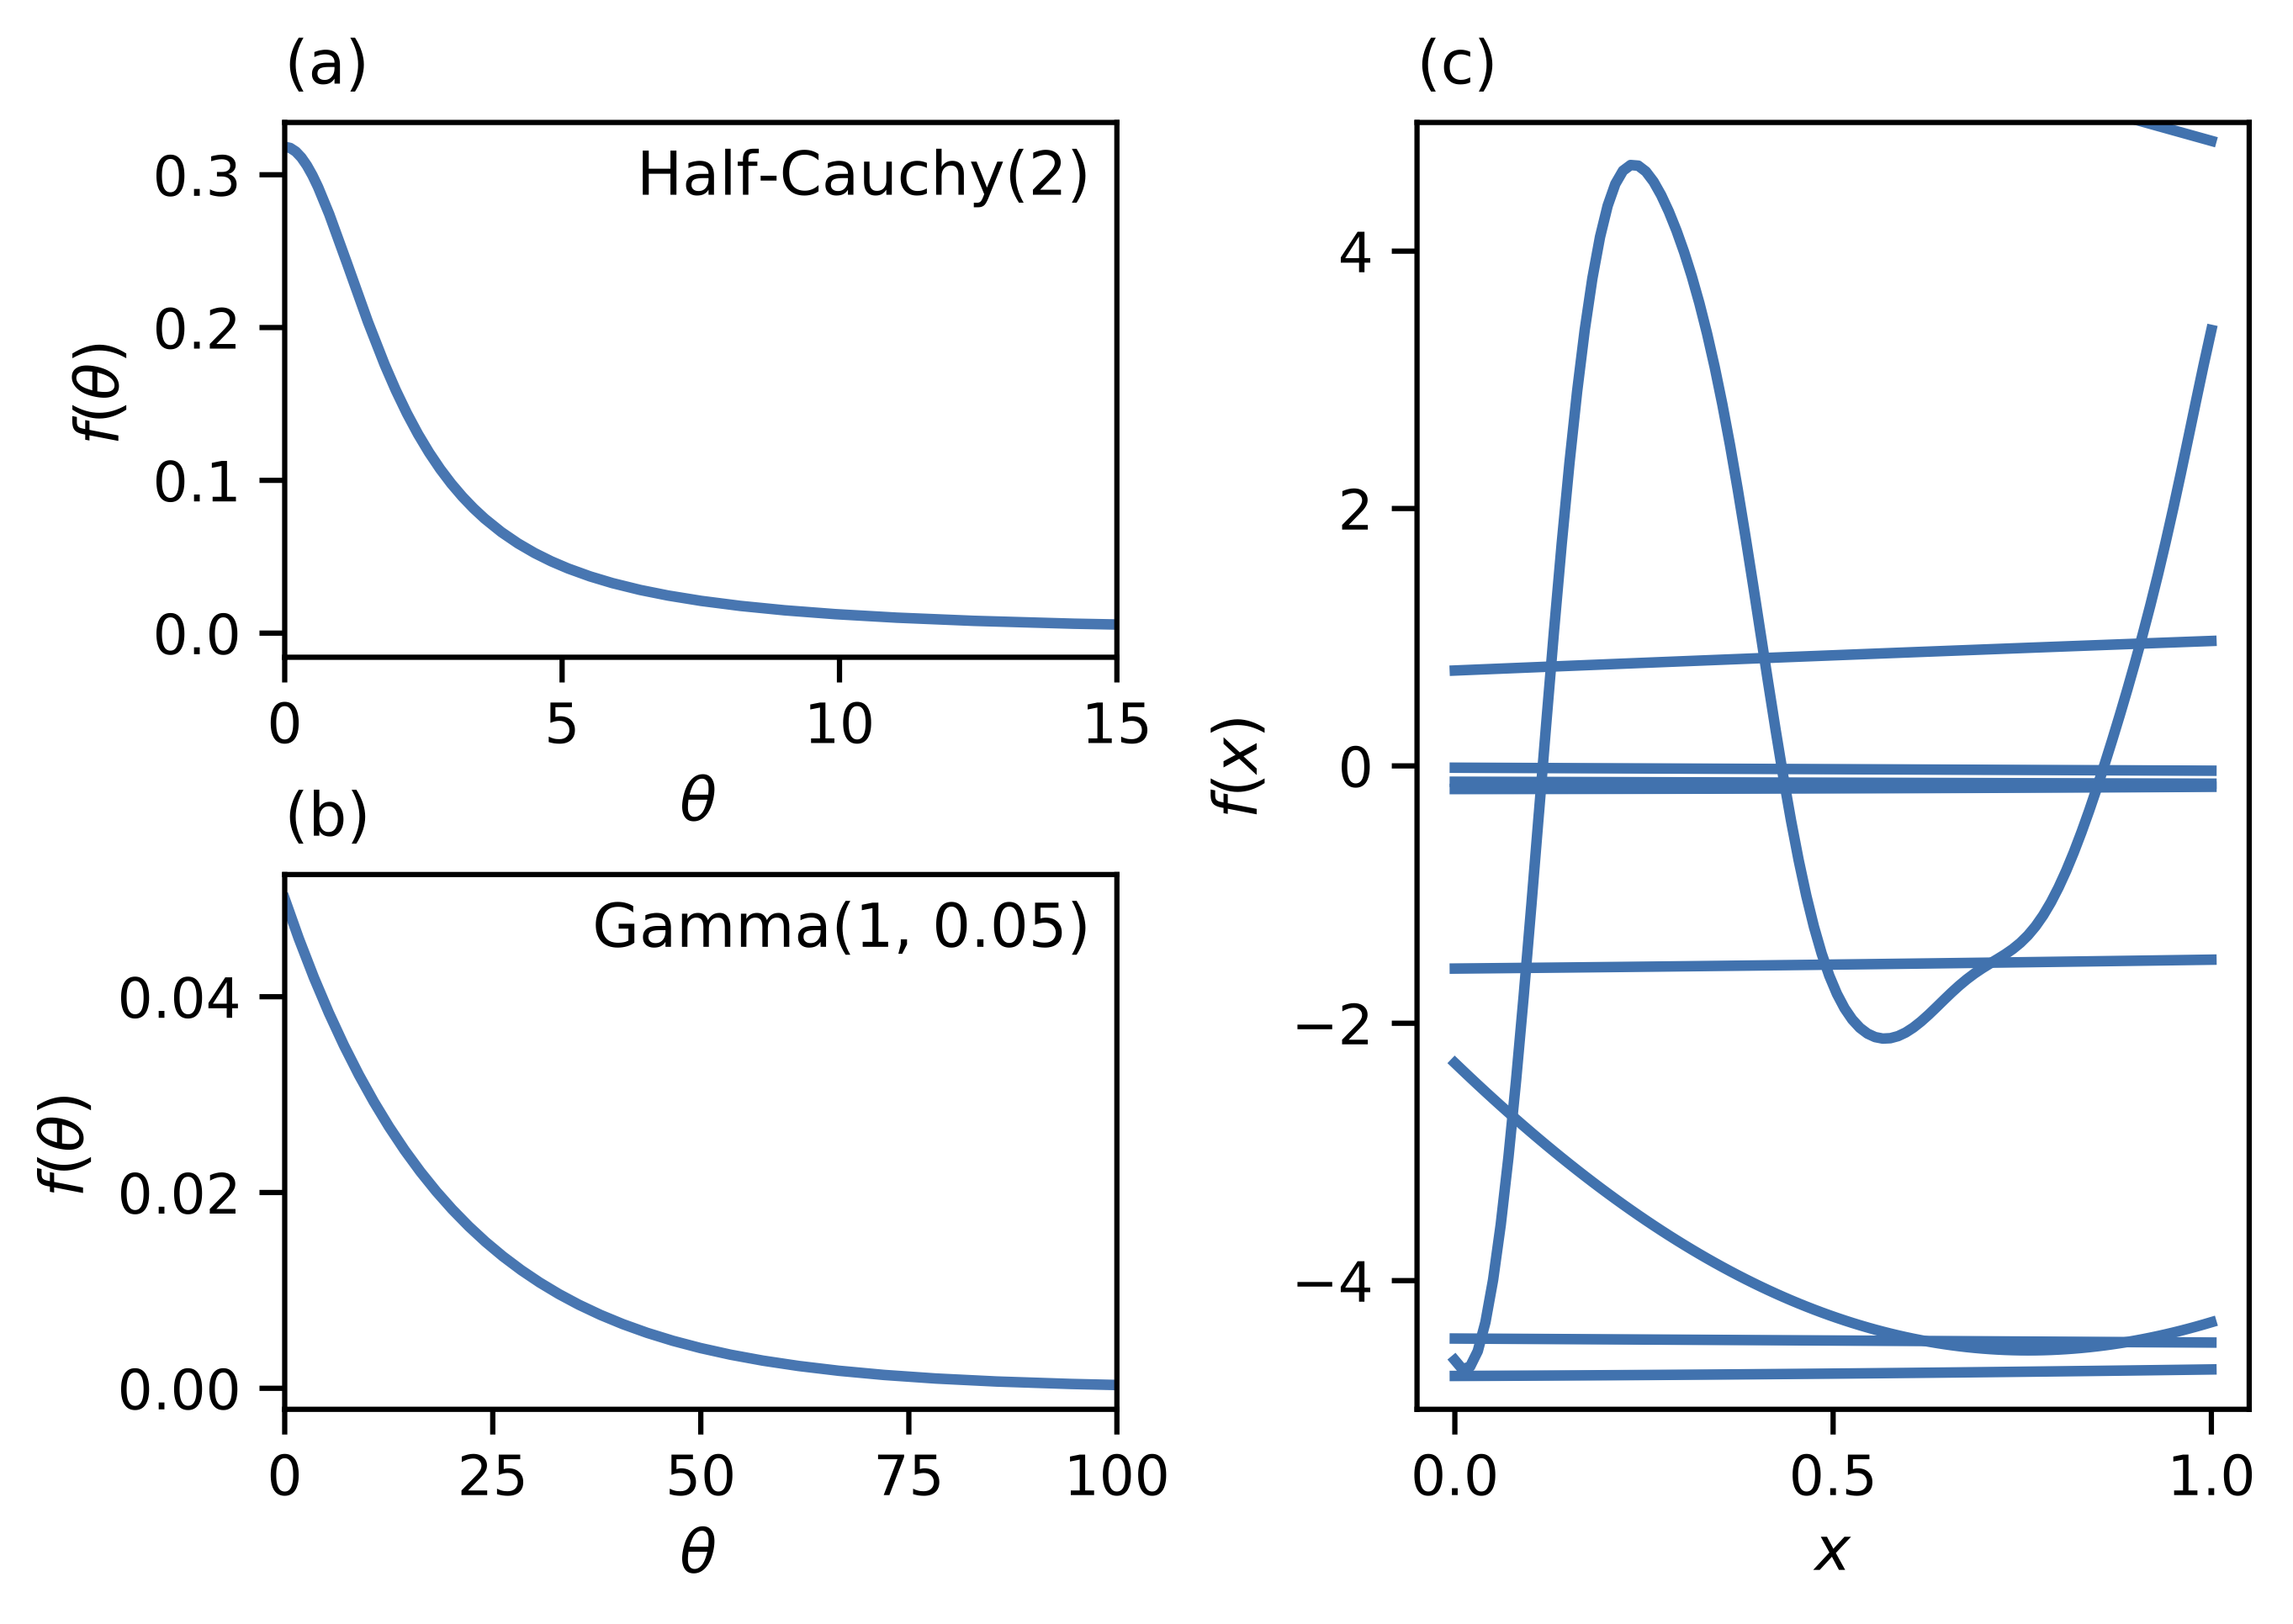
\includegraphics[width=0.8\textwidth]{chapters/msm_optimization/figures/prior_functions.png}
    \label{fig:priors}
\end{figure}

All predictors were scaled to lie in the range $[0, 1]$ to aid interpretation of the kernel length-scale parameters, $l$. Before scaling the integer predictors ($\tau$, $m$ and $n$) two other transformations, $T(\cdot)$, were considered: the identity $I(\cdot)$, and a logarithmic transformation, $\log(\cdot)$. The categorical predictor, $\chi$, was dummy coded \cite{dalyDummyCodingVs2016} to give a $d$ dimensional vector of $1$s and $0$s. For example the input vector, $\mathbf{x}$ for $n=10$ and $\chi=(\phi, \psi)$ is $\mathbf{x} = (1, 0, 0, 0, 0, 10)$, and for $n=10$ and $\chi=(x, y, z)$ is  $\mathbf{x} = (0, 1, 0, 0, 0, 10)$ and so on. 

In order to find the best GPR model for a given response surface, every combination of kernel function and integer predictor transformation was estimated and evaluated using the MAP estimates for the kernel hyper-parameters. This meant that for the response surface of alanine dipeptide with a single integer predictor, $8$ different models were estimated ($4$ different kernels and $2$ predictor transformations). For the response surface of AADH, with three integer predictors, $32$ different models were estimated ($4$ different kernels and $2\times2\times2=8$ different predictor transformations). 

In order to determine the best combination of kernel function and predictor transformation two model selection metrics were used:  mean standardised log loss (MSLL) and the standardised mean square error (SMSE). Each metric was calculated used 10-fold cross validation and any model with $MSLL > 0$ or $SMSE > 1$ was discarded. The remaining models were ranked separately according to MSLL and SMSE ($R_{MSLL}$, $R_{SMSE}$) and ranked according to $\sqrt{R_{MSLL}^2 + R_{SMSE}^2}$. This ranking method was used to ensure a balance between the two selection metrics. 

The final estimated response surface, $\hat{f}(\mathbf{\lambda})$, for alanine dipeptide and AADH was estimated using the full trial data set, $\mathcal{D}_{1:N}$. It is always possible to sample more hyper-parameters and add to the trial data set, which in principle would change $\hat{f}(\mathbf{\lambda})$ and so for completeness the estimate response surface should be written $\hat{f}(\mathbf{\lambda}; \mathcal{D}_{1:N})$. This dependence on $\mathcal{D}$ is due to the finite amount of hyper-parameter trials used to estimate the response surface, the true response surface $f(\mathbf{\lambda})$ has no dependence on the number of trials. 

All GPR modelling was performed with the Python package PyMC3 \cite{salvatierProbabilisticProgrammingPython2016} with some visualisation performed using package GPy \cite{gpy2014}. 

\subsection{Hyper-parameter relevance}\label{subsec:meth_rel}
The characteristic length-scales of the GP kernels, $l$, determine the correlation of the response between points with different values of the accompanying predictor. For $l=1$ with an exponential kernel then inputs separated by $|x-x^{\prime}|= 1$ will on average have a correlation of $\exp^{-0.1}\simeq 0.9$. This means for large values of $l$ the response with respect to changes in $x$ will be flat, or in other words, $x$ is irrelevant to determining the response. This prompts the definition of \emph{relevance}, $R = \sfrac{1}{l}$: when $R$ is large, the small changes in $x$ result in larger changes in the response, meaning it is relevant to determining the response. Henceforth, the kernel functions (equations \ref{eqn:kern_exp} - \ref{eqn:kern_m52}) will be parameterized by $R$ instead of $l$. 

The relevance of the MSM hyper-parameters is important quantity and so to calculate the uncertainty a fully Bayesian approach was used. The same GP model was used to calculate the relevance as was used in modelling the response surface, i.e. same kernel and same predictor transformations. Instead of using the MAP estimates for the GP hyper-parameters, the full posterior distribution was sampled using Markov Chain Monte Carlo and a No U-Turn sampler with two independent chains with $500$ tuning steps and $1000$ sampling steps. Convergence was checked using the R-hat statistic (\cite{gelmanBayesianDataAnalysis2014}). 


\subsubsection{MSM Optimization}\label{subsec:meth_opt}
The maximum of the response surface \emph{at the trial values} (known as the incumbent $(\mu^{*}, \mathbf{\lambda}^{*}$, \cite{shahriariTakingHumanOut}) gives the optimum hyper-parameters  by making full use of all the trial information. Bayesian optimisation was used to determine whether it is possible to arrive at the same incumbent, or better, using a smaller number of trials. A limited optimisation procedure was first performed on alanine dipeptide to demonstrate its effectiveness and to determine some of its parameters. A more extensive optimisation procedure was then performed on AADH. General introductions to Bayesian optimisation which cover all the methods used here can be found in \cite{snoekPracticalBayesianOptimization} and \cite{shahriariTakingHumanOut}. 

Bayesian optimization is a method for optimizing ``black-box'' objective functions - those which can be sampled from but are otherwise unknown. The response of an MSM to its hyper-parameters is a black-box objective function because it is not possible to determine the response without first fitting the MSM. Bayesian optimisation is a type of sequential model based \cite{hutterSequentialModelbasedOptimization2011} optimisation technique. These techniques entail first sampling the response of the objective function over its search space to create a trial data set. A statistical model called the \emph{surrogate function}, which serves as a proxy for the objective function, is built using the sampled responses. An utility function, known as the \emph{acquisition function}, determines the anticipated utility of a set of inputs in optimizing the objective function, based on the predictions and uncertainty in the surrogate function.  The objective function is then sampled using the set of inputs which maximize the acquisition function. This new trial is added to trial data set and process repeated. This algorithm in summarised in xxx. 

The surrogate function used was a GPR model with kernel and predictor transformations chosen using the method described in section \ref{sec:rsm} using the MAP estimates of the hyper-parameters of the GPR, $\theta$. The number of trials used to seed the surrogate function was determined by performing the optimisation seeded with $N=10, 30, 50$ trials, each repeated 10 times, and comparing the trajectory of the incumbent, its uncertainty and the consistency of the MSM hyper-parameters. The acquisition function used was the \emph{expected improvement} which gives the difference between the current incumbent and the  response at a given input, averaged using the uncertainty of the response. The improvement, $I$ at an input value $\mathbf{x}$ over the incumbent, $\mu^{*}$, using the response of surrogate function, $f(\mathbf{x}; \theta) = \nu_{N} \sim \mathcal{N}(\mu_{N}(\mathbf{x}), \sigma_N^{2}(\mathbf{x}))$, is defined as: 

\begin{equation}
    I(\mathbf{x}, \nu_{N}, \theta; \mu^{*}):=(\nu_{N} - \mu^{*}) \mathbb{I}(\nu_{N} > \mu^{*})
\end{equation}

Here the $\mathbb{I}$ is an indicator function which prevents the improvement from being negative and the subscript $N$ denotes the dependence of the distribution of $\nu$ on the data used to estimate $f(\mathbf{x})$. The expected improvement is the expectation of $I$, averaged over the distribution of $\nu$ which can be calculated analytically as: 

\begin{align}
        \alpha_{EI}(\mathbf{x}; \mathcal{D}_{N}) & := \mathbb{E}\left[I(\mathbf{x}, f(\cdot; \theta), \mu^{*})\right] \\
        & = (\mu_{N}(\mathbf{x}) - \mu^{*})\Phi\left( \frac{ \mu_{N}(\mathbf{x}) - \mu^{*} }{\sigma_{N}(\mathbf{x} } \right ) + \sigma_{N}(\mathbf{x})\phi\left( \frac{ \mu_{N}(\mathbf{x}) - \mu^{*} }{\sigma_{N}(\mathbf{x} } \right )
\end{align}

It is possible to take the expectation over both the distribution of $\nu$ and of the GP hyper-parameters $\theta$, this has been suggested and shown to be effective \cite{snoekPracticalBayesianOptimization}). However this was not done in this work because the extra computational cost involved. The candidate MSM hyper-parameters were determined as those which had the highest expected improvement as calculated on a $4 \times 100 \times 20 \times 100$ ($\chi \times \tau \times m \times n$) evenly spaced grid over the search space.

10 steps of this optimization procedure was performed on 10 random subsets of the alanine dipeptide trial data  set with $N=10, 30, 50$ observations  (stratified over the features $\chi$), corresponding to $5, 15, 25$ observations per predictor. These numbers were arbitrarily chosen but were influenced by conventional advice for parametric regression models (\cite{harrelRegressionModelingStrategies2015}) which states that the number of observations should be at least $15$ observations per predictor, thus $5, 15$ \& $25$, observations per predictor constituted a low, medium, and high information cases.  As discussed further in subsection \ref{subsec:ala1}, $25$ observations per predictor was found to result in satisfactory improvement in the incumbent and so was chosen as the number of trials used to seed the optimization procedure for AADH. 

It was observed during these experiments that the same candidate hyper-parameters were being proposed by the algorithm. This was deemed partly due to the simple nature of the response surface and partly due to the granularity of the grid used in the maximisation of the acquisition function. To ensure that each candidate hyper-parameter is unique, the Bayesian optimisation algorithm was modified so that only  hyper-parameters sets not already in the trial data set were considered as candidates. The final Bayesian optimisation algorithm is described in algorithm \ref{alg:bayes_opt}.

\begin{algorithm}\label{alg:bayes_opt}
\KwData{Trial data: $\mathcal{D}_{N} = \{(y_{1}, \mathbf{x}_{1}), ...,(y_{N}, \mathbf{x}_{N}) \}$}
\KwData{Search space grid: $\mathbf{X} = \{(\chi_1, \tau_1, m_1, n_1), ...,(\chi_{M}, \tau_{M}, m_{M}, n_{M})\}$}
\KwResult{$\mathbf{x}^{*} = \argmax_{\mathbf{x}}{f(\mathbf{x}; \mathcal{D}_{N+p})}$}
\BlankLine
\For{$i\leftarrow N$ \KwTo $N+p$}{
    estimate GPR $f(\mathbf{x}; \mathcal{D}_{i})$\;
    calculate incumbent: $\mu^{*} = \argmax{f(\mathbf{x};\mathcal{D}_{i})}\ \mathrm{s.t.}\ (y, \mathbf{x}) \in \mathcal{D}_{i}$\;
    estimate acquisition function: $\alpha_{\mathrm{EI}}(\mathbf{x}; \mathcal{D}_{i})\ \mathbf{x} \in \mathbf{X}$\;
    select candidate: $\mathbf{x}_{i+1} = \argmax_{\mathbf{x}}\alpha_{\mathrm{EI}}(\mathbf{x}; \mathcal{D}_{i})\ \mathrm{s.t.}\ (\mathbf{x} \in \mathbf{X})\ \&\ (\mathbf{x} \notin \mathcal{D}_{i})$\;
    query objective function to obtain: $y_{i+1}$\;
    augment data: $\mathcal{D}_{i+1} \leftarrow \{\mathcal{D}_{i}, (y_{i+1}, \mathbf{x}_{i+1})\}$
}
\caption{Bayesian Optimisation}
\end{algorithm}

For AADH two optimisation experiments were performed:
\begin{enumerate}
    \item $p=50$ steps of Bayesian optimisation was performed using a response surface seeded with all of the randomly sampled hyper-parameter trial data ($N=361$);
    \item $p=50$ steps of Bayesian optimisation was performed on five subsets  of the hyper-parameter trial data with  $N=100$.
\end{enumerate} 
In both cases the kernel and input transformations were determined using the method in section \ref{sec:rsm}. 


\section{Results and discussion}
\subsection{Alanine Dipeptide}\label{subsec:ala1}
\subsubsection{Response surface}\label{subsubsec:ala_rsm}
The average MSM response for each trial are shown in figure \ref{fig:ala1_train_test}. The test response ($f^{test} = f(\chi, n; x^{test})$, blue points) and the degree of over-fitting ($f^{train} - f^{test}$, orange) are shown as a function of $n$. The  features are ordered according to the  mean of the test response. As expected the  $(\phi, \psi)$ feature has the highest average response. Perhaps unexpectedly, the heavy atom $(x,y,z)$ coordinates feature performs almost as well. Each feature shows an almost flat response to increasing $n$ and each with a negligible degree of over-fitting. 
The test response was modelled as a Gaussian Process with $\chi$ and $n$ as predictors. Model selection on the combinations of kernel functions and predictor transformations was performed and the results are shown in table \ref{tab:ala2_fit_results}.  

The largest improvement in fit, as measured by both the MSLL and SMSE, comes from changing the transformation from $I(n)$ to $\log{(n)}$. This is unsurprising given that the shape of the response for the $(\phi, \psi)$ and $(x,y,z)$ features (panels (a) and (c) in figure \ref{fig:ala1_train_test}) is a clearly non-stationary process: the correlation with respect to changes in $n$ is much lower for $n\leq 100$ than for $n\geq 100$ where the response is flat. The log transformation smooths the response with respect to $n$ and makes the assumption of a stationarity more plausible. The best fitting model, as judged by both the smallest SMSE and MSLL, uses a log transformation of the number of clusters and $k_{M}$ in \ref{eqn:kernel_form} equal to a Mat{\'e}rn 5-2 kernel \ref{eqn:kern_m52}. I use these two modelling choices in all further modelling of the alanine dipeptide response surface.  

The response surface for alanine dipeptide is shown in figure \ref{fig:ala1_response}.  The blue line shows the mean of the Gaussian process and the shaded blue area represents two standard deviations about the mean value (i.e. the width of the Gaussian process but ignoring the predicted measurement error, $\sigma_n$). This response surface fits the observed data well, both in terms of the mean response and its uncertainty. There are a number of features of the response surface which are worth discussing. 

\begin{figure}[ht]
    \centering
    \caption{The response surface for MSMs of alanine dipeptide as a function of the feature, $\chi$ (panels a - e) and number of clusters, $n$ (horizontal axis).  }
    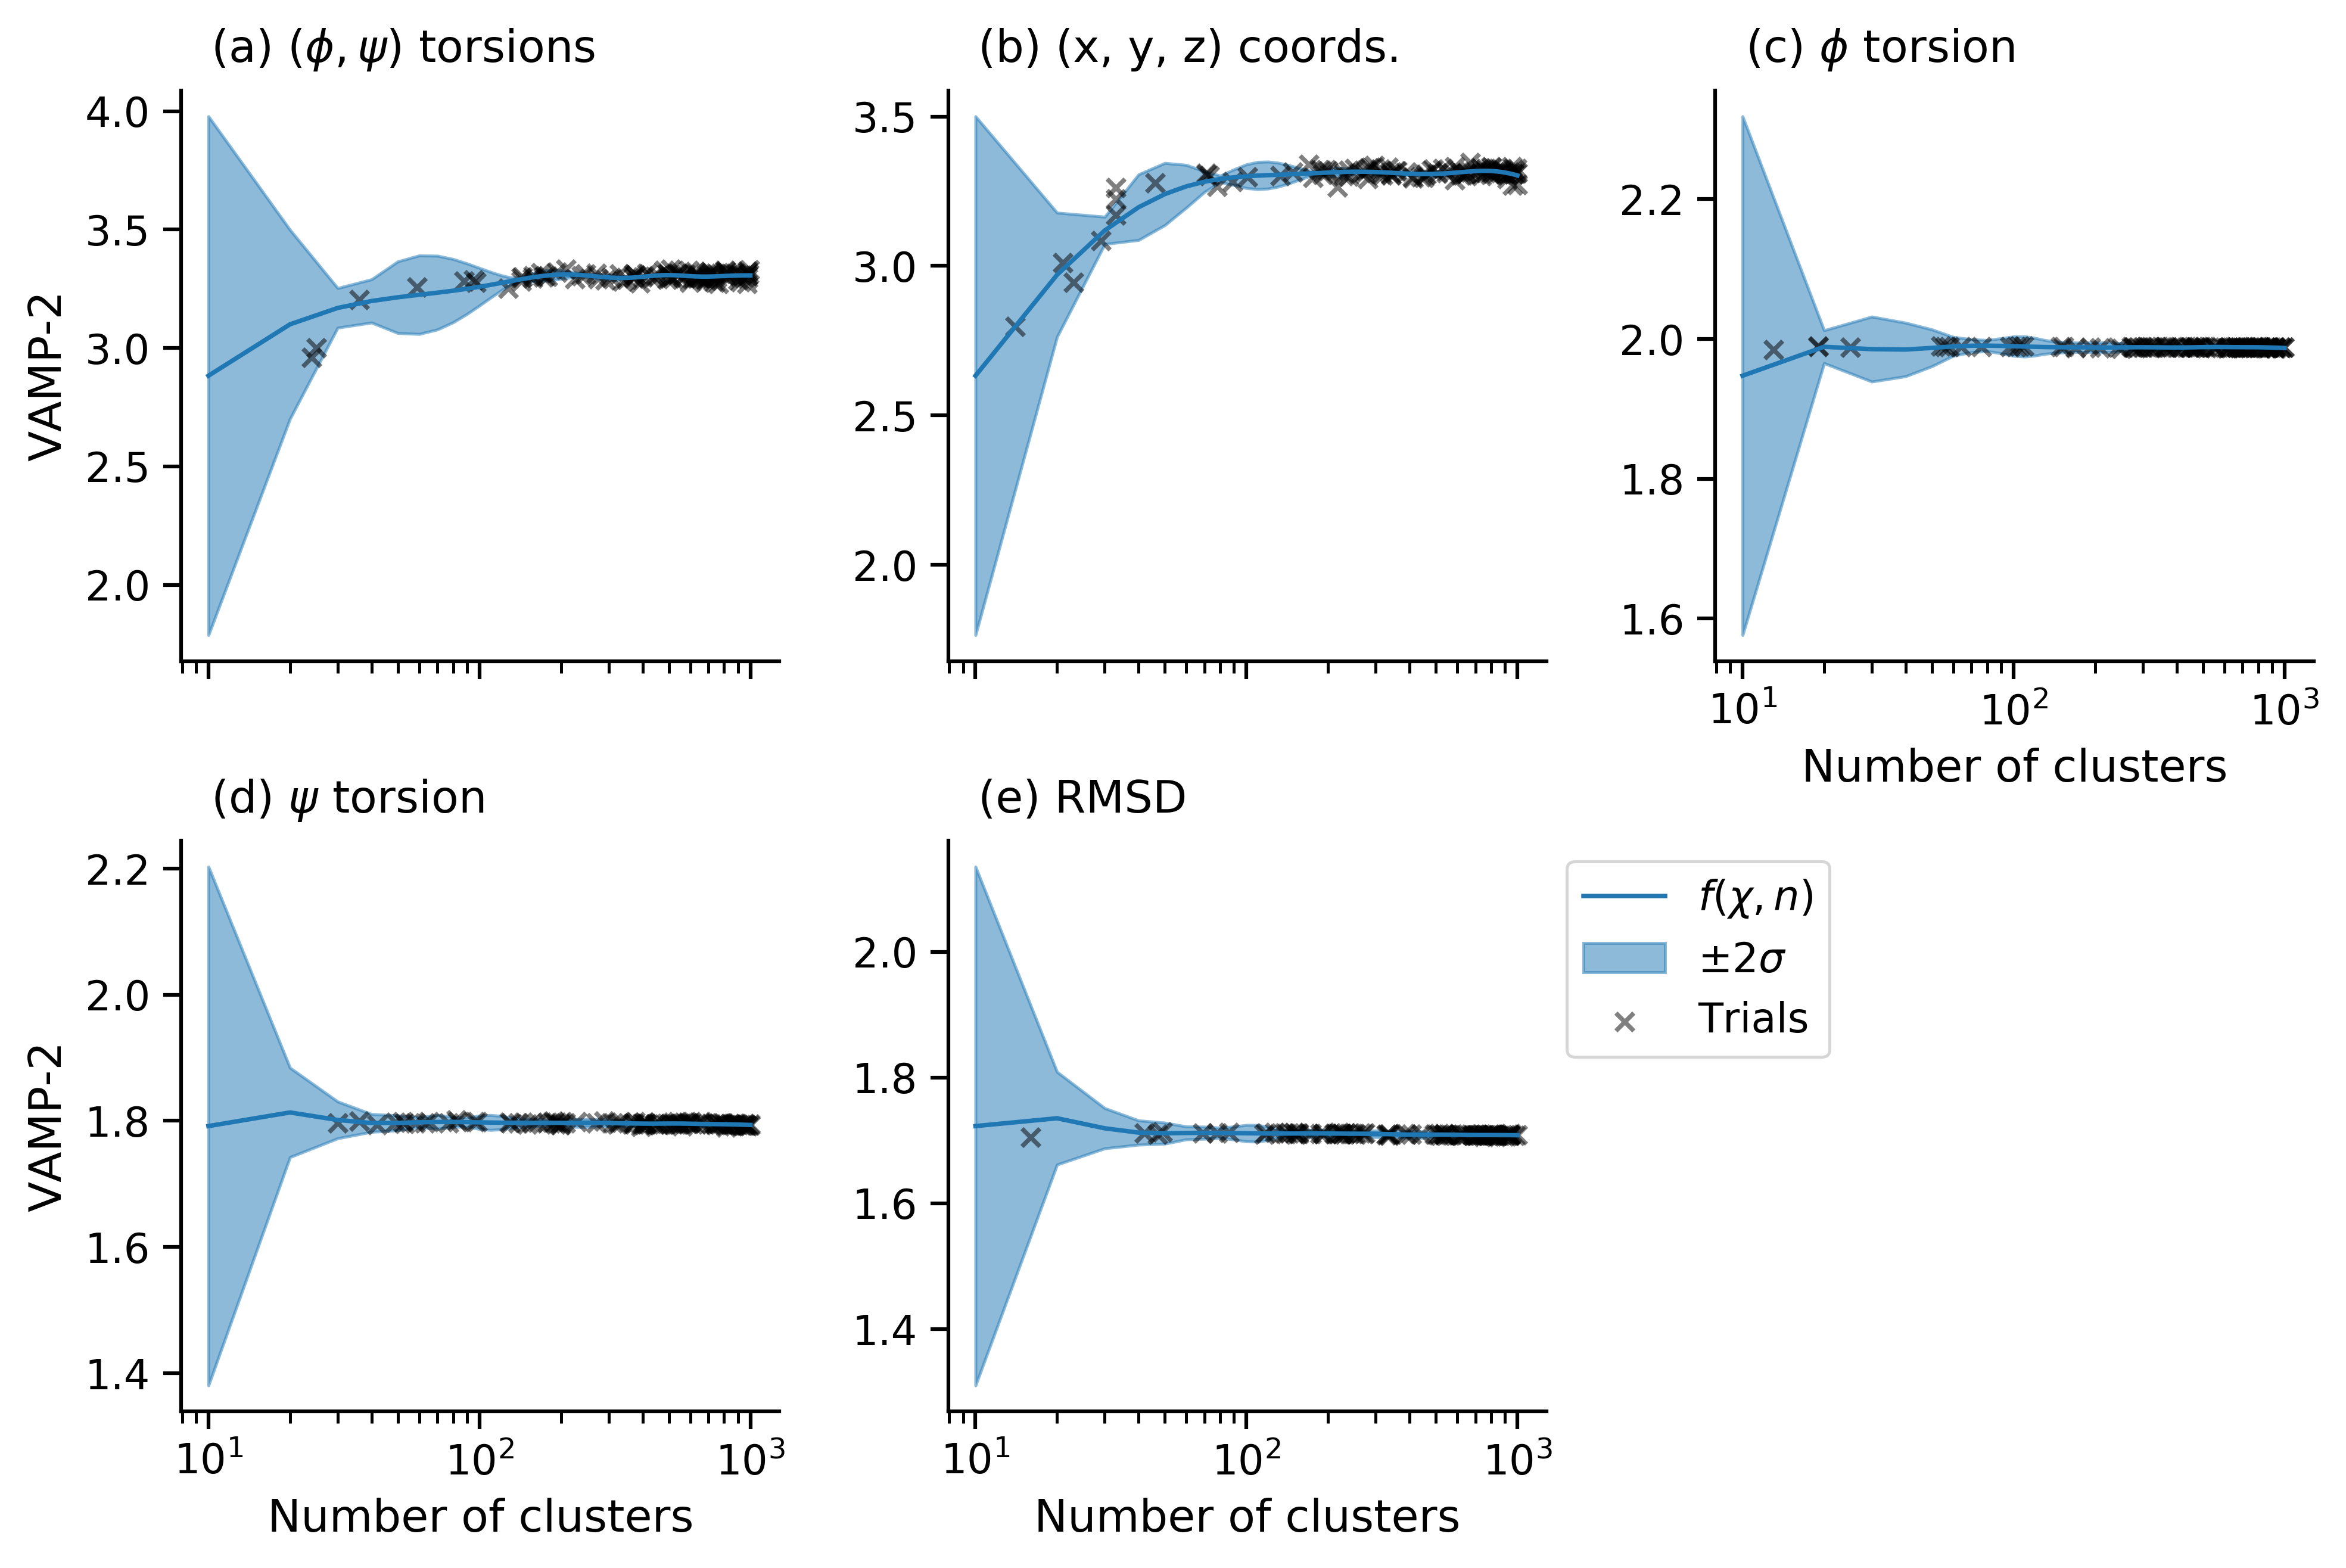
\includegraphics[width=0.8\textwidth]{chapters/msm_optimization/figures/ala1_response_surface.png}
    \label{fig:ala1_response}
\end{figure}

First, for there is a decrease in response as $n \rightarrow 10$ for the $(\phi, \psi)$ and $(x,y,z)$ coordinate features but not the remaining features (although this is due to the sparse sampling for $n<20$ and no sampling for $n<10$). This is expected from from previous studies \cite{wuVariationalApproachLearning2019}\cite{mcgibbonVariationalCrossvalidationSlow2015} and is due to decreasing eigenfunction discretization error, $\delta$  \cite{prinzMarkovModelsMolecular2011} as a $n$ increases. In the language of statistical learning theory \cite{friedman2001elements}, this is the high ``Bias'' regime of the ``Bias-variance'' trade-off. The discretizaton error for the $i$'th normalized eigenfunction $\Psi_{i}$ is given by: 

\begin{equation}
    \delta_{i} \equiv\left\|\Psi_{i}(\mathbf{z})-\hat{\Psi}_{i}(\mathbf{z})\right\|_{\pi, 2}=\left(\int_{\Omega} d \mathbf{z} \pi(\mathbf{z})(\Psi_{i}(\mathbf{z})-\hat{\Psi}_{i}(\mathbf{z}))^{2}\right)^{1 / 2}
\end{equation}

Here $\mathbf{z}$ are the relevant coordinates of the system, $\pi$ is the stationary distribution and the integral runs over all of the state space, $\Omega$. Figure \ref{fig:ala1_evcompare} demonstrates this for the $\phi$ feature. Panel (a) shows the stationary distribution, which has been truncated for $\phi \simeq 0, 2$ due to the temporal resolution of the MD trajectories. Panels (b), (c) and (d) show the difference between the second normalised eigenvector ($\Psi_{2}$) estimated with $n=500$ basis states, (black line, labelled `True', because it assumes the discretization error here is negligible), and the same eigenvector estimated with $2, 5, 50$ basis states (blue line, labelled `Approx.'). The red shaded area shows the discretization error which decreases as $n$ increases as the approximate eigenfunction gets closer to the `True' eigenfunction. For this feature, and likely for the other 1D features, the largest increase in VAMP-2 occurs below $n=10$ which explains the the drop in response with decreasing $n$ is not observed. 

\begin{figure}
    \centering
    \caption{}
    \label{fig:ala1_evcompare}
    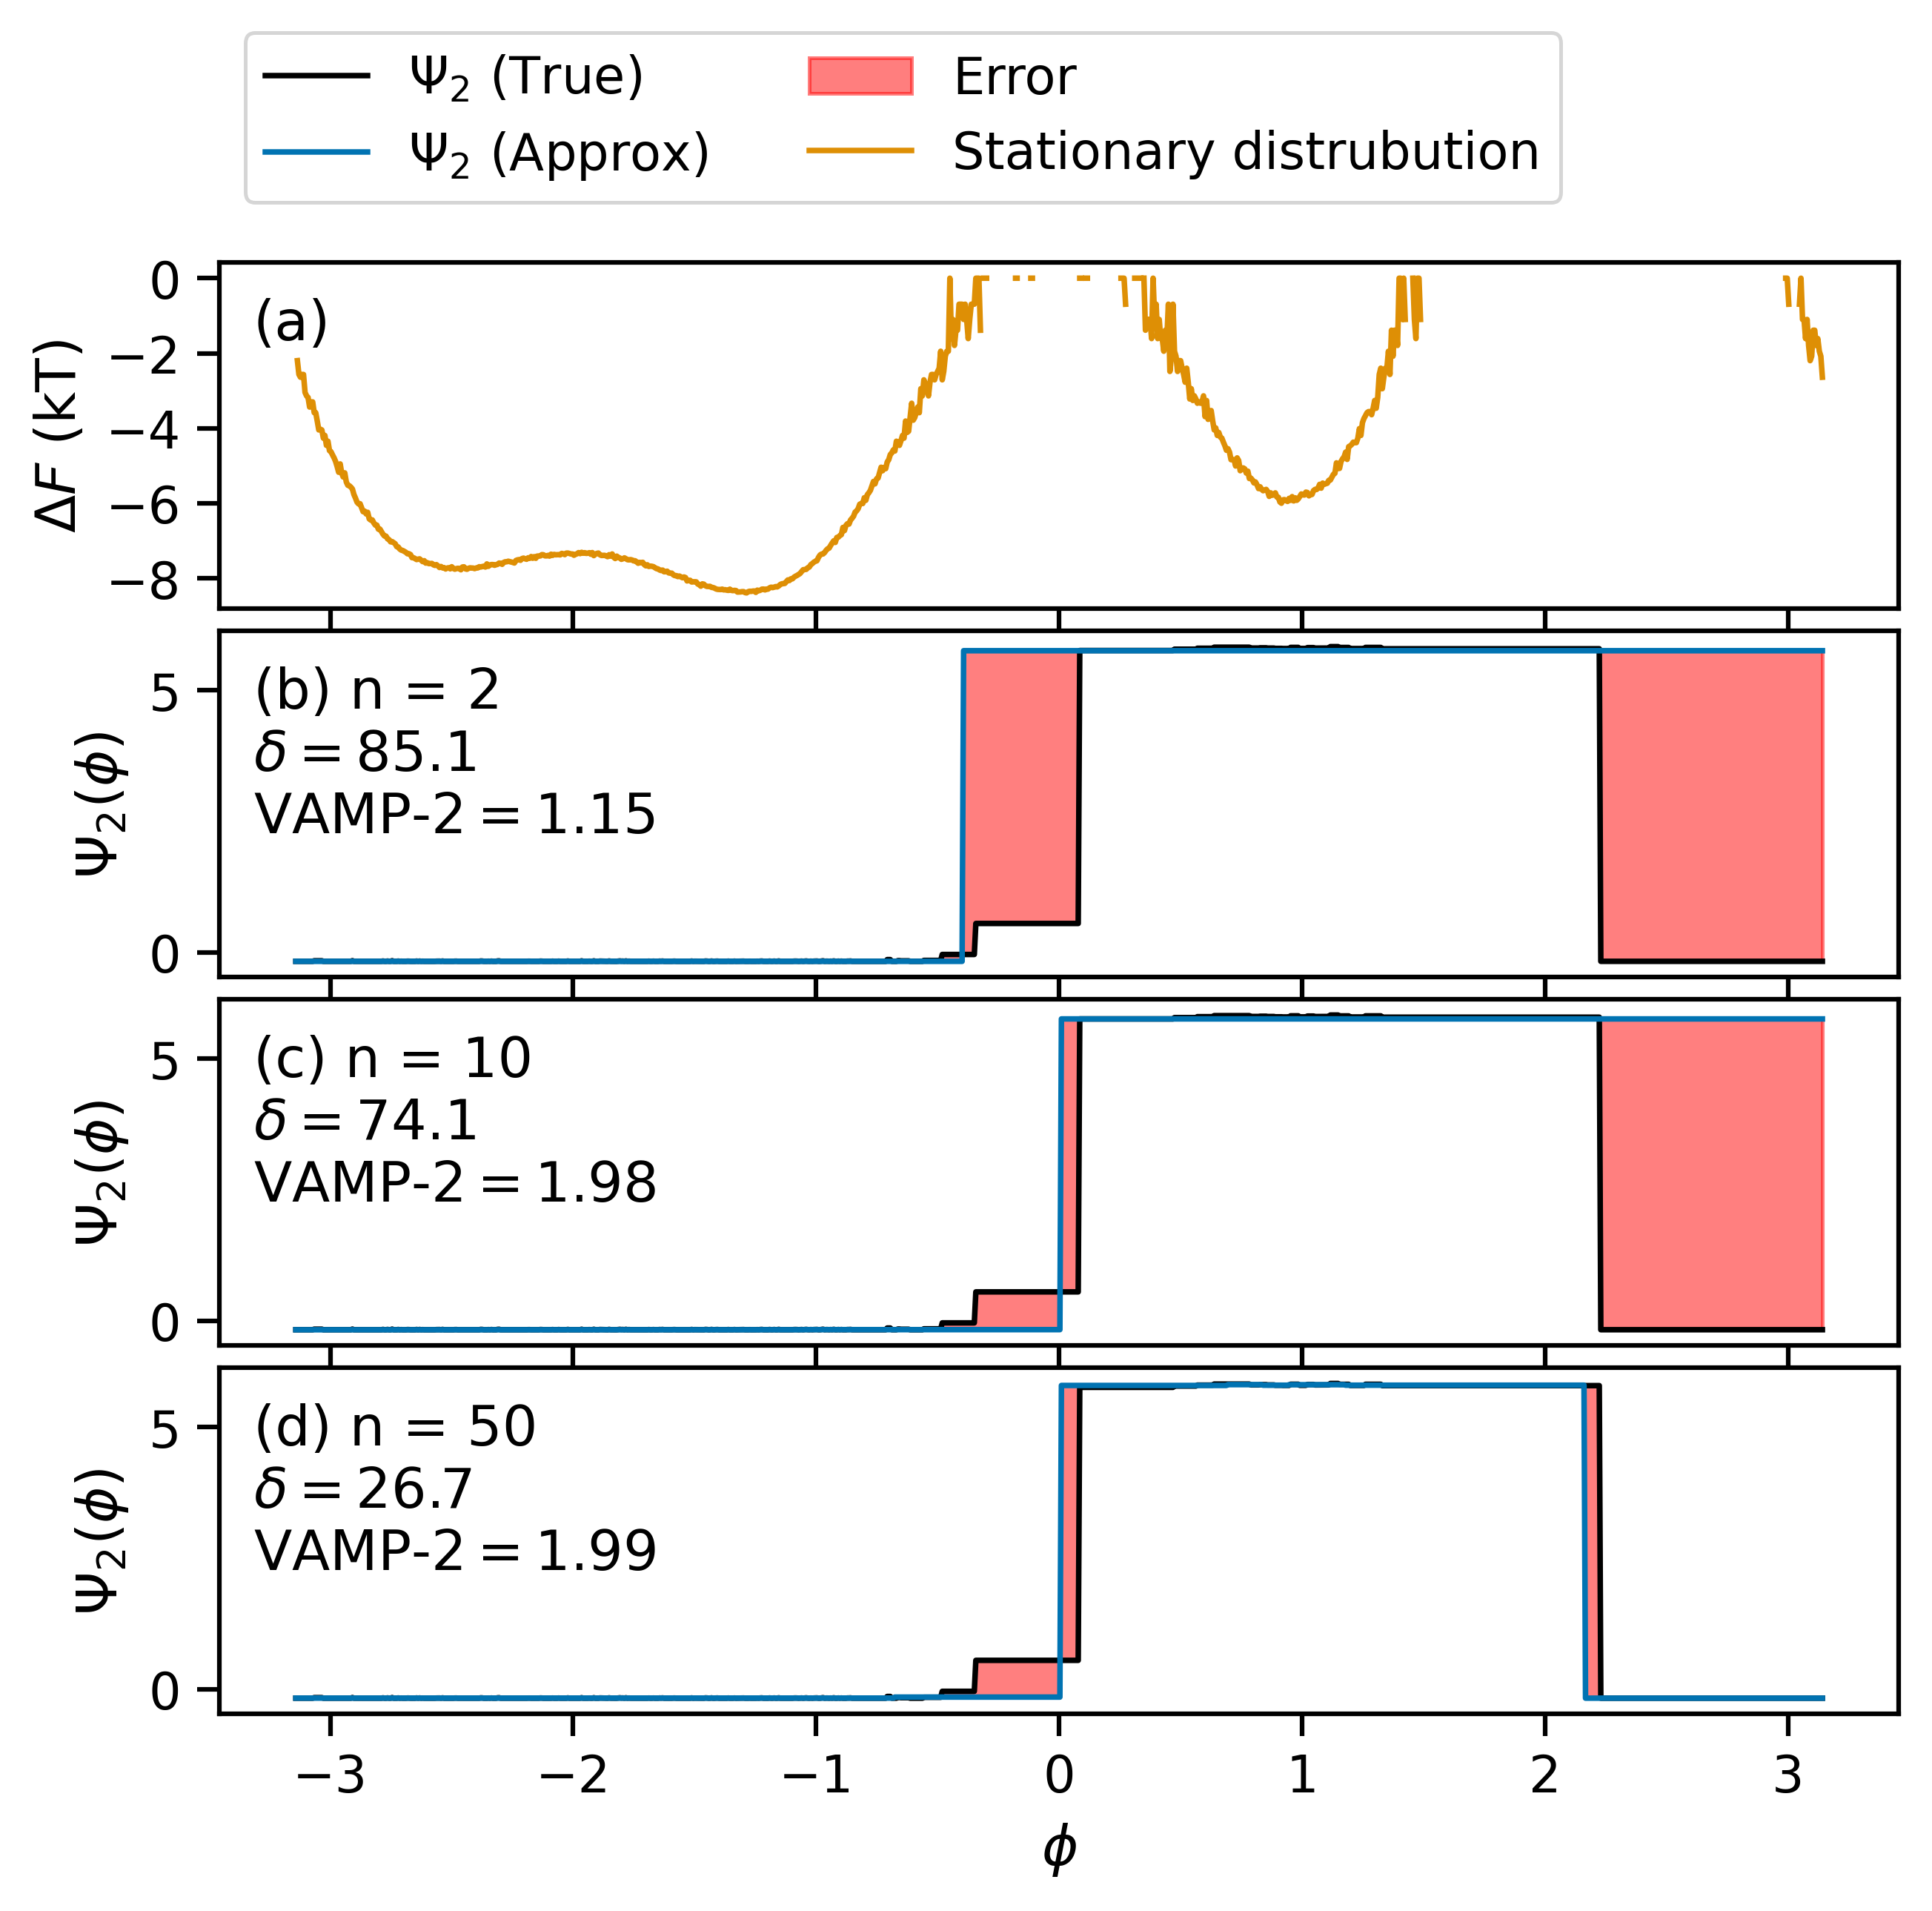
\includegraphics[width=0.8\textwidth]{chapters/msm_optimization/figures/ala1_ev_n_compare.png}
\end{figure}

Second, the response for $n > 100$ for all features is constant which is a result of the number of eigenvectors/eigenvalues used in the VAMP-2 score and the volume of MD data. Only the first $4$ non-trivial eigenvectors are used in the VAMP-2 score so the decrease in discretization error with increasing $n$ will eventually approach zero for these eigenvectors. As $n$ continues to increase we expect to enter the high variance regime of the ``Bias-variance'' trade-off as the number of transitions between states becomes smaller resulting in higher statistical uncertainty in the elements of transition matrix. 

Third, large uncertainty of response surface for $n \leq 20$ is a result of transformation of the $n$ into log-space and the comparatively sparse sampling in this region. Identifying the type of input transformation (or input \emph{warping})is important for efficient optimisation \cite{snoekInputWarpingBayesian2014} discussed further below in this chapter.

Fourth, it is clear from inspection of figure \ref{fig:ala1_response} that the most relevant hyperparameter for determining the test response is the feature, $\chi$, while the number of cluster centres,  $n$, is almost irrelevant. This information can be encoded the learned parameters of a Gaussian process regression model which will be of benefit in more complicated systems with more than two hyperparameters. 
 
\subsubsection{Hyper-parameter relevance}\label{subsubsec:ala_relevance}
This last observation can be quantified and understood by calculating the relevance of each predictor using the estimated length-scale parameters of the kernel. There are five levels of the categorical predictor $\chi$ each with an associated relevance ($R_{\chi_{1}}, ..., R_{\chi_{1}}$) as well as the relevance of the number of cluster centres, $R_{n}$. The interpretation of these two sets is slightly different. 

\begin{figure}
    \centering
    \caption{Box plots of the relevance of hyper-parameters of alanine dipeptide. The distribution of the parameters of the response surface (shown in figure \ref{fig:ala1_response}) were estimated using MCMC. The relevance of the features (levels of $\chi$) are shown in blue, labelled `Feature'. The relevance of the log-transformed number of cluster centres, $n$ is shown in orange (labelled `Other').}
    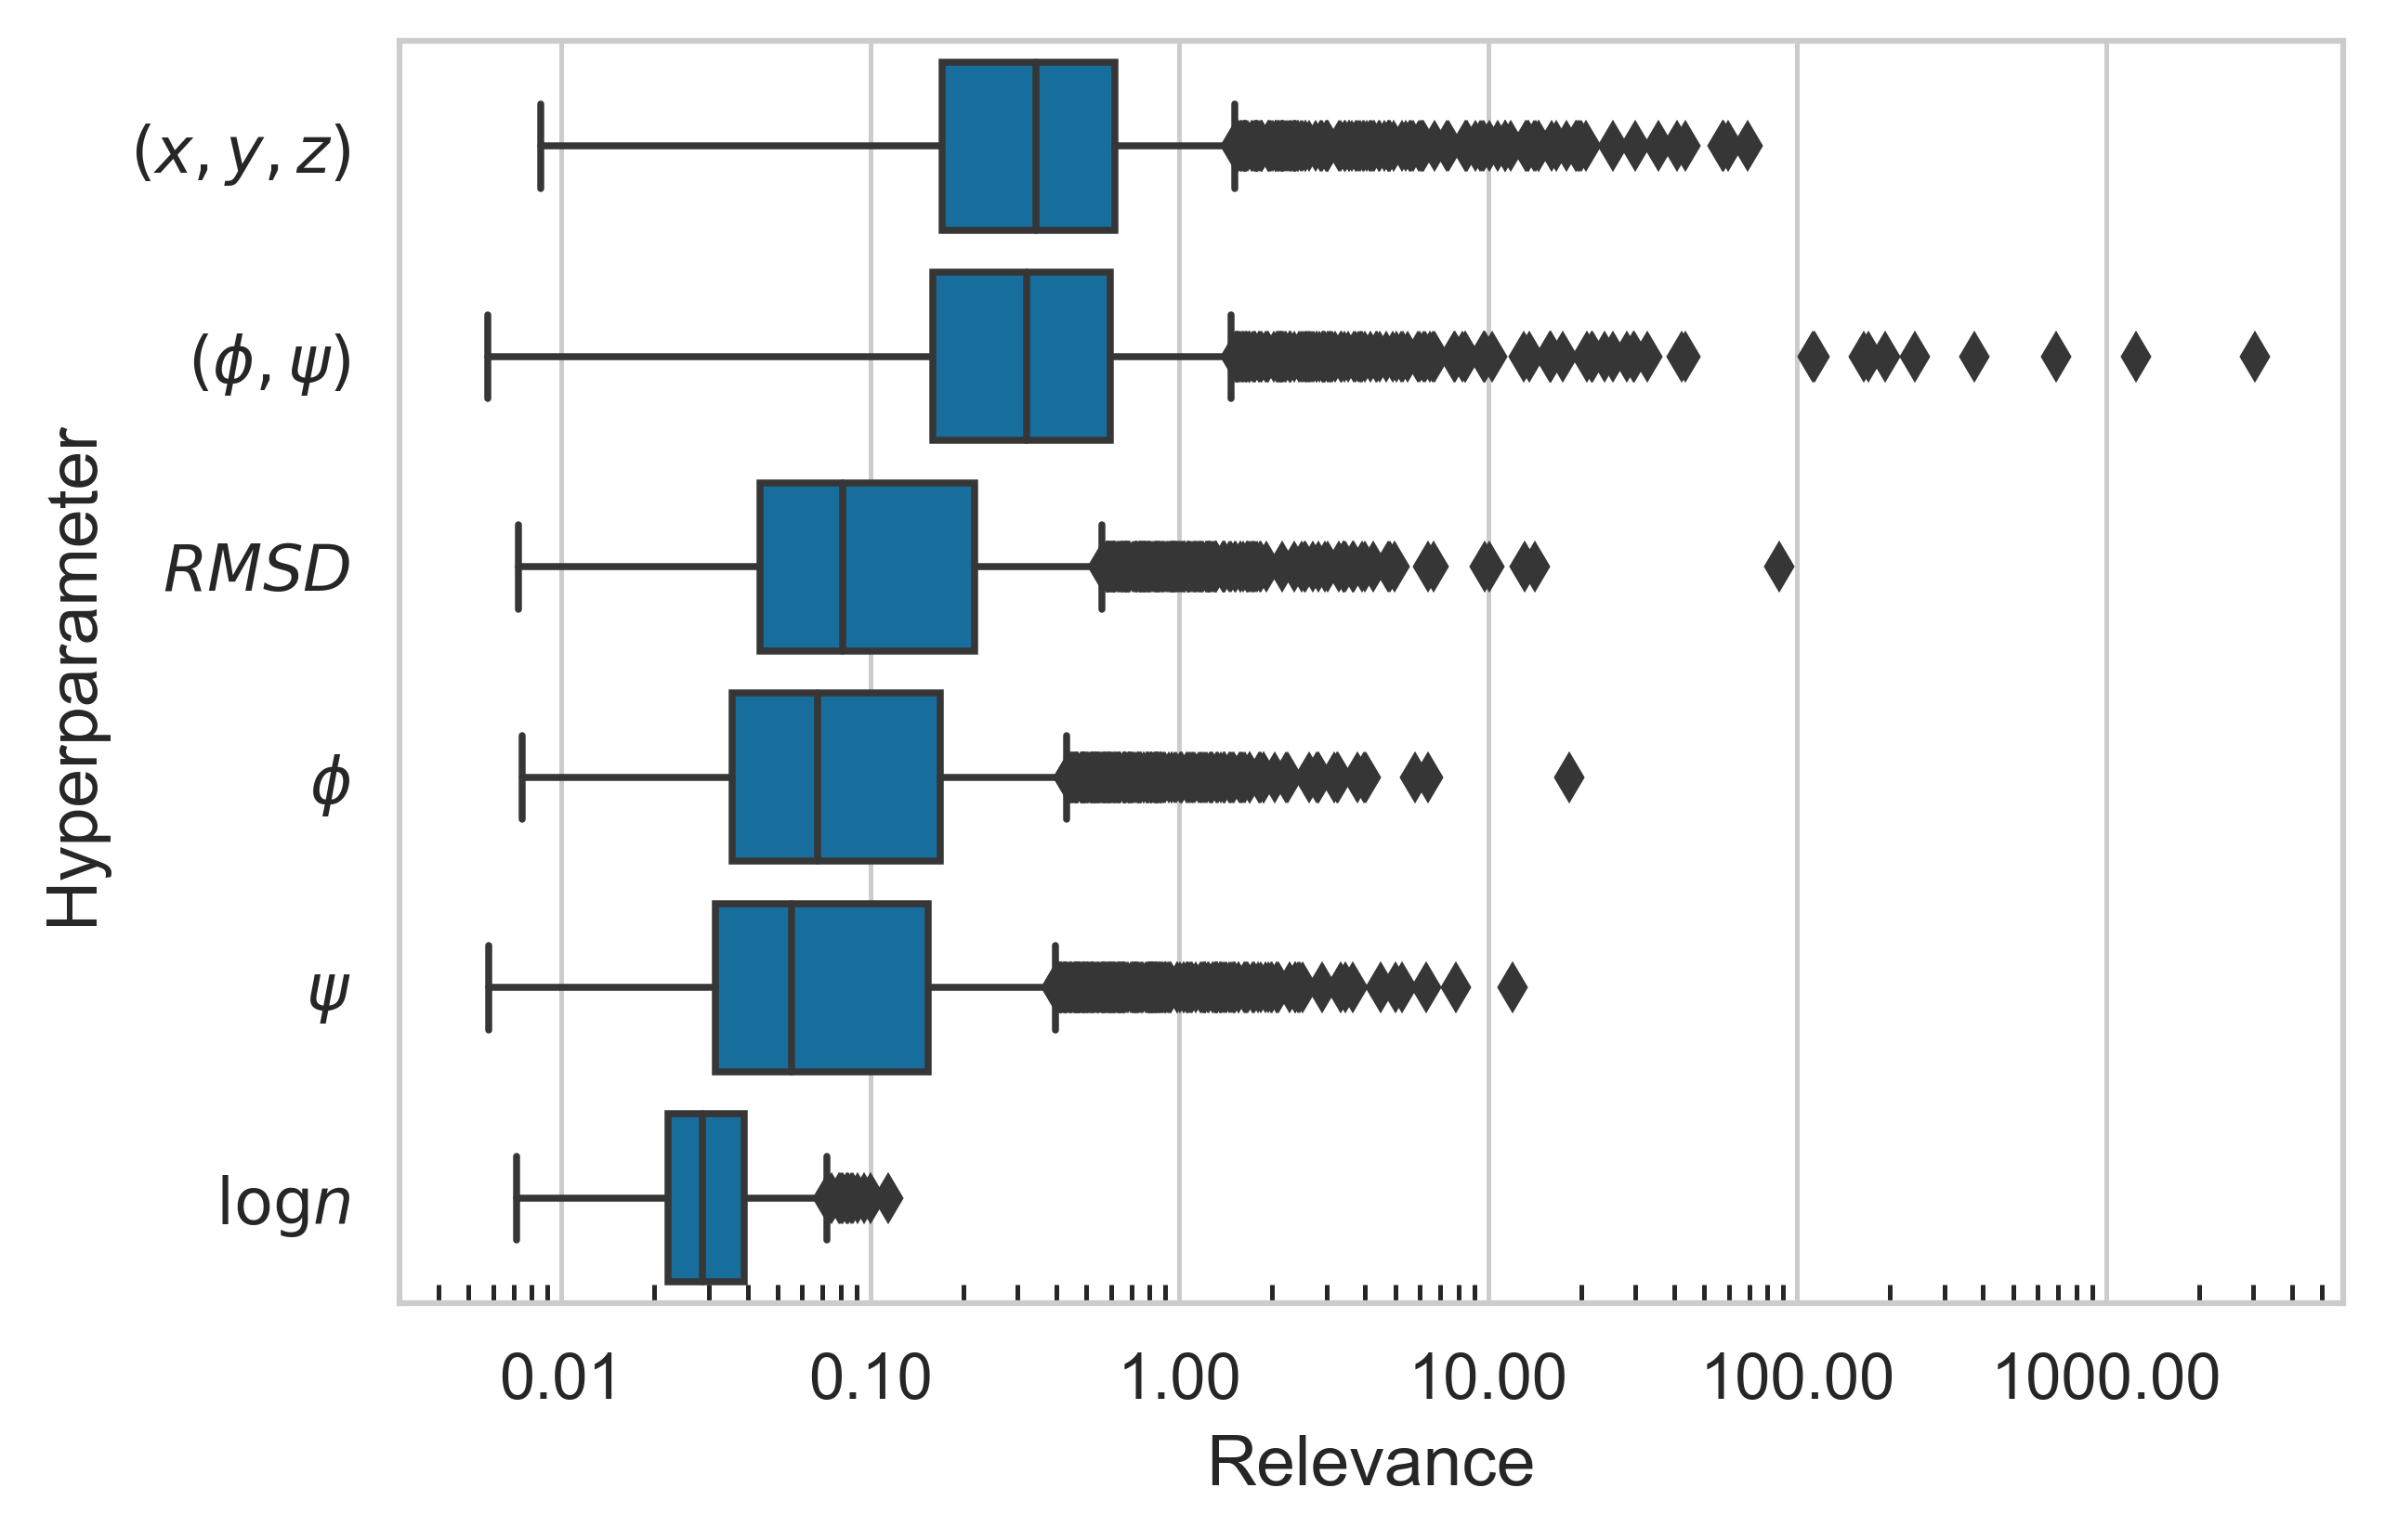
\includegraphics[width=0.8\textwidth]{chapters/msm_optimization/figures/ala1_relevance.png}
    \label{fig:ala1_relevance}
\end{figure}

\begin{table}
    \centering
    \caption{Caption}
    \begin{tabular}{|l|l|}
    \hline
                          Hyper-parameter &    Median (95\% C.I.) \\
    \hline\hline
     $R_{(\phi, \psi)\ \mathrm{torsion}}$ &  0.321 (0.020-4.456) \\
        $R_{(x, y, z)\ \mathrm{coords.}}$ &  0.344 (0.024-5.572) \\
             $R_{\phi\ \mathrm{torsion}}$ &  0.068 (0.015-1.176) \\
             $R_{\psi\ \mathrm{torsion}}$ &  0.056 (0.013-1.327) \\
                               $R_{RMSD}$ &  0.081 (0.016-1.406) \\
                          $R_{\log{(n)}}$ &  0.029 (0.013-0.063) \\
                                   $\eta$ &  2.518 (1.141-5.530) \\
                               $\sigma_n$ &  0.006 (0.006-0.007) \\
    \hline
    \end{tabular}
    \label{tab:ala1_rel_post}
\end{table}

The relevance of $n$ determines the correlation of the response to changes in $n$ \emph{within the same feature}. The covariance between $n$ and $n^{\prime}$ on the same feature will be (using the equation \ref{eqn:kernel_form})):

\begin{equation}
\begin{split}
    k^{tot}(\mathbf{x}, \mathbf{x}^{\prime})& = k\left((1, 0, 0, 0, 0, n), (1, 0, 0, 0, 0, n^{\prime})\right) \\
    & = \eta^{2}\cdot 1 \cdot 1\cdot 1 \cdot 1\cdot 1 \cdot k_{M}(n, n^{\prime}; R_{n}) \\
    & = \eta^{2}\cdot k(n, n^{\prime})
\end{split}
\end{equation}
In the last line the noise term $\sigma_{n}$, $\nu$ and $R$ have been dropped for clarity and use has been made of the fact that for kernels  $k(0, 0)=k(1,1)=1$. The covariance between the response at $n$ and $n^{\prime}$ is determined by the kernel parameter $R_{n}$ (and $\eta$ although this is the same for all predictors). The median values of the response surface parameters are shown in table \ref{tab:ala1_rel_post} and these imply that for change $n=10$ and $n=1000$ (a change of $1$ on the normalized scale) the correlation will be $k_{M52}(0,1; 0.029) \simeq 0.99$. 

The relevance of the different features determines the amount of information sharing between different features. Between a high relevance feature and all other features, there is little information sharing; between low relevance features there is a large amount of information sharing. To see this, consider the covariance between points at $n$ and $n^{\prime}$ on two different features, $\chi_1$ and $\chi_2$: 

\begin{equation}
\begin{split}
    k(\mathbf{x}, \mathbf{x}^{\prime})& = k\left((1, 0, 0, 0, 0, n), (0, 1, 0, 0, 0, n')\right) \\
    & = \eta^{2}\times k_{M}\left(1, 0; l_{\chi_1}\right) \times k_{M}\left(0, 1; l_{\chi_2}\right) \cdot 1 \cdot 1\cdot 1 \cdot k_{M}(n, n^{\prime}; l_{n}) \\
    &=  \eta^{2}\cdot k_{1}\cdot k_{2}\cdot k(n, n^{\prime})
\end{split}
\end{equation}

Here the notation is again simplified by making use of the fact that the kernel functions over different features can only take on value of $k_{i}(0, 1)=k_{i}(1, 0) = k_{i}(1)=k_{i}$. For low relevance features, low $R$ implies $k\simeq 1$ and the covariance of the response between $n$ on $\chi_1$ and $n^{\prime}$ on $\chi_2$ will be the similar to the covariance between $n$ and $n^{\prime}$ on the same feature. With high relevance features, high $R$ implies $k \ll 1$ and there will be little correlation between the response at $n$ on feature $\chi_1$ and $n^{\prime}$ on features $\chi_2$.   The features for alanine dipeptide are all relatively low relevance (i.e. less than $1$) which is a reflection of the  consistently flat response to changes in $n$ discussed above. However the $(\phi, \psi)$ and $(x,y,z)$ coordinate features have slightly higher relevance which is required to accommodate the drop in the response for low $n$ compared to the flat response for the other features.  

\subsubsection{Optimization}\label{subsubsec:ala_opt}

\begin{figure}[ht!]
    \centering
    \mycaption{Bayesian optimisation trajectories of alanine dipeptide seeded with 30 hyper-parameter trials, panel \ref{fig:ala_opt_traj_30},  and 50 hyper-parameter trials, panel \ref{fig:ala_opt_traj_50}, for five different random subsets  (`iterations') of the total hyper-parameter trial data set. The orange values are the trajectories calculated from random sampling, the blue values are the Bayesian optimisation trajectories. The first row (sub-panels (a) - (e)) are the VAMP-2 response, the second row (sub-panels (f) - (j)) show the accompanying number of cluster centres, and the third row (sub-panels (k) - (o)) are the  accompanying feature.}\label{fig:ala_opt_traj}
    \subtop[30 hyper-parameter trials\label{fig:ala_opt_traj_30}]{
        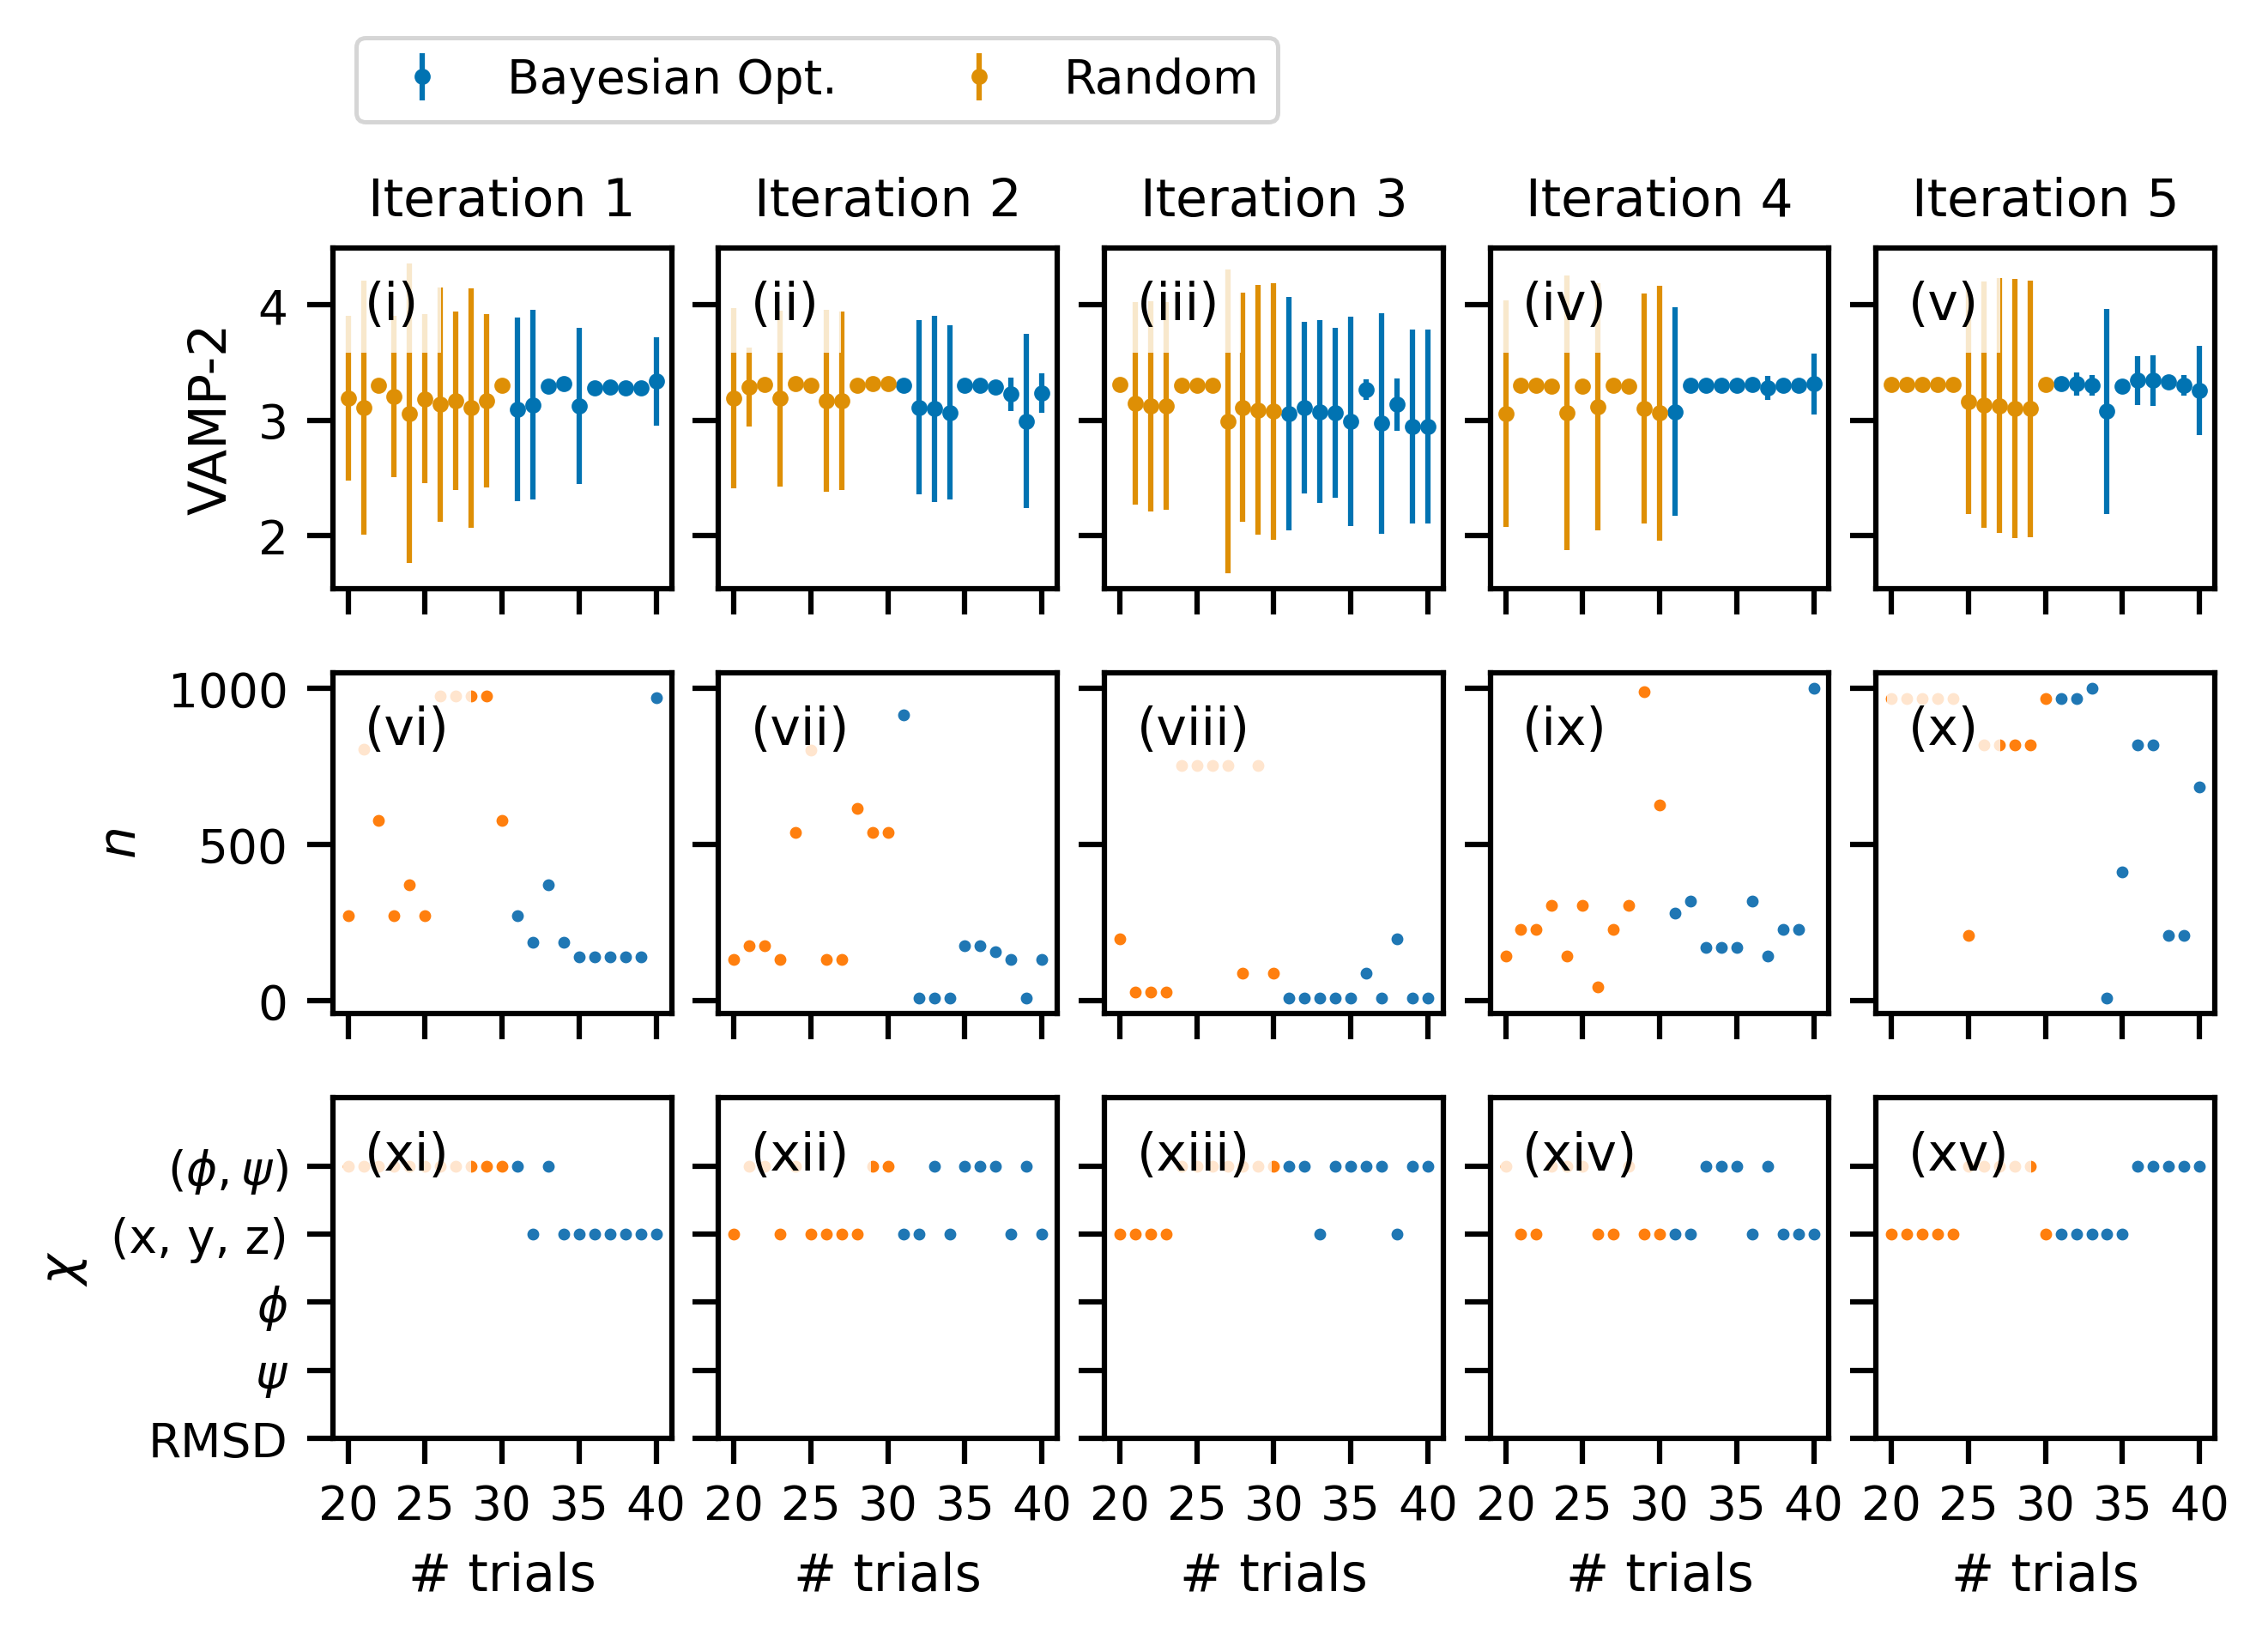
\includegraphics[width=0.8\linewidth]{chapters/msm_optimization/figures/ala1_opt_traj_start_obs_30.png}}
    
    \subtop[50 hyper-parameter trials\label{fig:ala_opt_traj_50}]{
        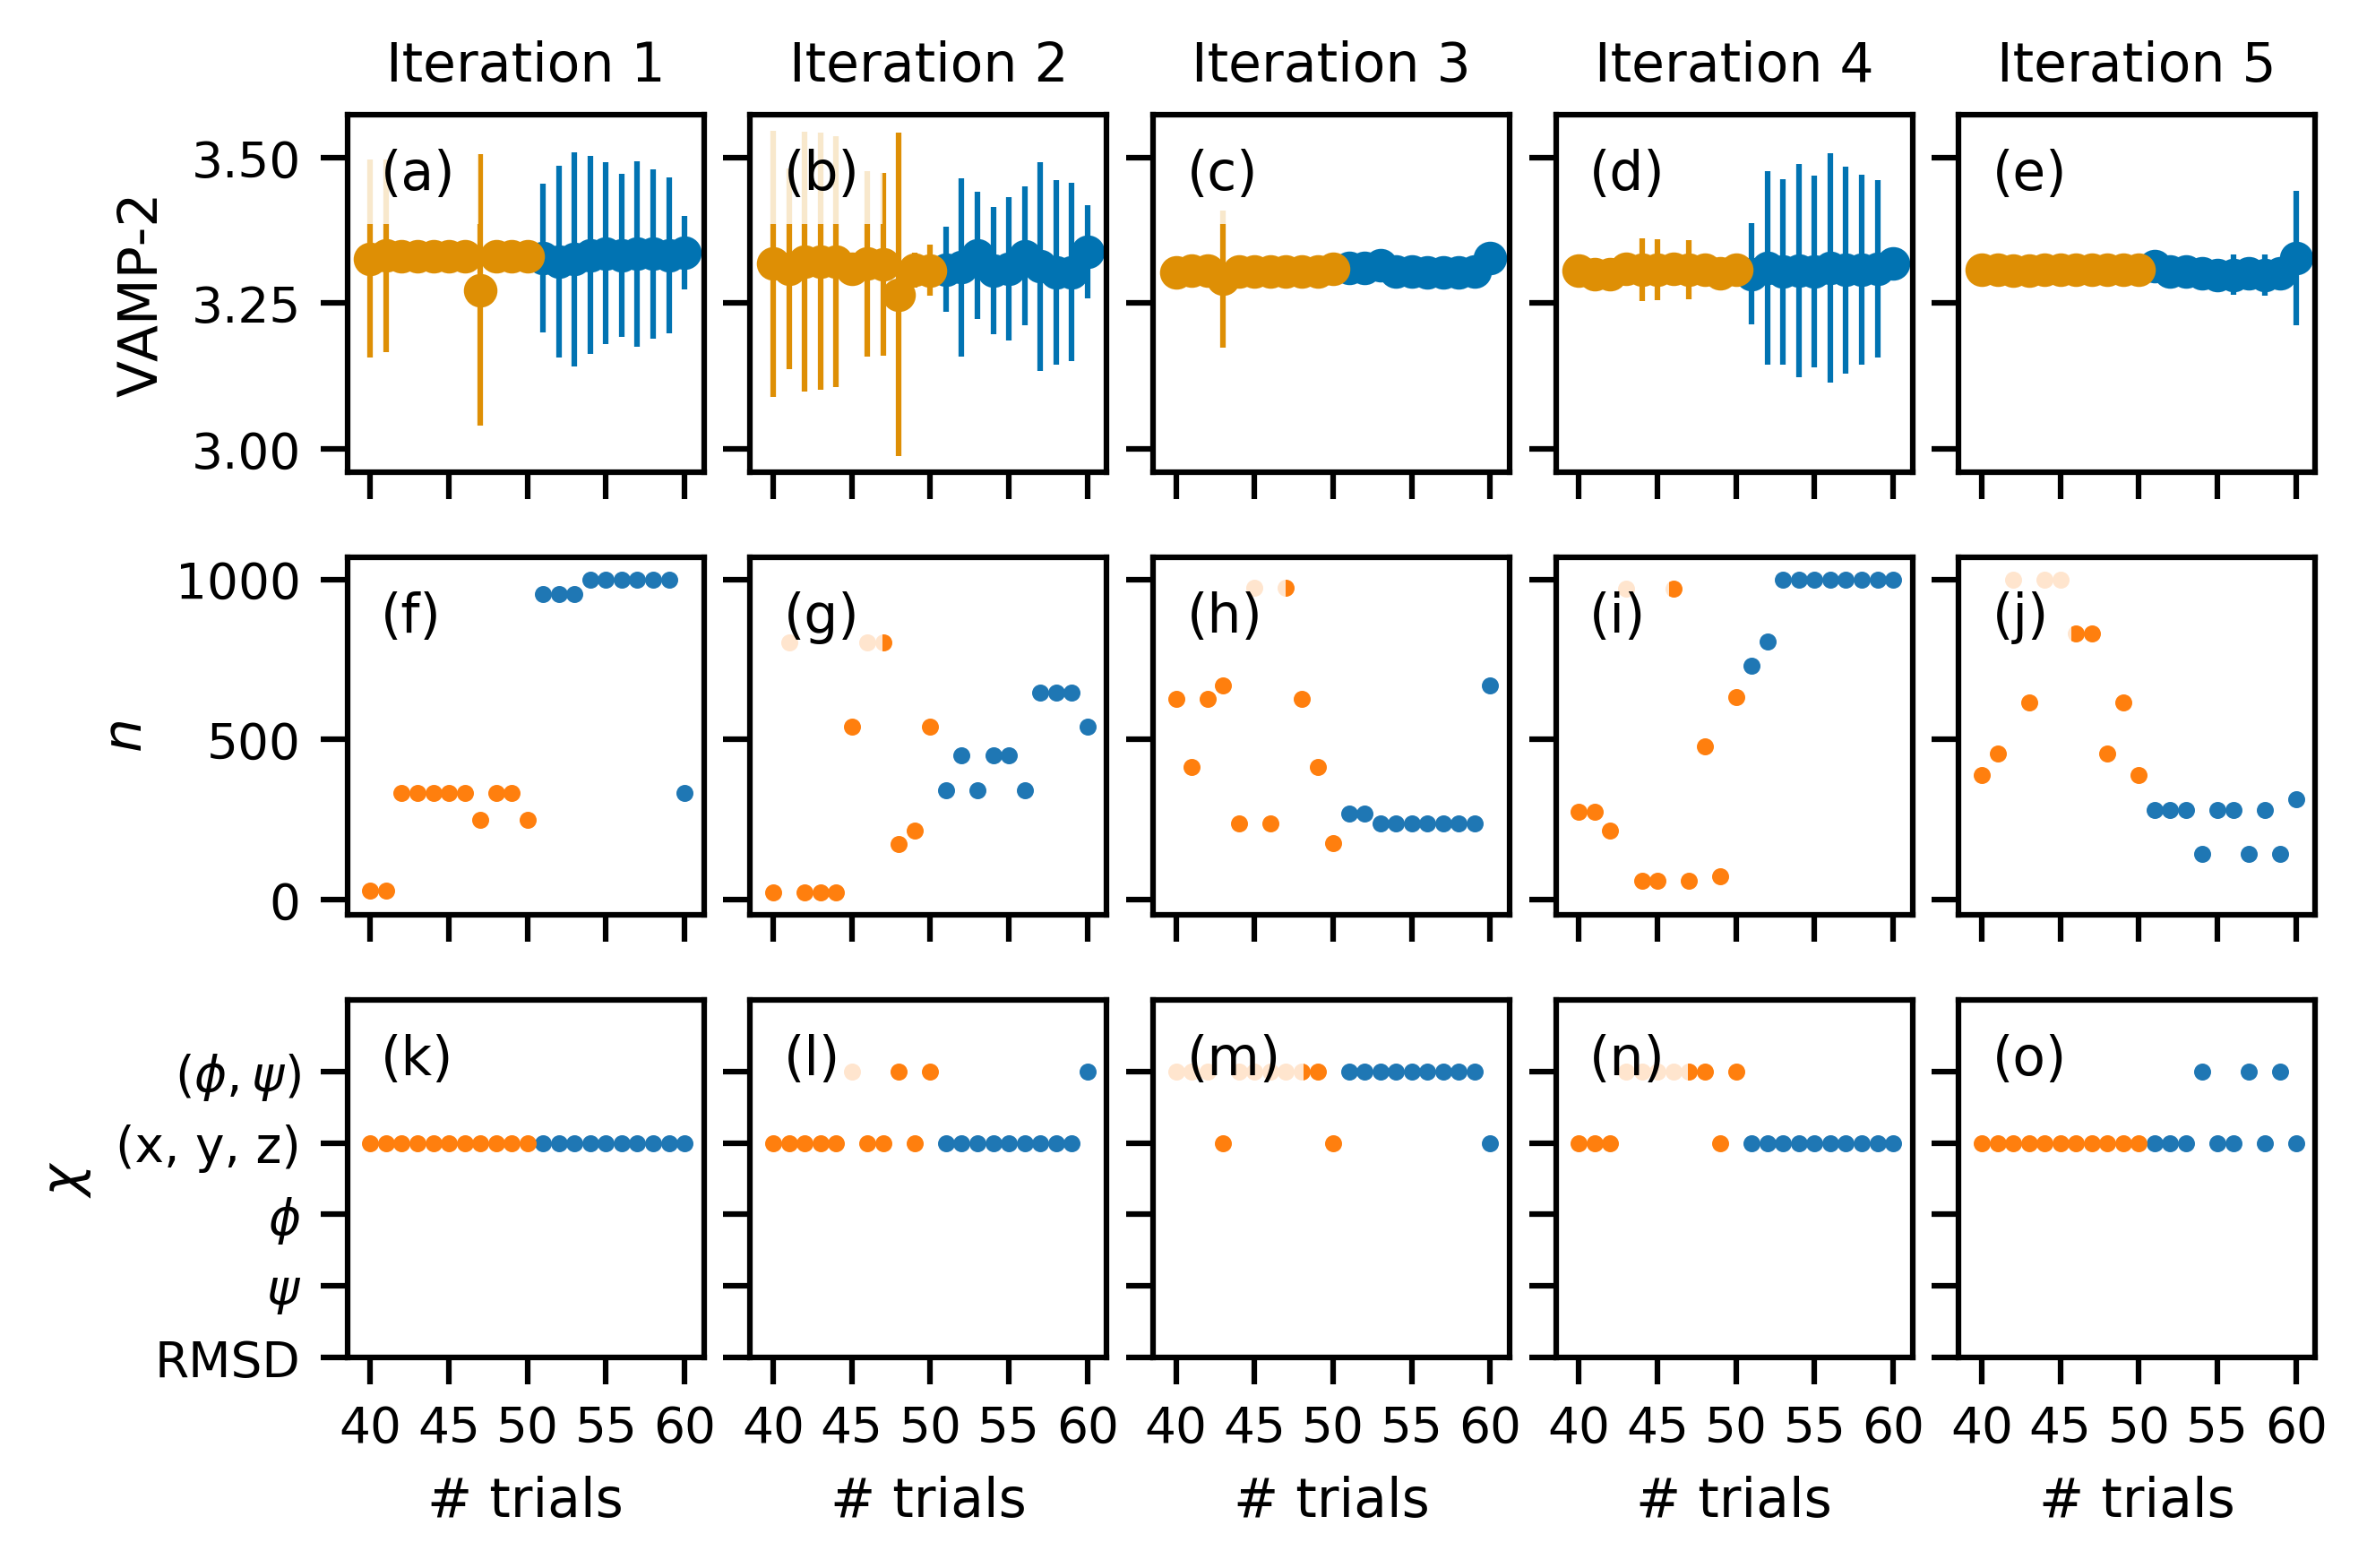
\includegraphics[width=0.8\linewidth]{chapters/msm_optimization/figures/ala1_opt_traj_start_obs_50.png}}
\end{figure}

The maximum of the response surface \emph{at the trial values} gives the optimum hyperparameters incorporating uncertainty and making full use of all the trial information. For alanine dipeptide the optimum hyper-parameters (using the GPR described in section \ref{subsubsec:ala_rsm}) these parameter are shown in in table xxx.  Given the large amount of sampling required to reach these values, a natural question to ask is: ``could we have arrived at these values with less sampling through optimization''? 

In order to answer this question an appropriate number of seed trial observations had to be determined first. The optimisation trajectories (i.e. the value of the incumbent and the associated predictors) are shown in figure \ref{fig:ala_opt_traj} seeded with 30 trials (or 15 observations per predictor, panel \ref{fig:ala_opt_traj_30} and 50 trials (or 25 observations per predictor, panel \ref{fig:ala_opt_traj_50}), and repeated five times to get a sense of the variation between optimisation trajectories. Each optimisation trajectory consisted of 10 steps of Bayesian optimisation (the blue points) but the figure also shows the trajectory calculated using the randomly sampled trials for comparison (the orange points). The input transformation and kernel function used were the same as those used on the full trial data set. In principle these GPR modelling choices should be determined independently for each data set but given the simplicity of the response surface it was deemed unnecessary for this system. With 30 seed trials, the incumbent trajectories of iteration 2, 3, \& 5 decreased, while for all iterations seeded with 50 seed trials \ref{fig:ala_opt_traj} the incumbent trajectories remained constant or increased. 50 seed trials, or 25 observations per predictor were therefore deemed appropriate. 

There are a number of observations of the optimisation trajectories which reflect on the alanine dipeptide response surface described in section \ref{subsubsec:ala_rsm} and the usefulness of Bayesian optimisation for this system. First, the incumbent trajectories clearly show that Bayesian optimisation does not increase the value of the incumbent. This is likely a reflection of the simple nature of the response surface and the irrelevance of the number of cluster centres. Second, the response surface (in the search space domain tested) is bimodal with peaks at $\chi=(\phi, \psi)$ torsions and $(x, y, z)$ coordinates. This is reflected in the clear lack of substantive difference between the incumbent value in, for example, panels (a) and (c) with different values of $\chi$ in panels (k) an (m)  of figure \ref{fig:ala_opt_traj}. Third, the almost complete irrelevance of $n$ as a hyper-parameter is clearly shown in panels (f) to (j) in which $n \simeq 1000, 500 \& 100$ are arrived at with no clear difference in the value of the incumbent. Fourth, it is possible that with more optimisation steps it could be possible to arrive at the maximum of the response surface with less seed trial observations. While this is a possibility, the fact that Bayesian optimisation is an inherently serial algorithm, while random sampling is embarrassingly parallel, it was considered more wall-time efficient (if not CPU-time efficient) to err on the side of more random seed trial data and less optimisation steps. 

% \begin{figure}
%     \centering
%     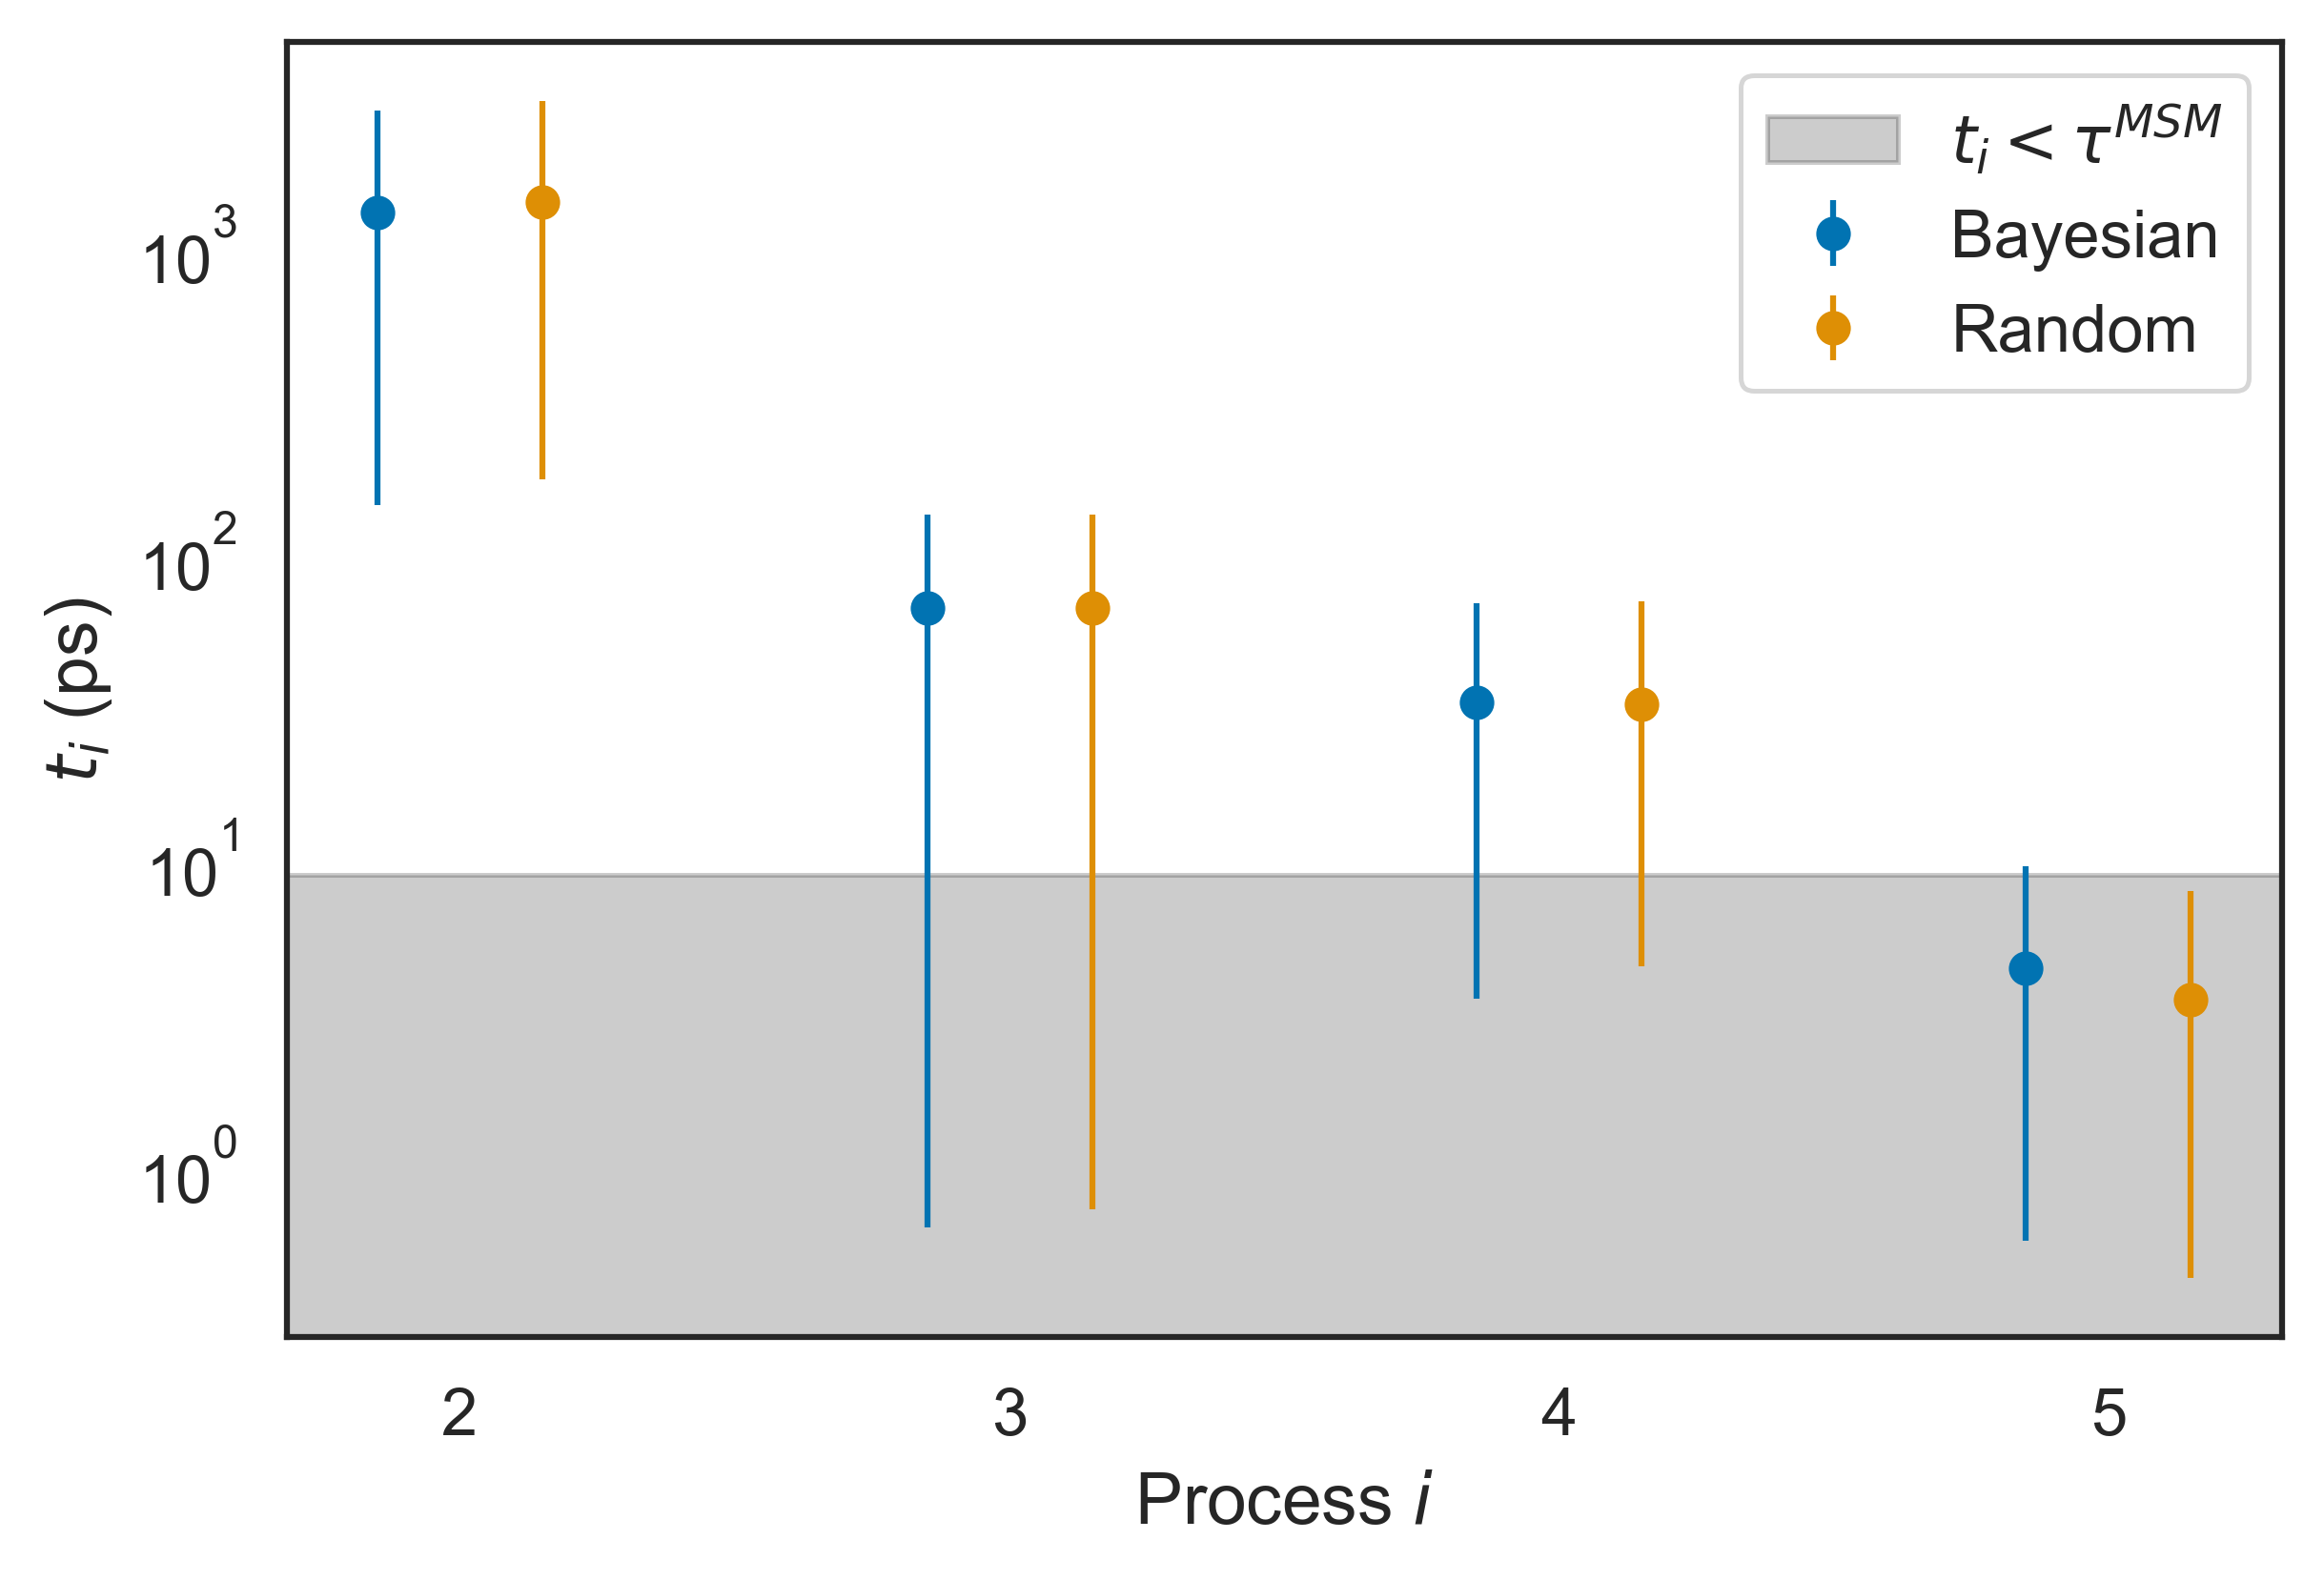
\includegraphics[width=0.8\linewidth]{chapters/msm_optimization/figures/ala1_opt_comparison.png}
%     \caption{Caption}
%     \label{fig:ala1_best_msm_ts}
% \end{figure}
% \begin{figure}
%     \centering
%     \begin{subfigure}[b]{0.3\textwidth}
%         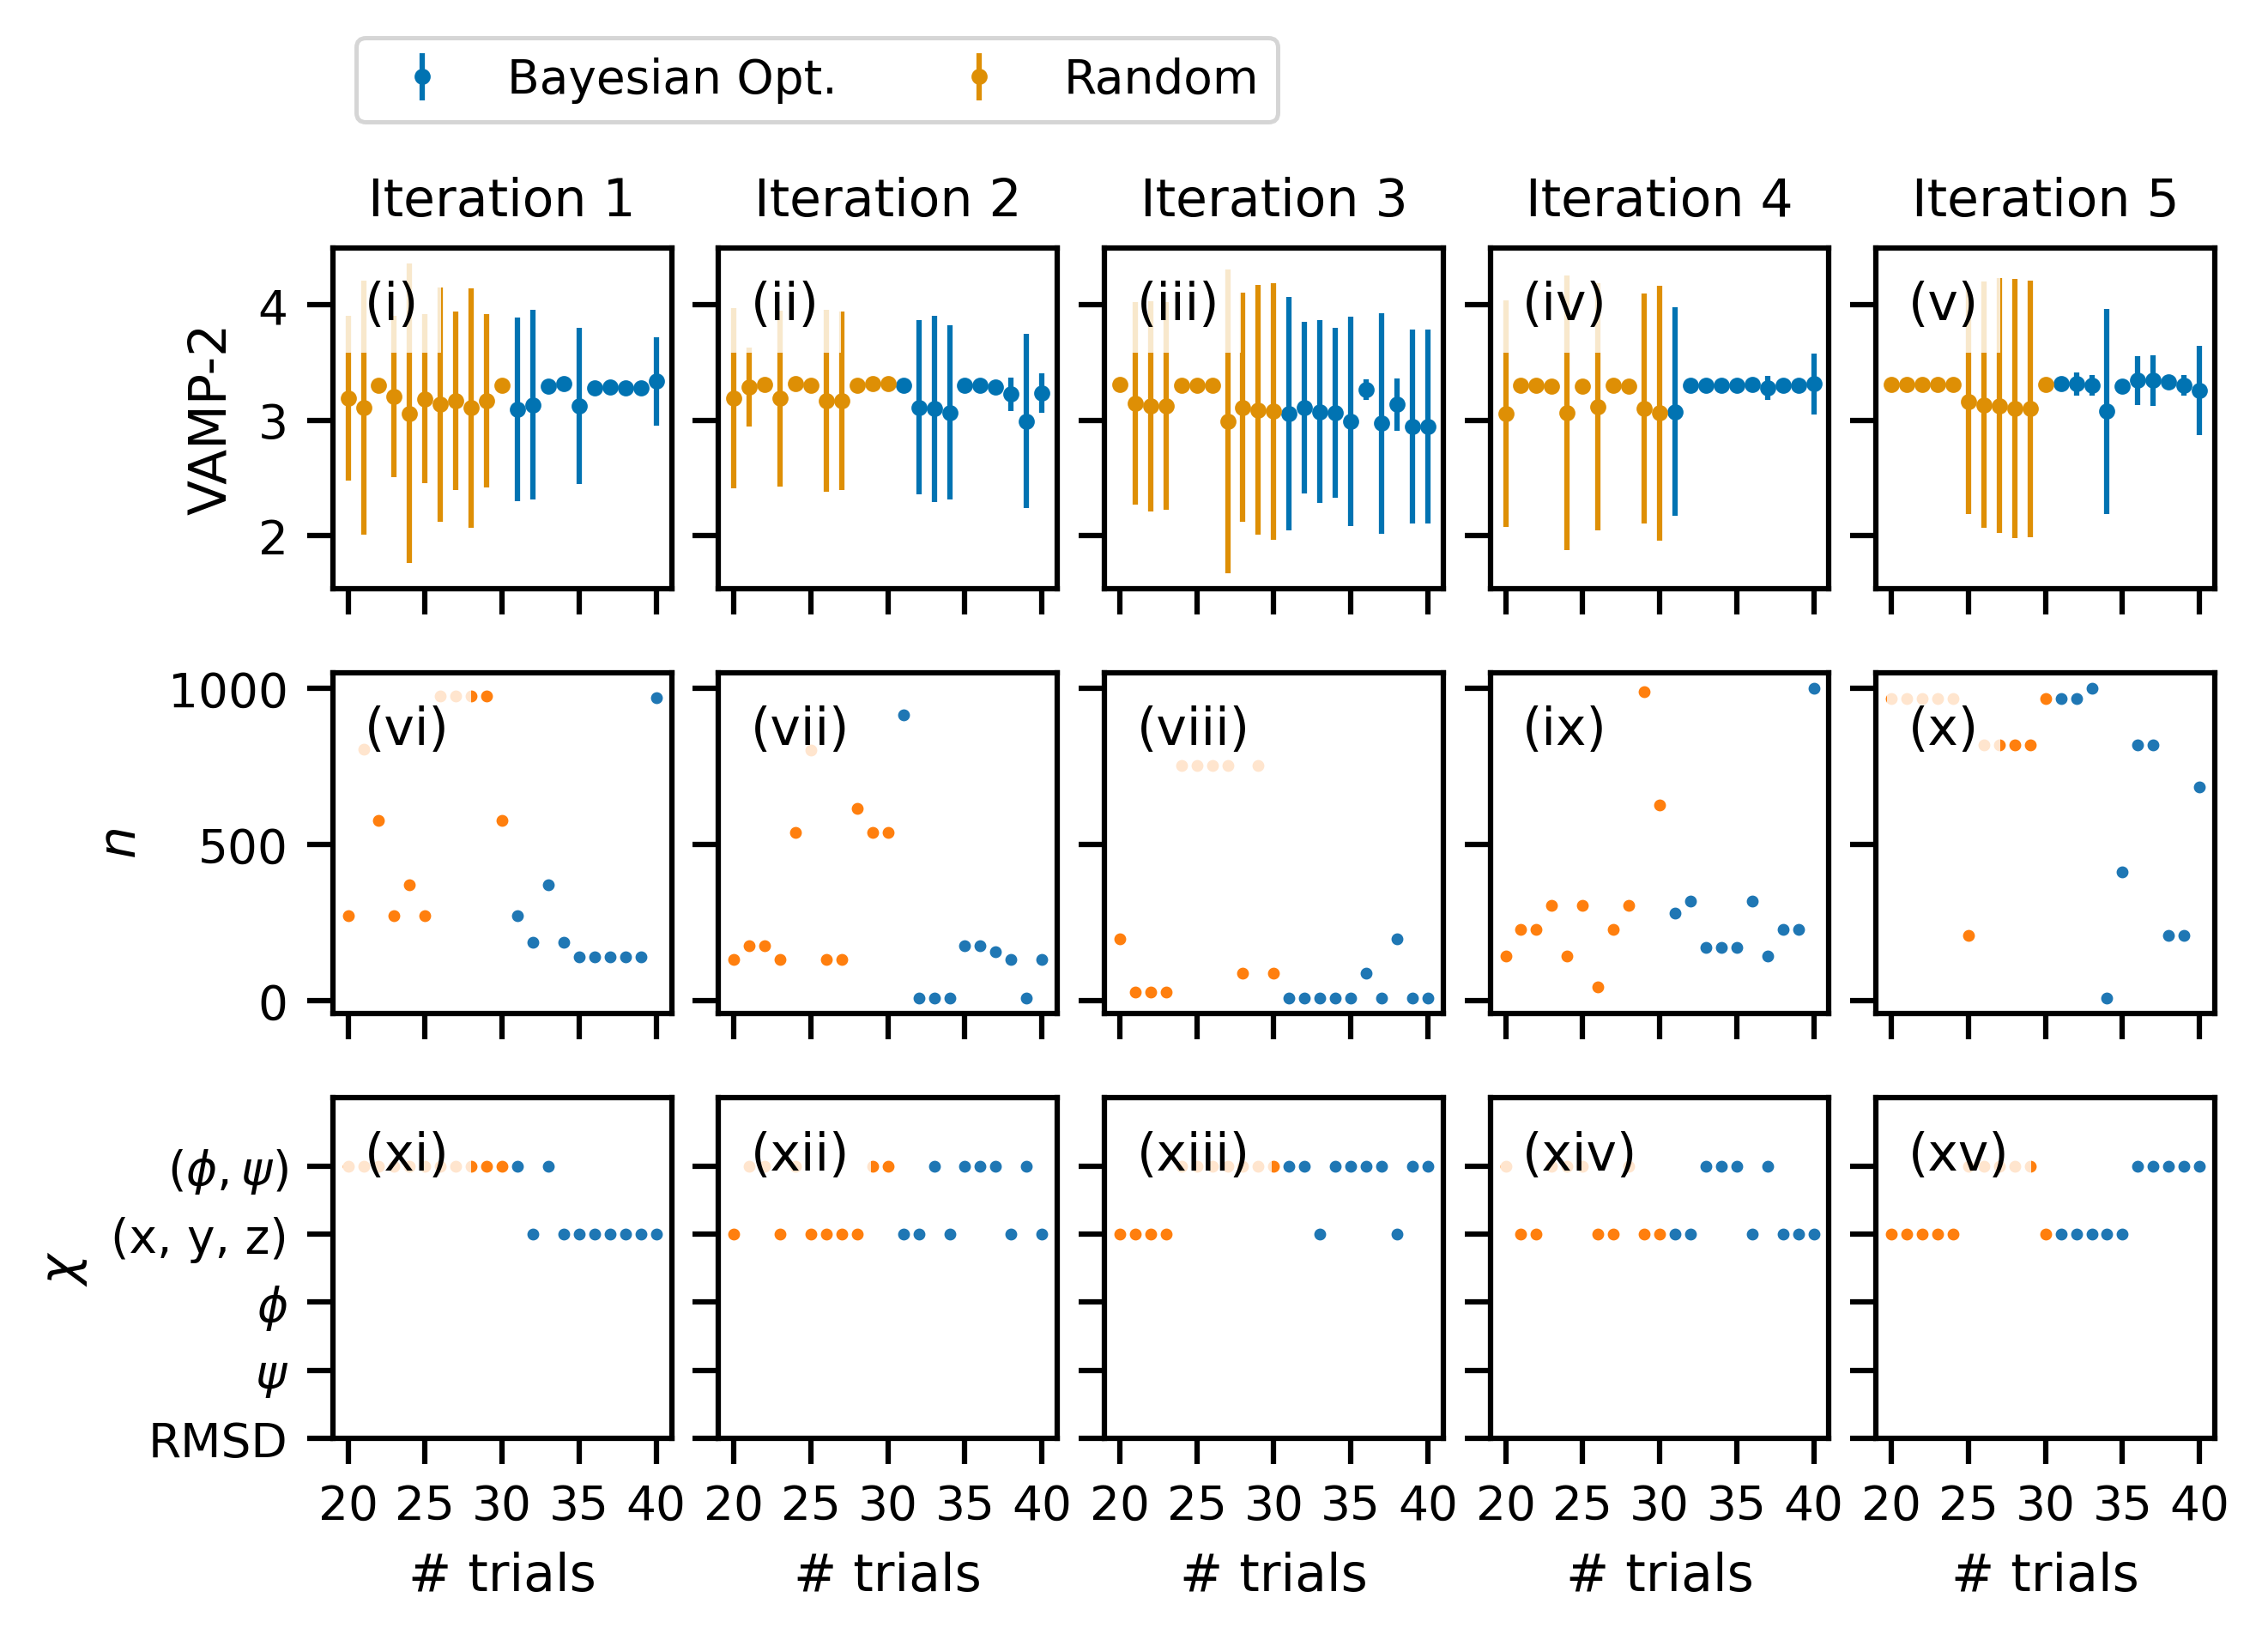
\includegraphics[width=\textwidth]{chapters/msm_optimization/figures/ala1_opt_traj_start_obs_30.png}
%         \caption{A gull}
%         \label{fig:gull}
%     \end{subfigure}
%     ~ %add desired spacing between images, e. g. ~, \quad, \qquad, \hfill etc. 
%       %(or a blank line to force the subfigure onto a new line)
%     \begin{subfigure}[b]{0.3\textwidth}
%         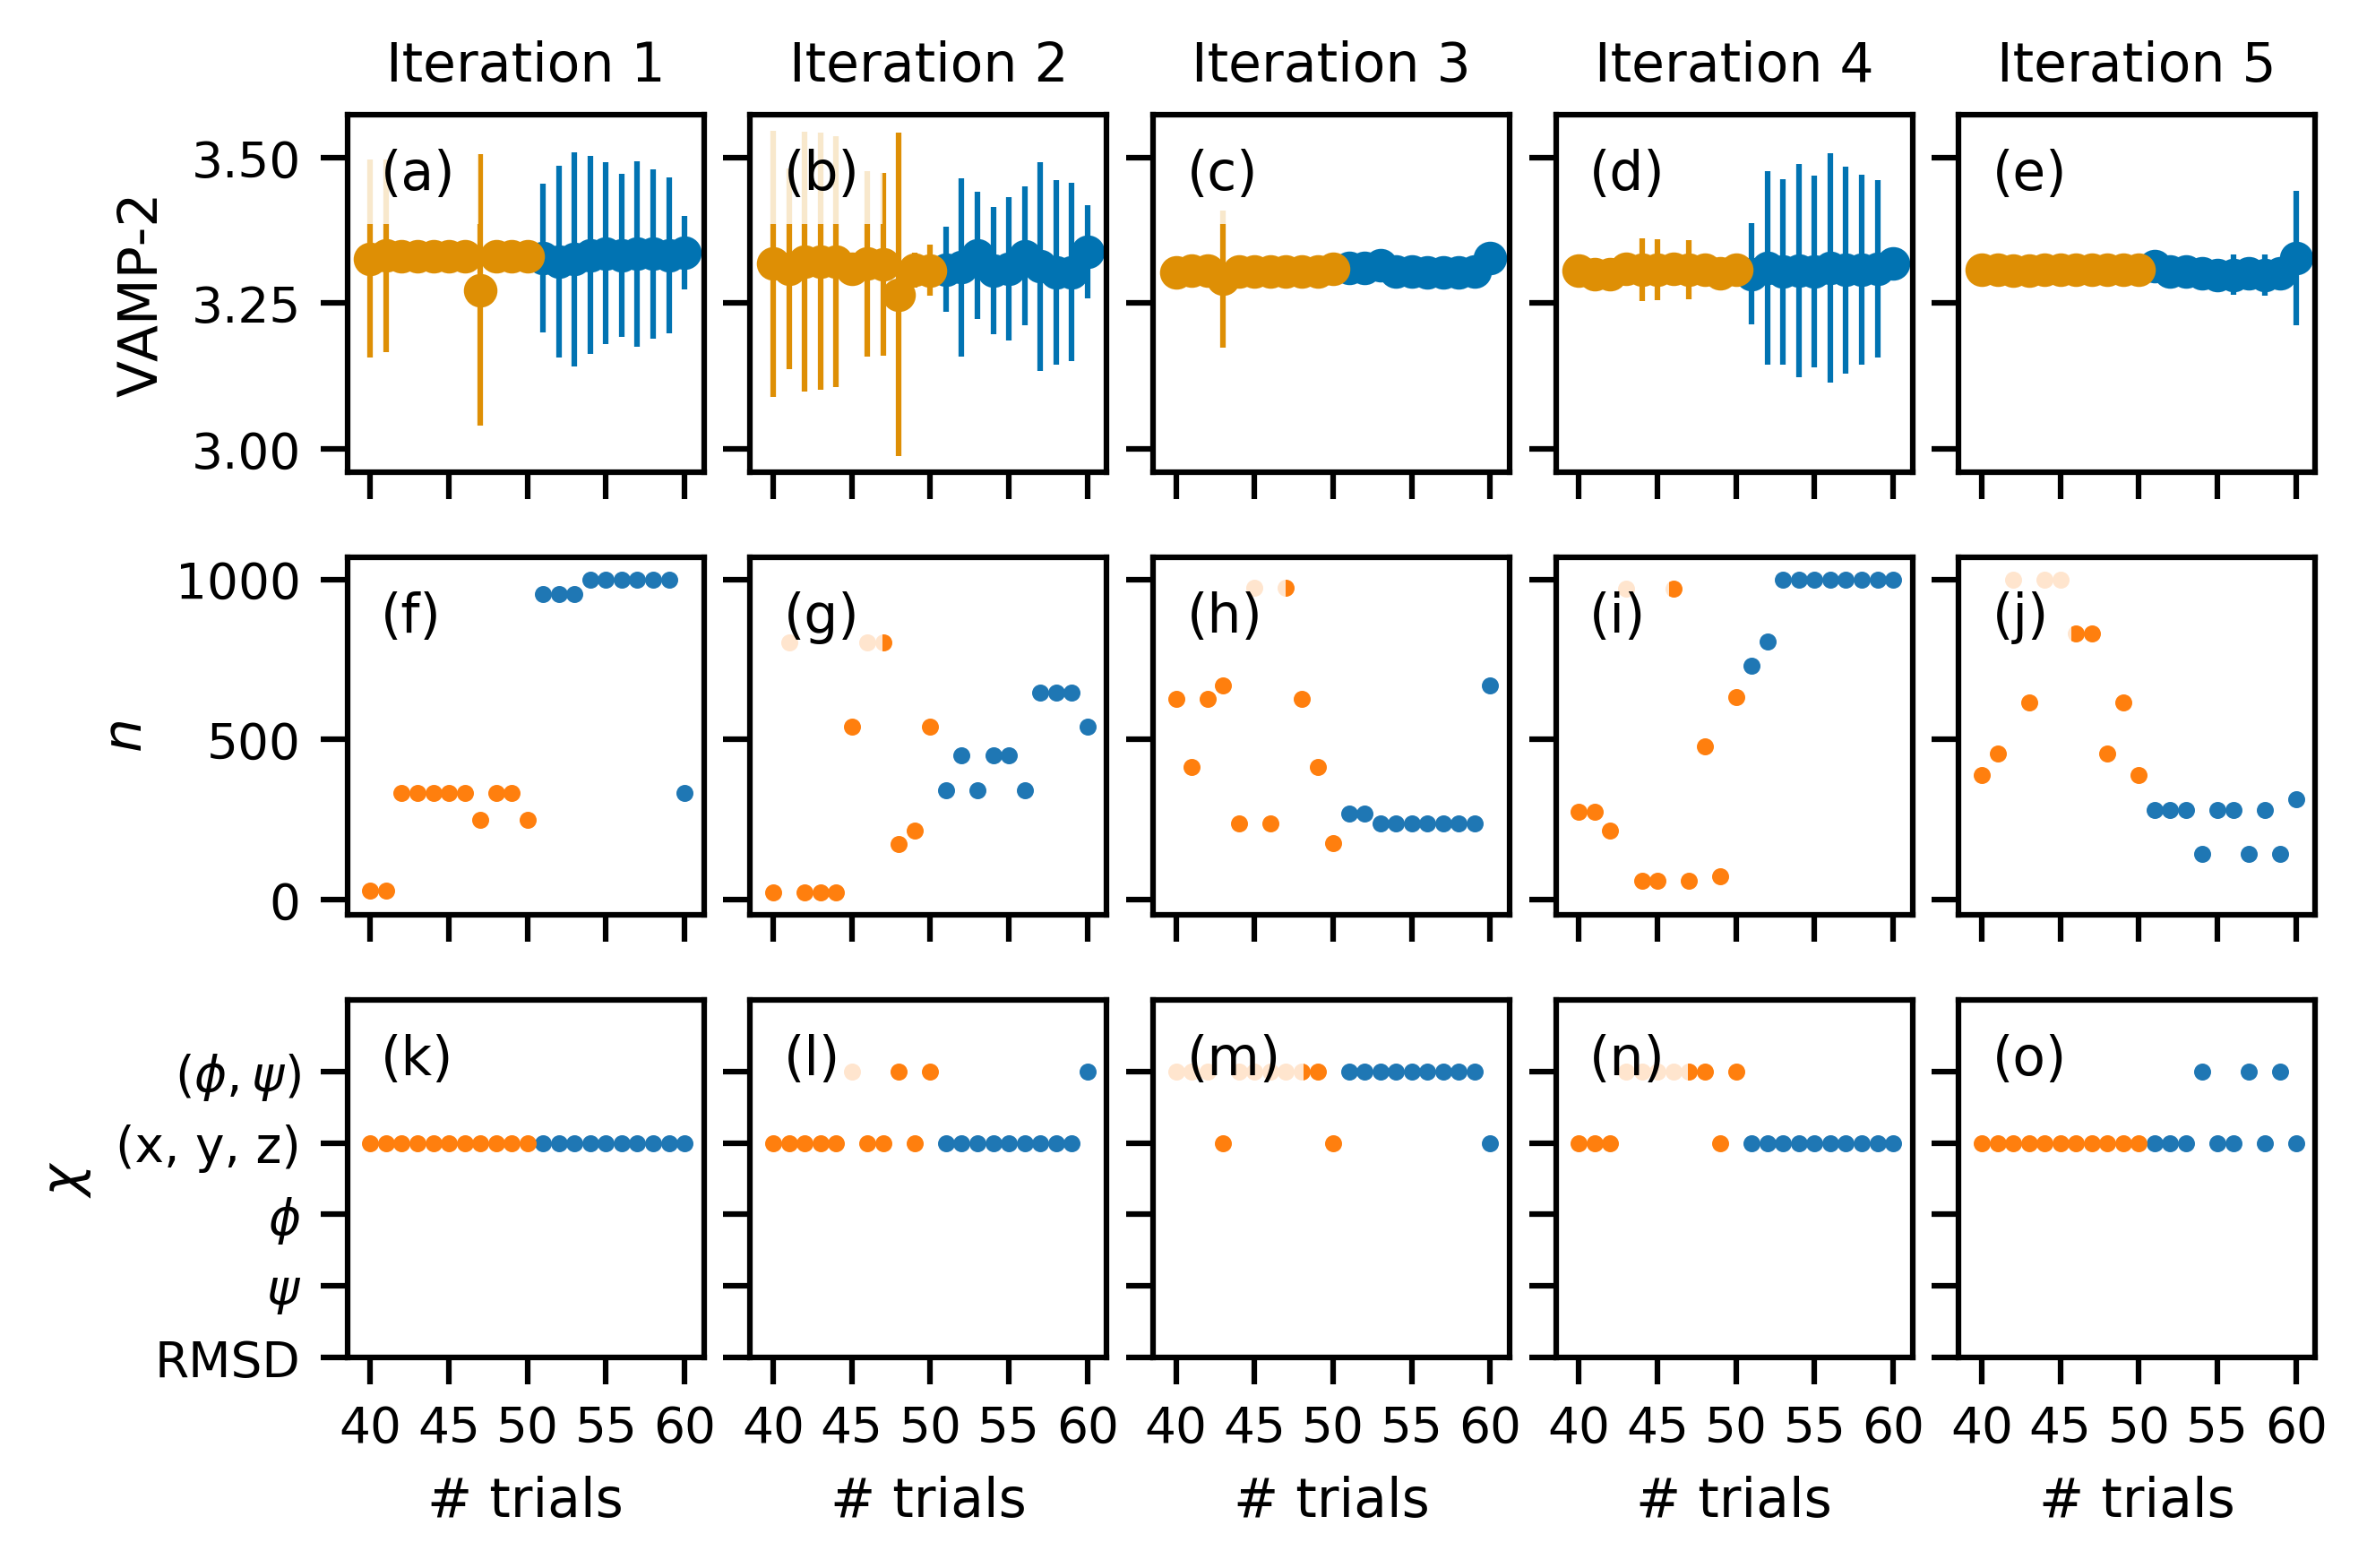
\includegraphics[width=\textwidth]{chapters/msm_optimization/figures/ala1_opt_traj_start_obs_50.png}
%         \caption{A tiger}
%         \label{fig:tiger}
%     \end{subfigure}
%     ~ %add desired spacing between images, e. g. ~, \quad, \qquad, \hfill etc. 
%     %(or a blank line to force the subfigure onto a new line)
% \end{figure}

\subsection{Aromatic Amine Dehydrogenase}\label{subsec:aadh}
\subsubsection{Response surface}\label{subsubsec:aadh_rsm}
The average MSM response for each trial are shown in figure \ref{fig:aad_train_test}, shown grouped in panels according to the value $\chi$,  and ranked according to mean test response (shown in blue). The panels are ordered according to their average of the test responses and the mean response on the training data is shown in orange. There is clear range of response values in the range $2 < VAMP-2 < 4$ with the $(\phi, \psi, \chi)$ torsions and the interatomic distances feature ( $\left|\mathbf{r}_{1}-\mathbf{r}_{2}\right|$) both performing the best out of the five features. 

The response surface as a function of the feature, $\chi$, TICA lag time, $\tau$, number of TICA components retains $m$, and the number of cluster centres, $n$ was estimated with a MML GPR. Model selection on the kernel and input transformation revealed an exponential kernel (equation \ref{eqn:kern_exp}) and a linear input transformation were most appropriate, with an MSLL of $-0.01298$ and a SMSE of $0.3087$, see table \ref{tab:aadh_rsm_metrics_all_data} for the other model selection metrics. A more intuitive assessment of the fit of the can be found in figure  \ref{fig:aadh_rsm_fit} which shows the observed and predicted values for each feature. There is clearly a good fit for all the features except for the $(\phi, \psi, \chi)$ torsions where the predicted values are slightly under (over) estimated for the highest (lowest) values with this feature. 

The RMSD feature was left out of the response surface because the $\tau$ and $m$ hyper-parameters do not apply and this poses problems for incorporating this feature into the response surface modelled by a GP.  While this is a problem in general for this method, the poor performance of RMSD as a feature both here, in alanine dipeptide mean that this does not impact many of the conclusions that can be drawn. 

The multidimensional nature of the response surface poses problems for visualisation. However, calculating the hyper-parameter relevance before attempting to do this can help by guiding in the displayed granularity of the inputs. Figure \ref{fig:aadh_relevance} shows the relevance for the levels of $\chi$ (in blue) and the remaining hyper-parameters (orange) and figure \ref{fig:aadh_rsm} show the response surface. $\tau$ and $m$ are the two highest relevance features so the response surface is shown as a 2D heat map with $\tau$ on the vertical and $m$ on the horizontal axis. Only odd values of $m$ are shown give the slightly lower relevance of this feature. The number of cluster features is again the lowest relevance feature and so heat maps for only two value of $n$ are shown: the value at the maximum ($n=207$ although the value displayed was rounded to $210$) and $n=1000$. With only four features, it is relatively simple to show the response surface for each of them. As all features are relatively low relevance their response surfaces are expected to be very similar. The maximum of the response surface is shown highlighted in white and the corresponding values are shown in table \ref{tab:aadh_opt_results}. 

In order to test the convergence of this maximum, 50 steps of Bayesian optimisation was performed seeding the algorithm with all $361$ trials. This resulted in a small, $\SI{0.5}{\percent}$ improvement in the response and small changes in the optimal hyper-parameters.  In order to see whether this maximum could be reached with a few number of trials, five subsets of the trial data set, with 100 observations, were optimized with 50 steps of Bayesian optimisation. The response surface kernel and input transformations were determined by the GP model selection methods described in section \ref{subsec:rsm}. 

The incumbent trajectories are shown in are shown in figure \ref{fig:aadh_opt_traj_d}. The maximum of the response surface with $N=361$ randomly sampled trials are shown as orange lines, and the maximum of the surface with an $N=410$ trials including the $50$ steps of Bayesian optimisation are shown as blue lines.  The figure clearly shows that the Bayesian optimisation does not improve the maximum of the response nor does it greatly affect the value of the optimal hyperparameters. The uncertainty in the incumbent decreased in three of the five incumbent trajectories however.  The final and starting values of the optimisation trajectories are tabulated in table \ref{tab:aadh_opt_results}. 

These optimisation results clearly indicate that the response surface is reasonably well converged for even $100$ trials and that the number of seed trials determined from alanine dipeptide was not applicable here.  




\begin{figure}[ht]
    \centering
    \caption{Relevance of MSM for active site D}
    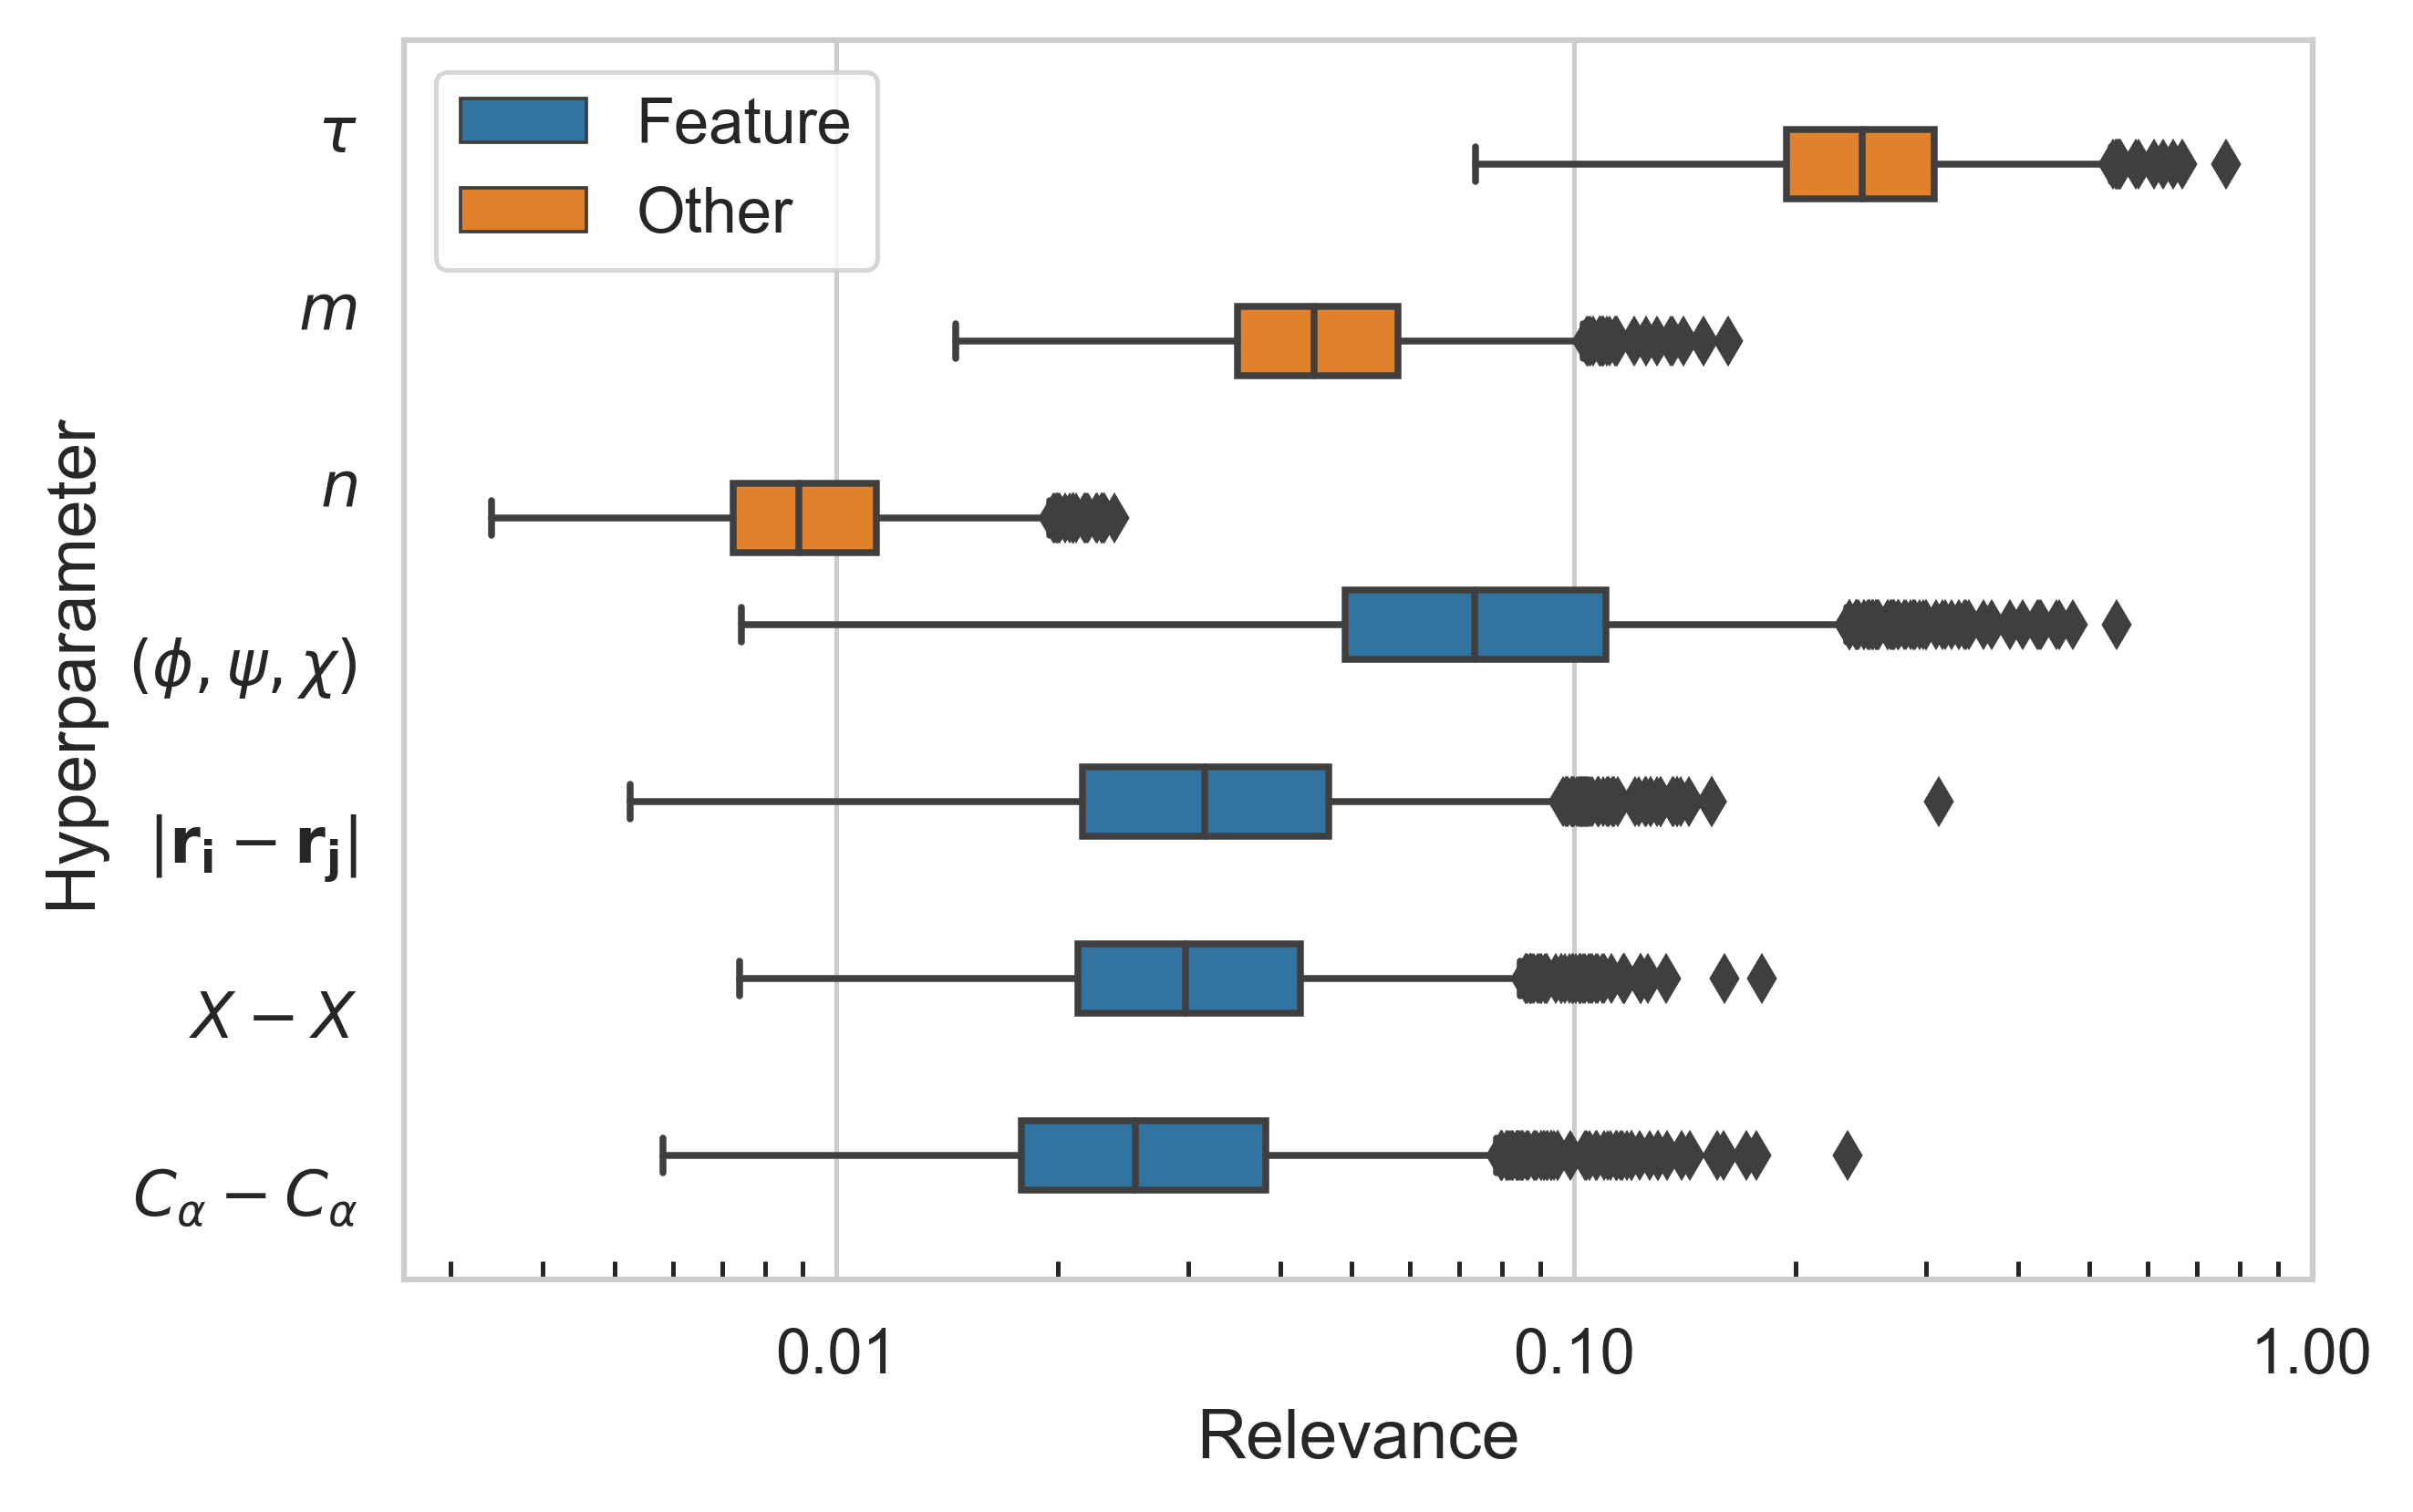
\includegraphics[width=0.8\textwidth]{chapters/msm_optimization/figures/AADH_relevance_d.png}
    
    \label{fig:aadh_relevance}
\end{figure}

\begin{figure}[ht]
    \centering
    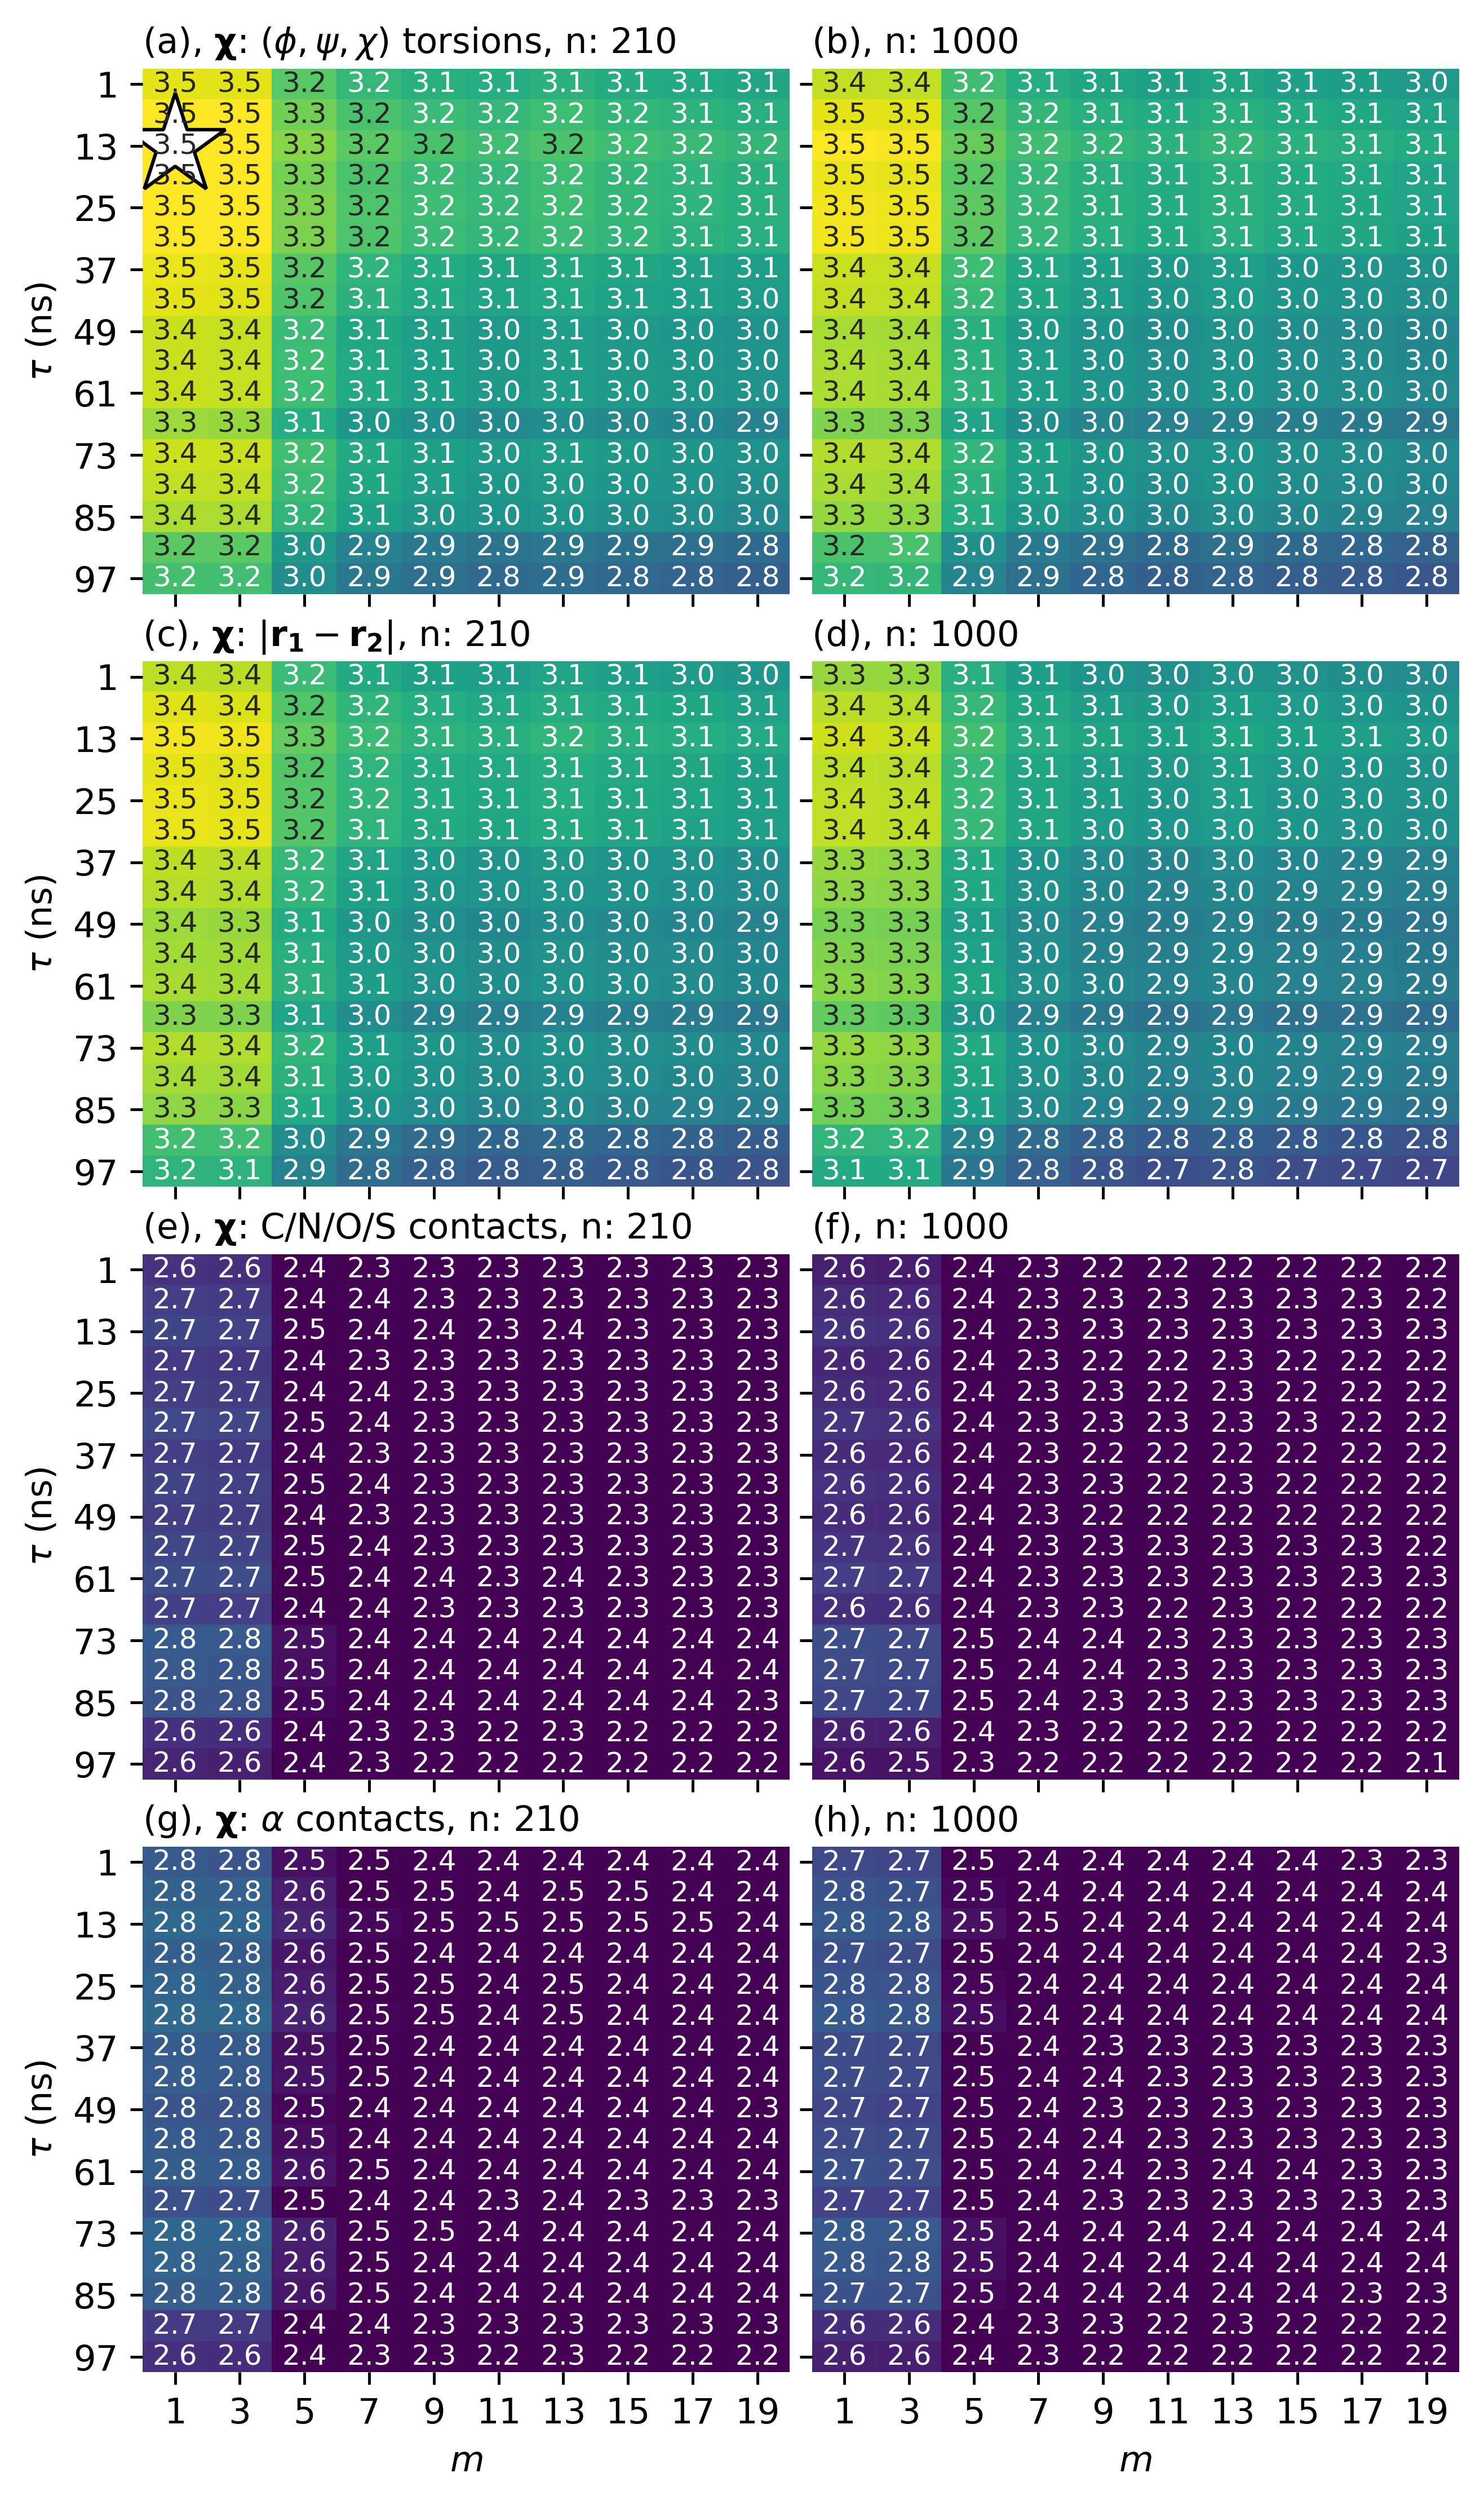
\includegraphics[width=0.8\textwidth]{chapters/msm_optimization/figures/aadh_response_surface_d.png}
    \caption{Caption}
    \label{fig:aadh_rsm}
\end{figure}

\begin{table}
    \centering
    \begin{tabular}{|l|l|r|r|r|l|r|r|r|}
    \hline
       Sampling &        Label &  Num. Trials & $\mu$ & $\sigma$ &                $\chi$ & $\tau$ & $m$ & $n$ \\
    \hline\hline
         Random &              & 361 &  3.54 & 0.20 &  $(\phi, \psi, \chi)$ &   12.5 &   1 & 207 \\
     Bayes Opt. &              &410 &  3.56 & 0.09 &  $(\phi, \psi, \chi)$ &   10.0 &   2 & 310 \\
     Bayes Opt. &  Iteration 0 &150 &  3.50 & 0.20 &  $(\phi, \psi, \chi)$ &    1.0 &   2 &  10 \\
     Bayes Opt. &  Iteration 1 &150 &  3.56 & 0.12 &  $(\phi, \psi, \chi)$ &    4.0 &   1 & 180 \\
     Bayes Opt. &  Iteration 2 &150 &  3.54 & 0.10 &  $(\phi, \psi, \chi)$ &    3.0 &   2 &  10 \\
     Bayes Opt. &  Iteration 3 &150 &  3.58 & 0.08 &  $(\phi, \psi, \chi)$ &    1.0 &   1 & 230 \\
     Bayes Opt. &  Iteration 4 &150 &  3.57 & 0.07 &  $(\phi, \psi, \chi)$ &    1.0 &   1 & 540 \\
    \hline
    \end{tabular}
    \caption{Caption}
    \label{tab:aadh_opt_results}
\end{table}

\begin{figure}
    \centering
    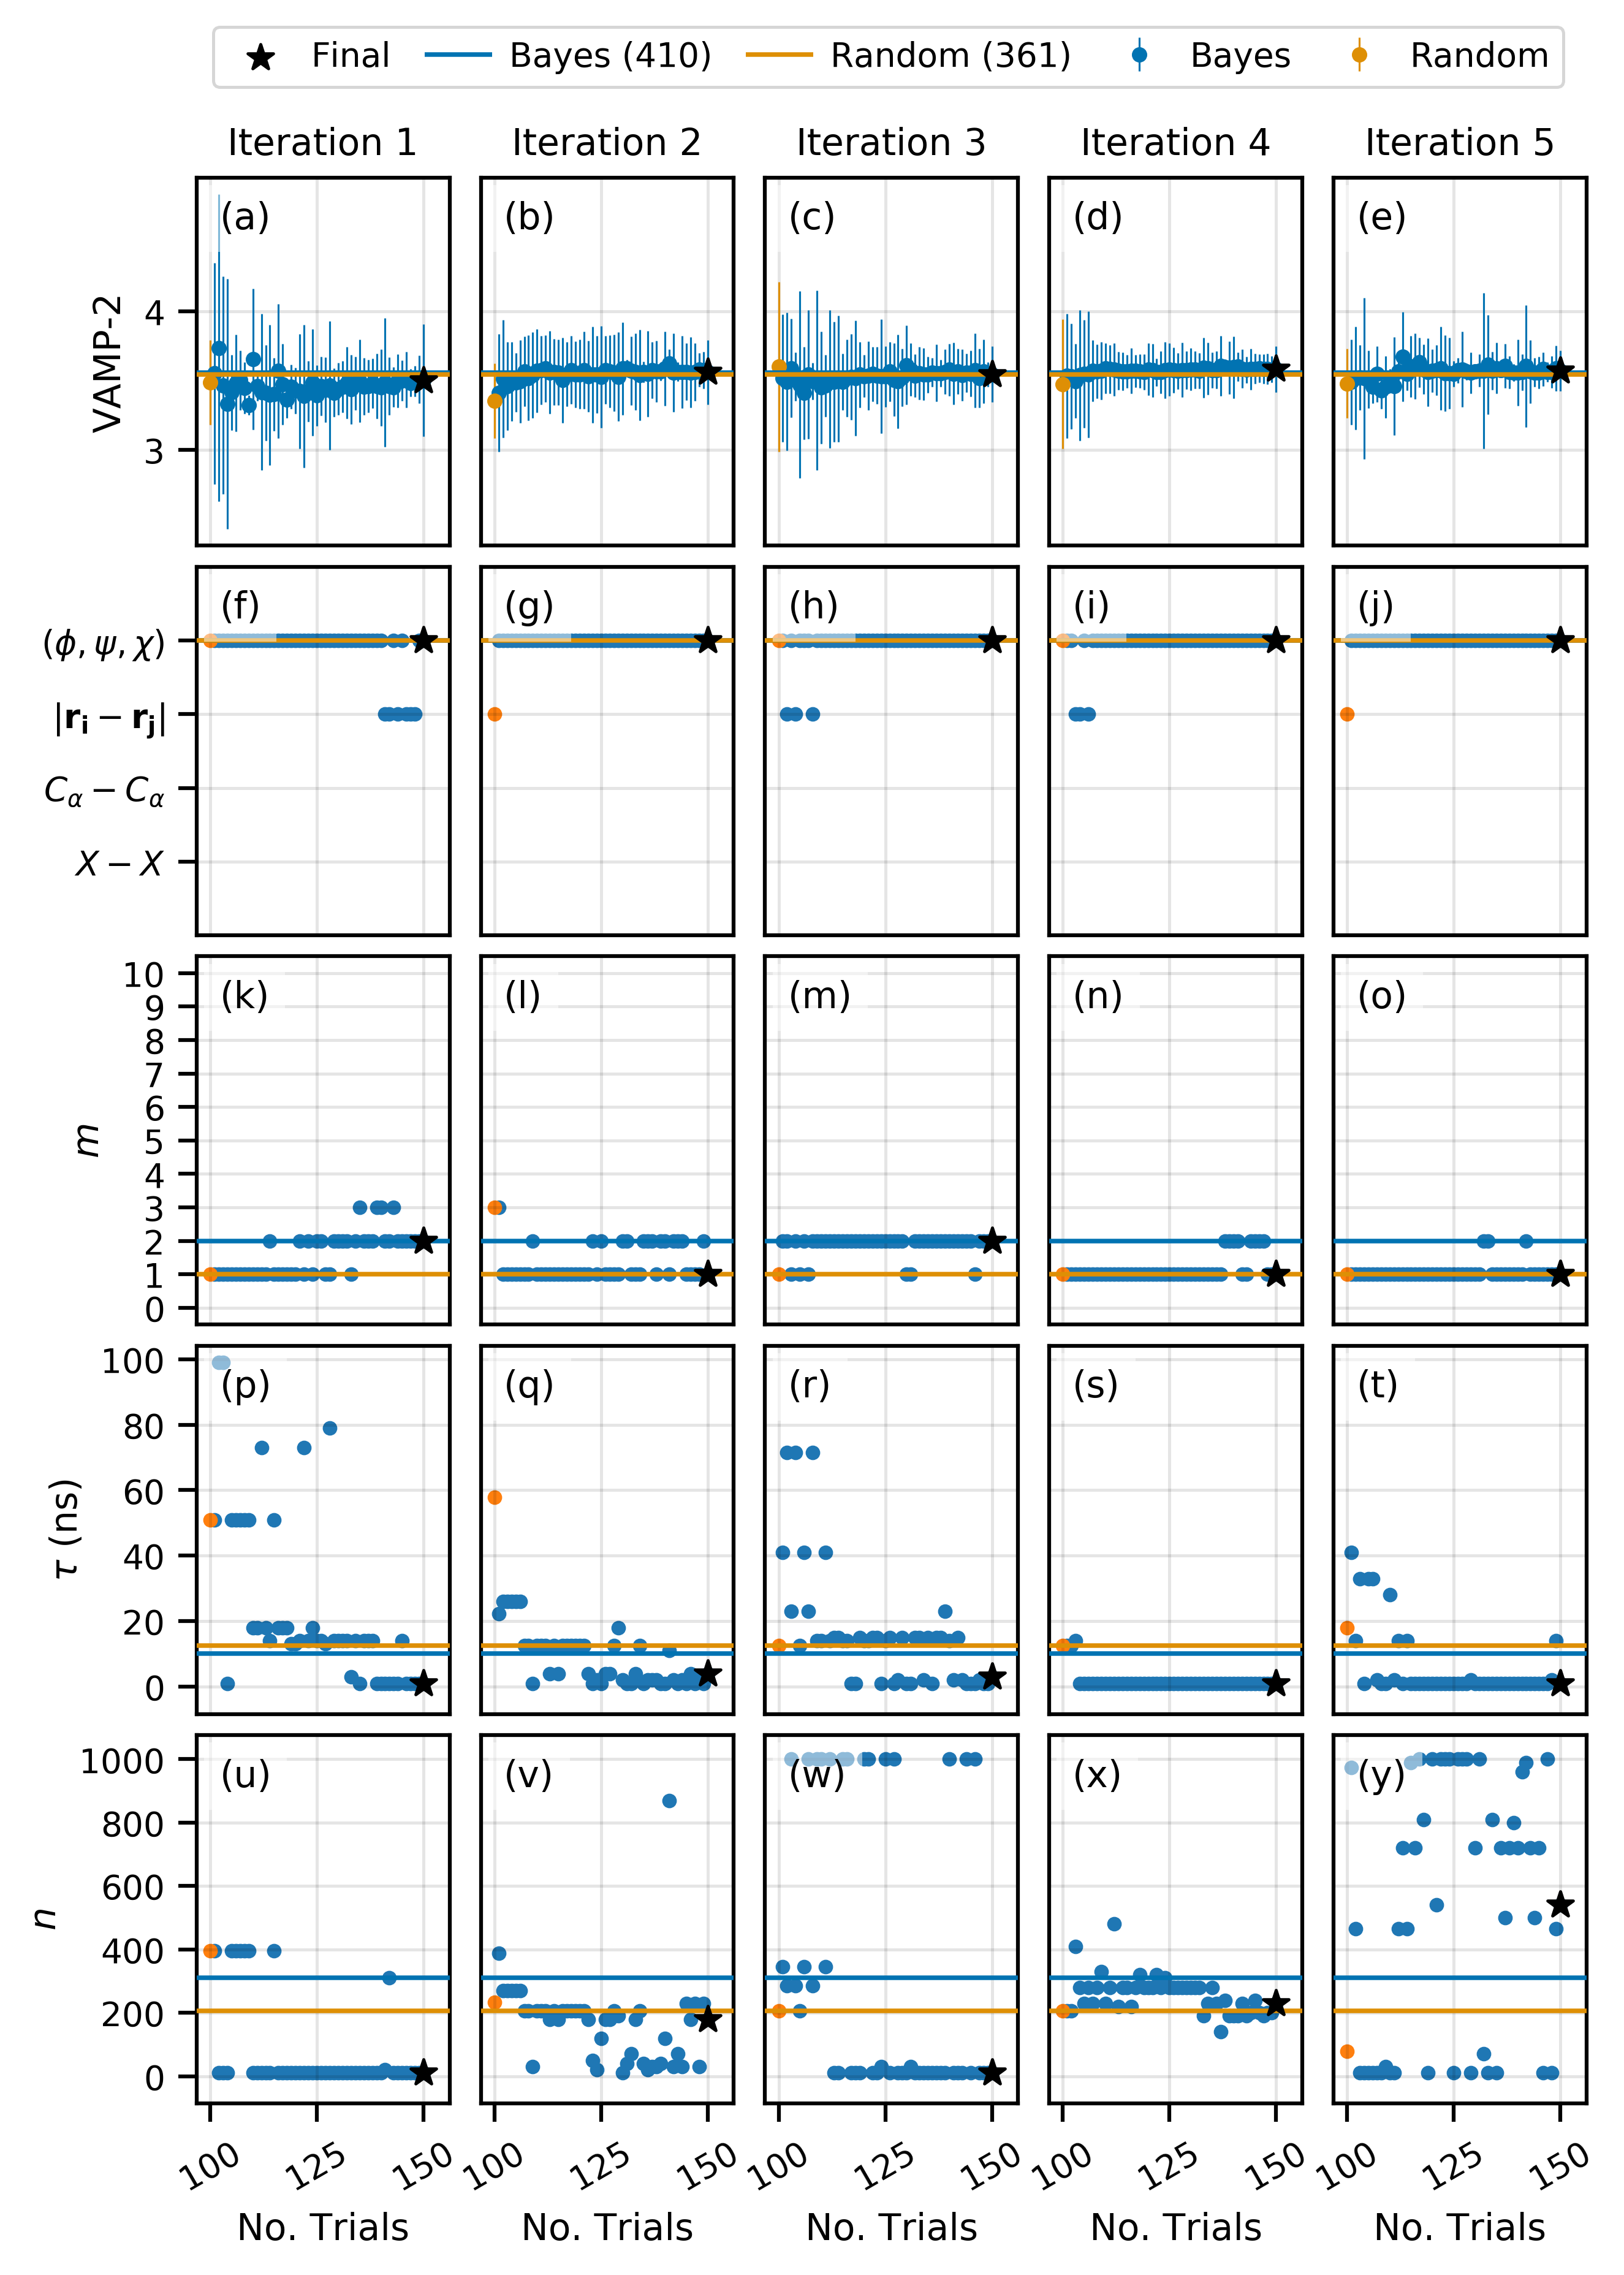
\includegraphics[width=0.8\textwidth]{chapters/msm_optimization/figures/aadh_opt_traj_act_s_d.png}
    \caption{Caption}
    \label{fig:aadh_opt_traj_d}
\end{figure}

\subsubsection{Response surface and MSM observables}

\begin{figure}[ht!]
    \centering
    \mycaption{AADH implied timescales}\label{fig:aadh_its}
    \subtop[$1<\tau^{MSM}<\SI{5}{\nano\second}$ \label{fig:aadh_its_short}]{
        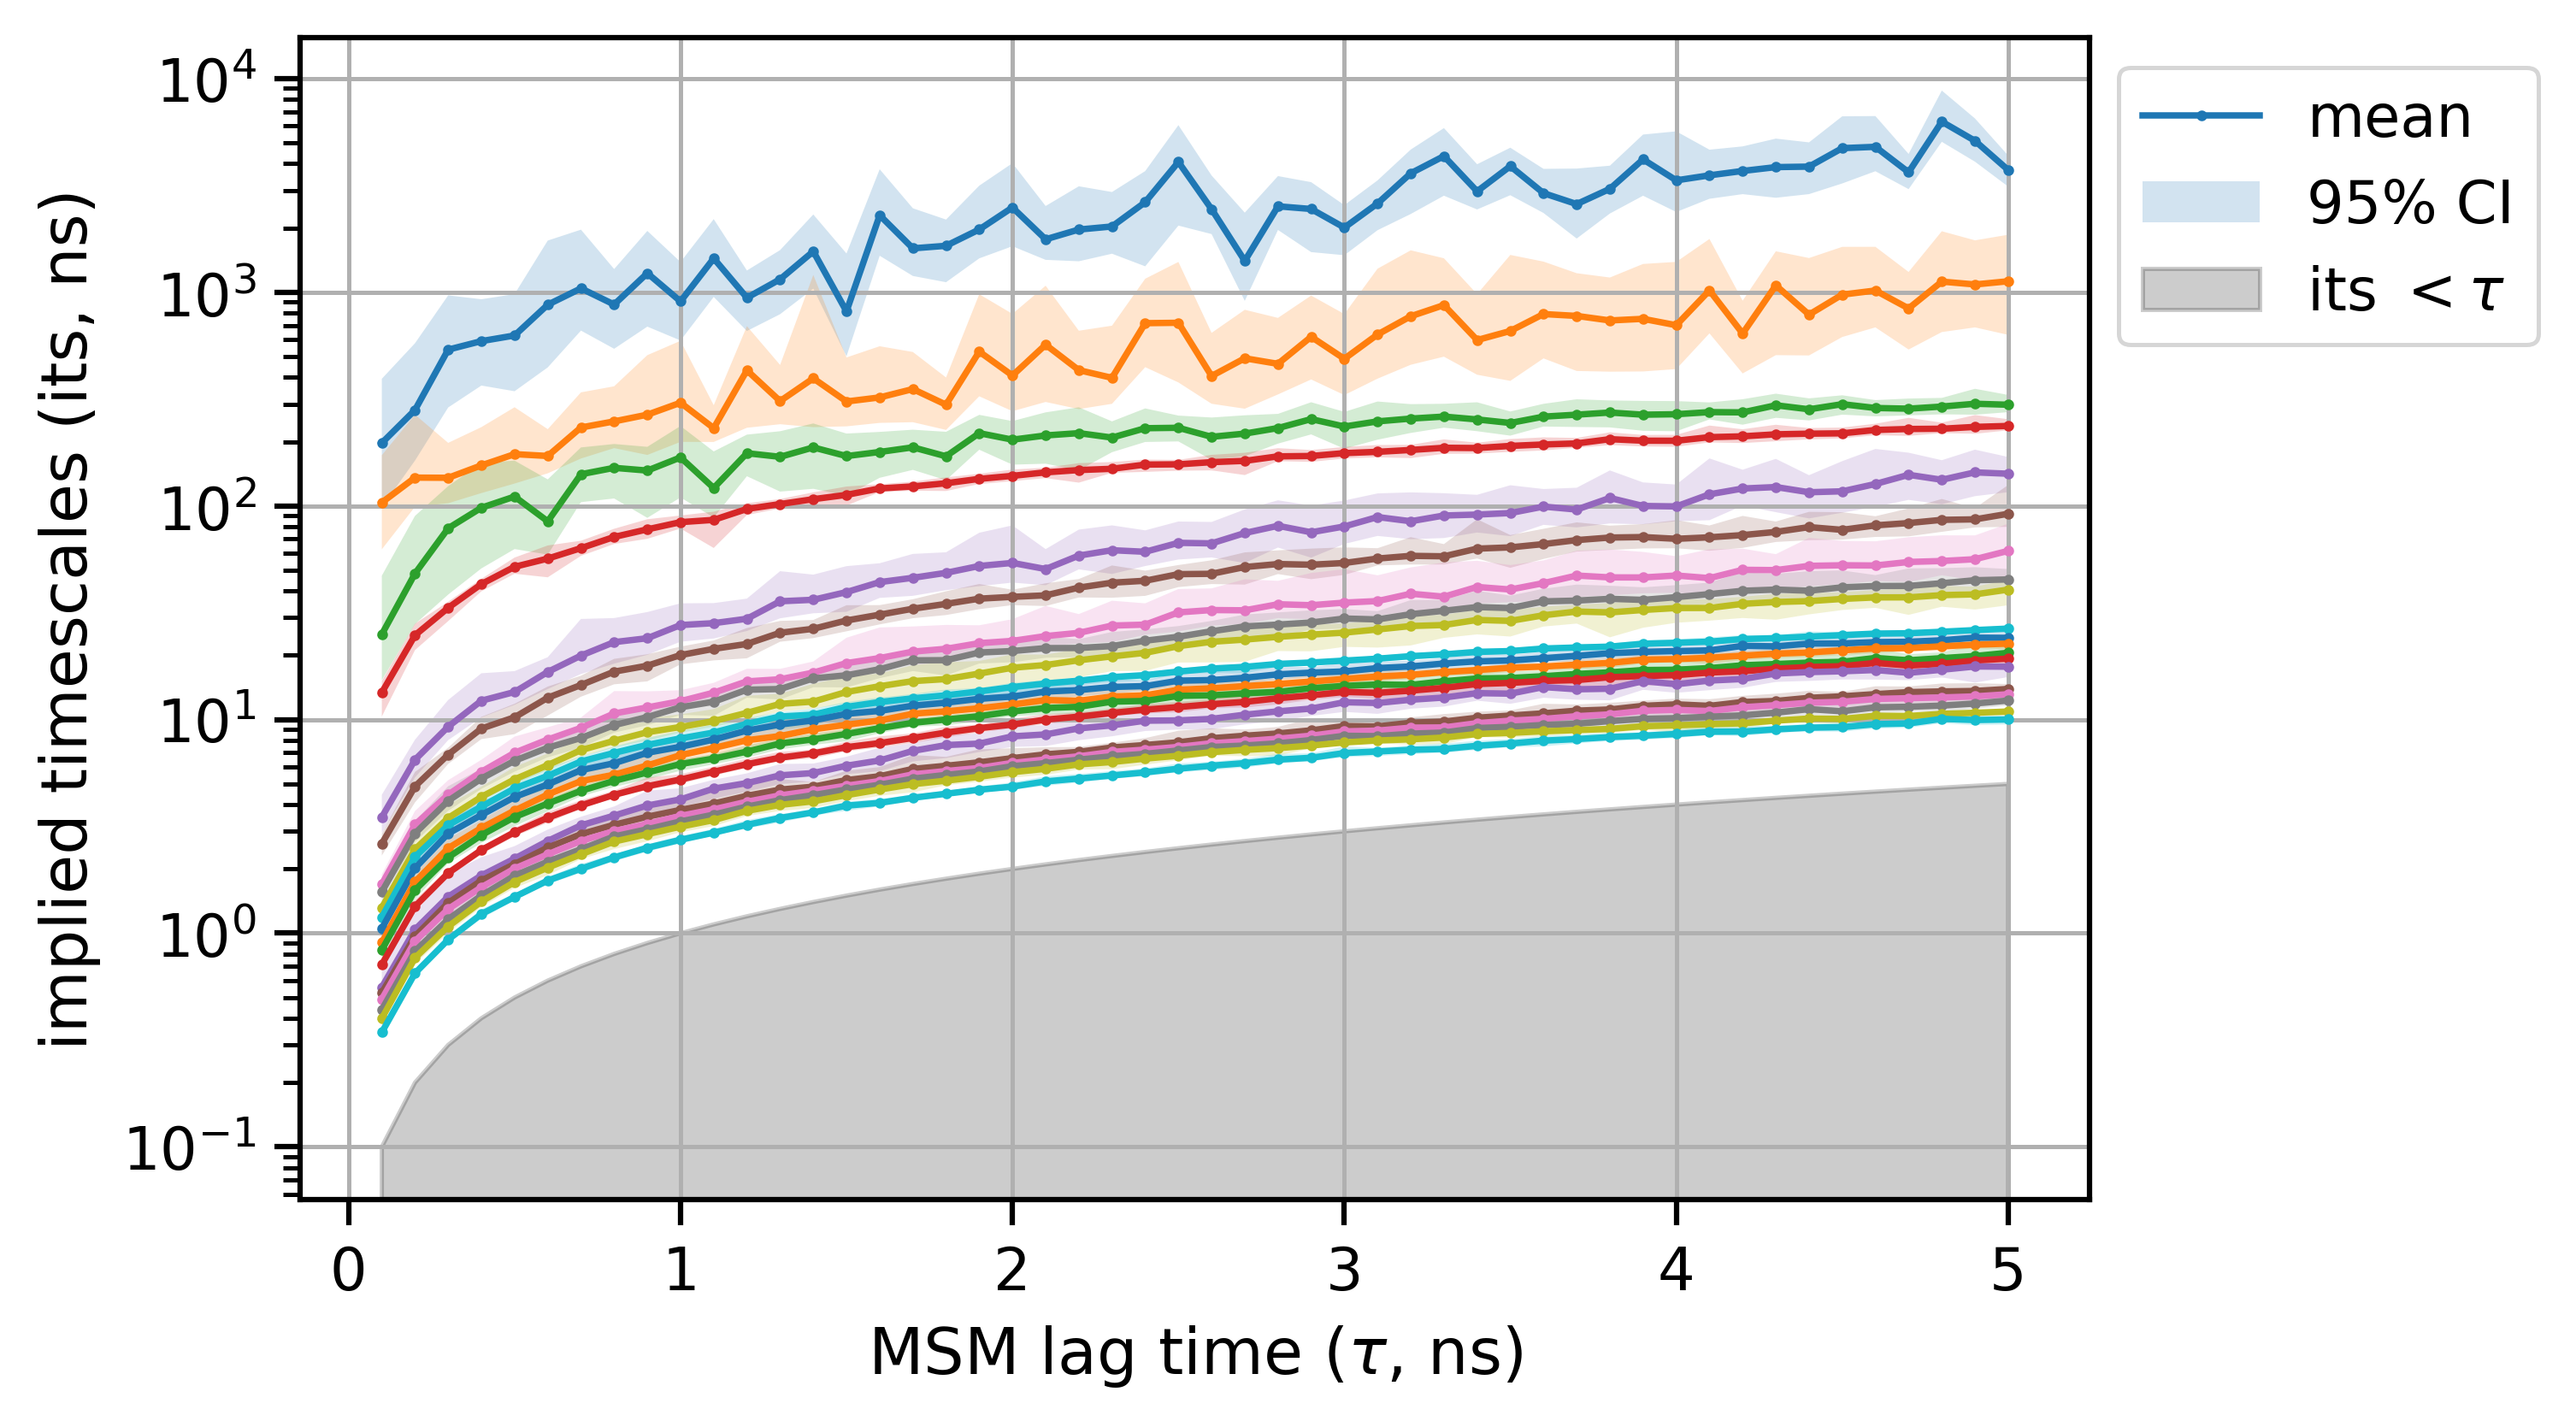
\includegraphics[width=0.4\linewidth]{chapters/msm_optimization/figures/aadh_implied_timescales_short.png}}
    
    \subtop[$1<\tau^{MSM}<\SI{50}{\nano\second}$\label{fig:aadh_its_long}]{
        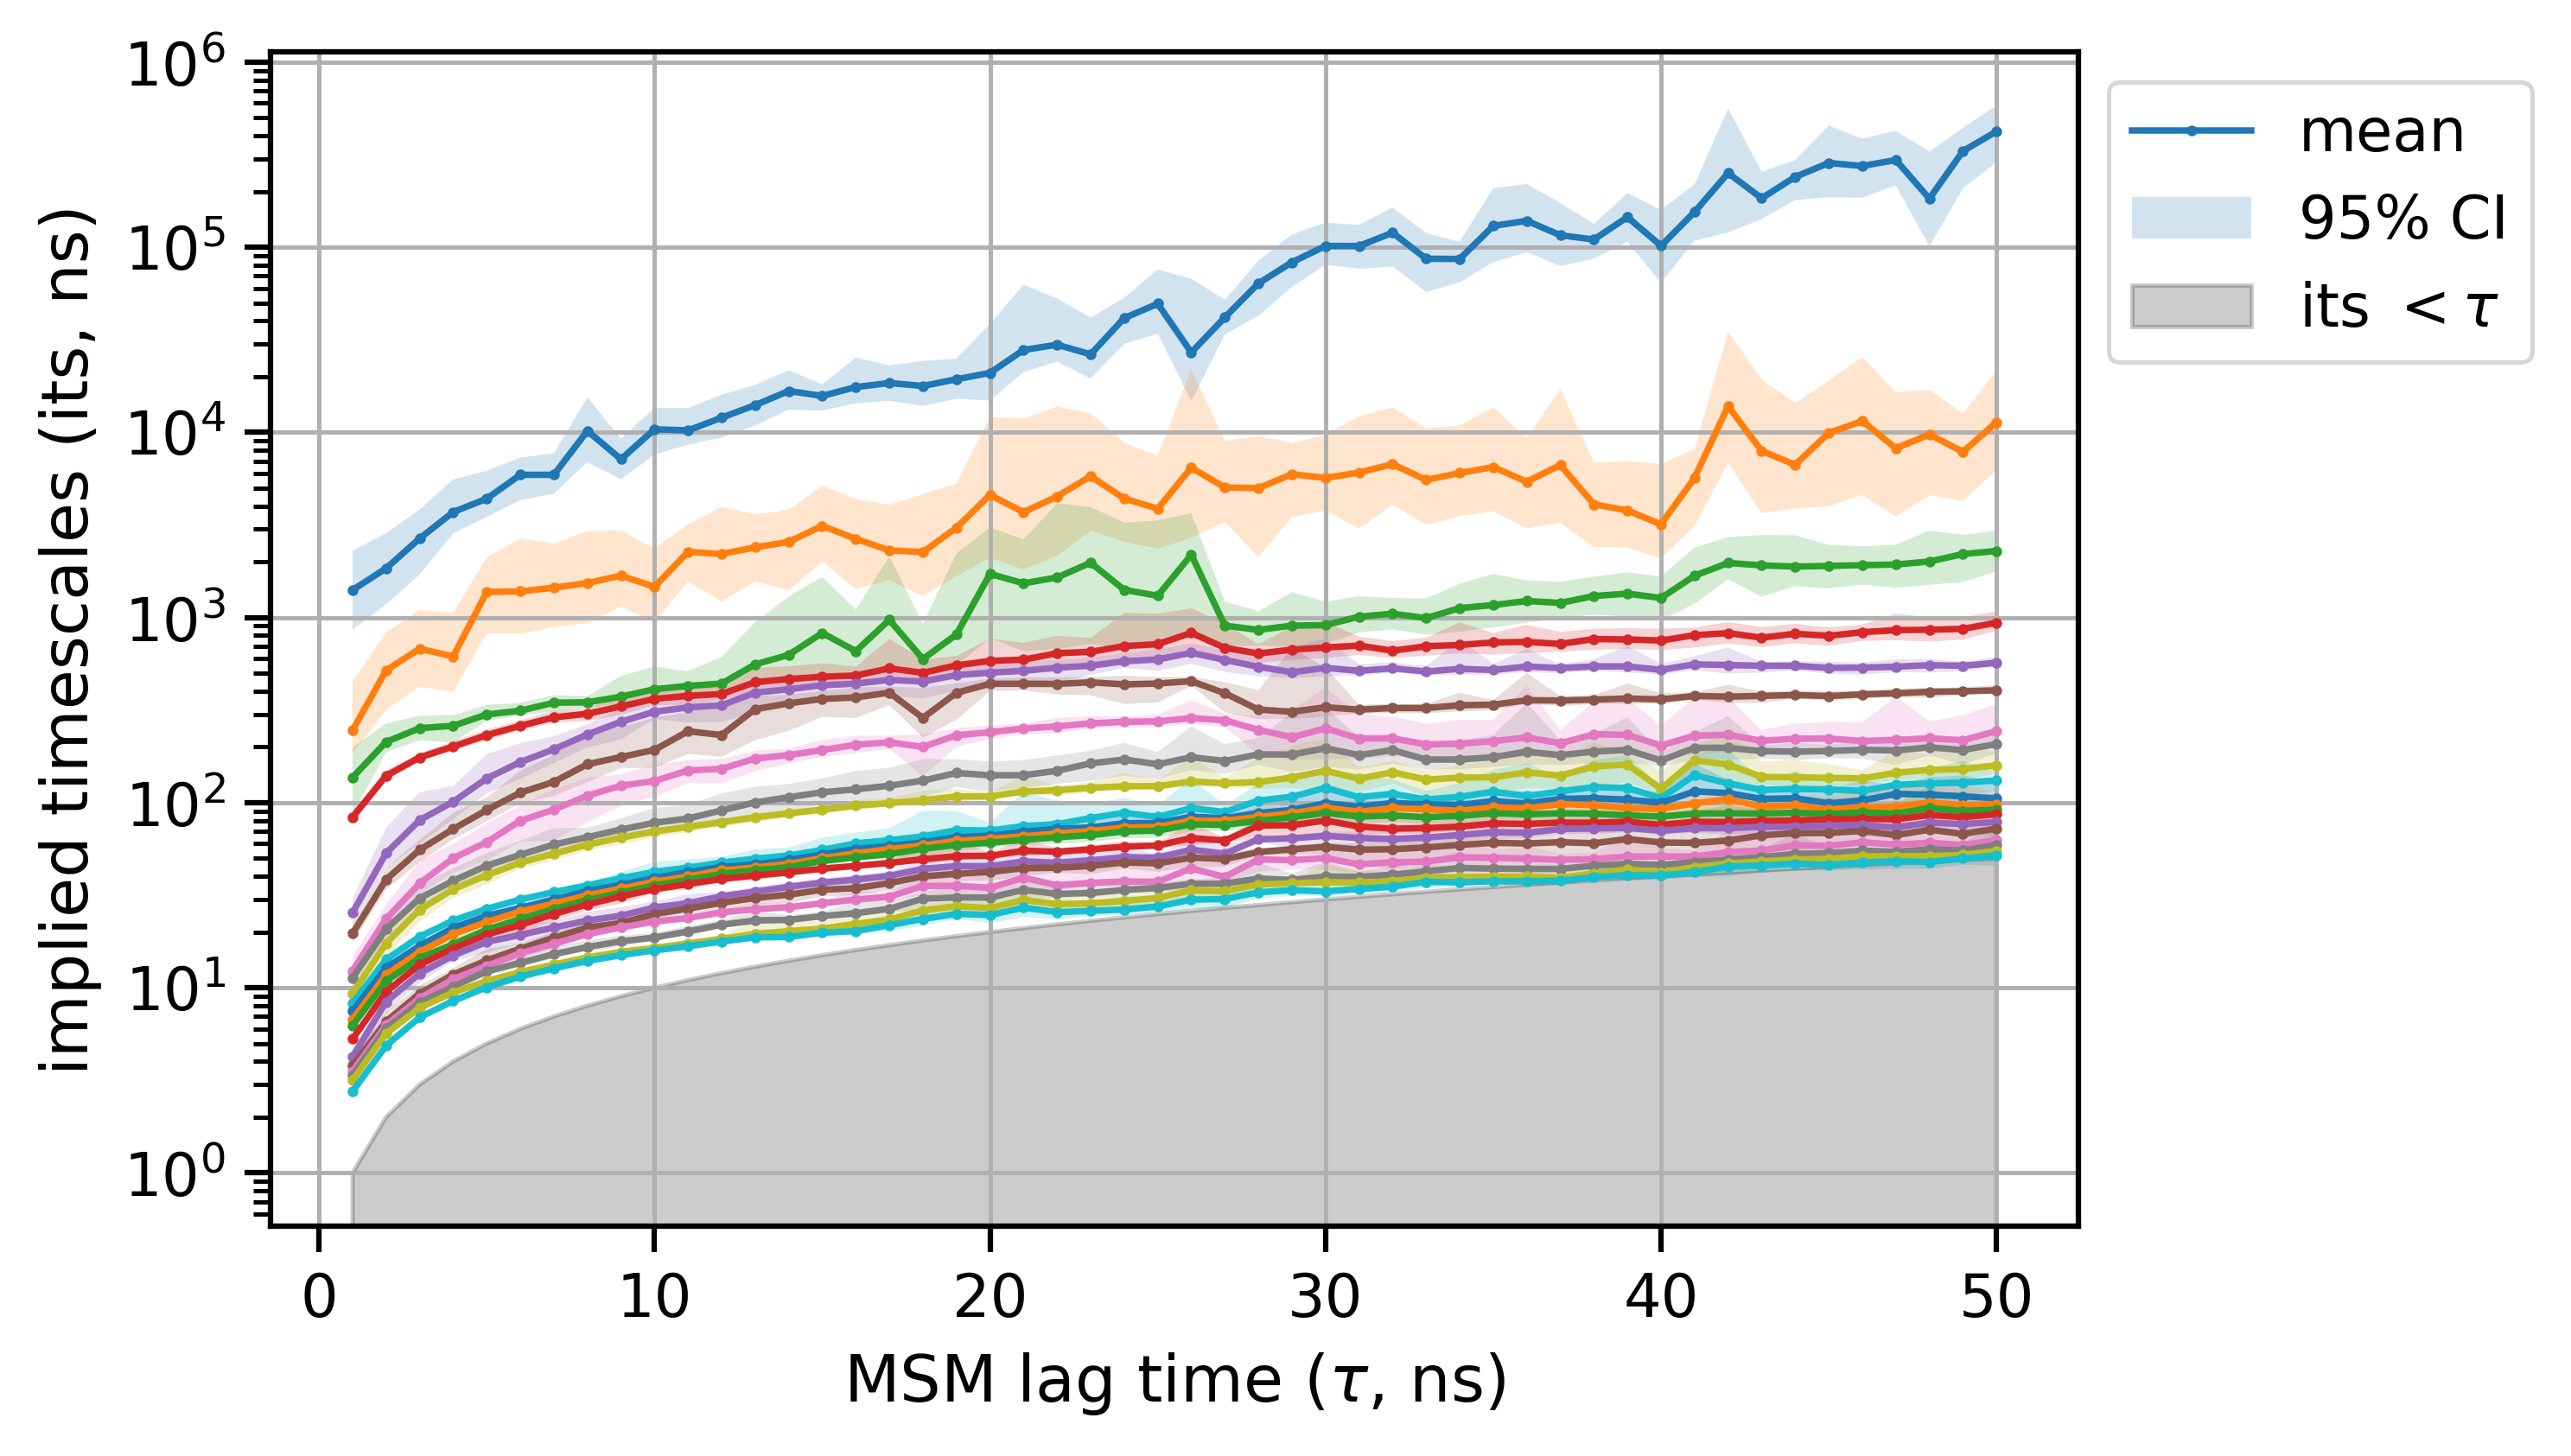
\includegraphics[width=0.4\linewidth]{chapters/msm_optimization/figures/aadh_implied_timescales_long.png}}
\end{figure}


\begin{figure}[ht!]
    \centering
    \caption{Optimised response surface}
    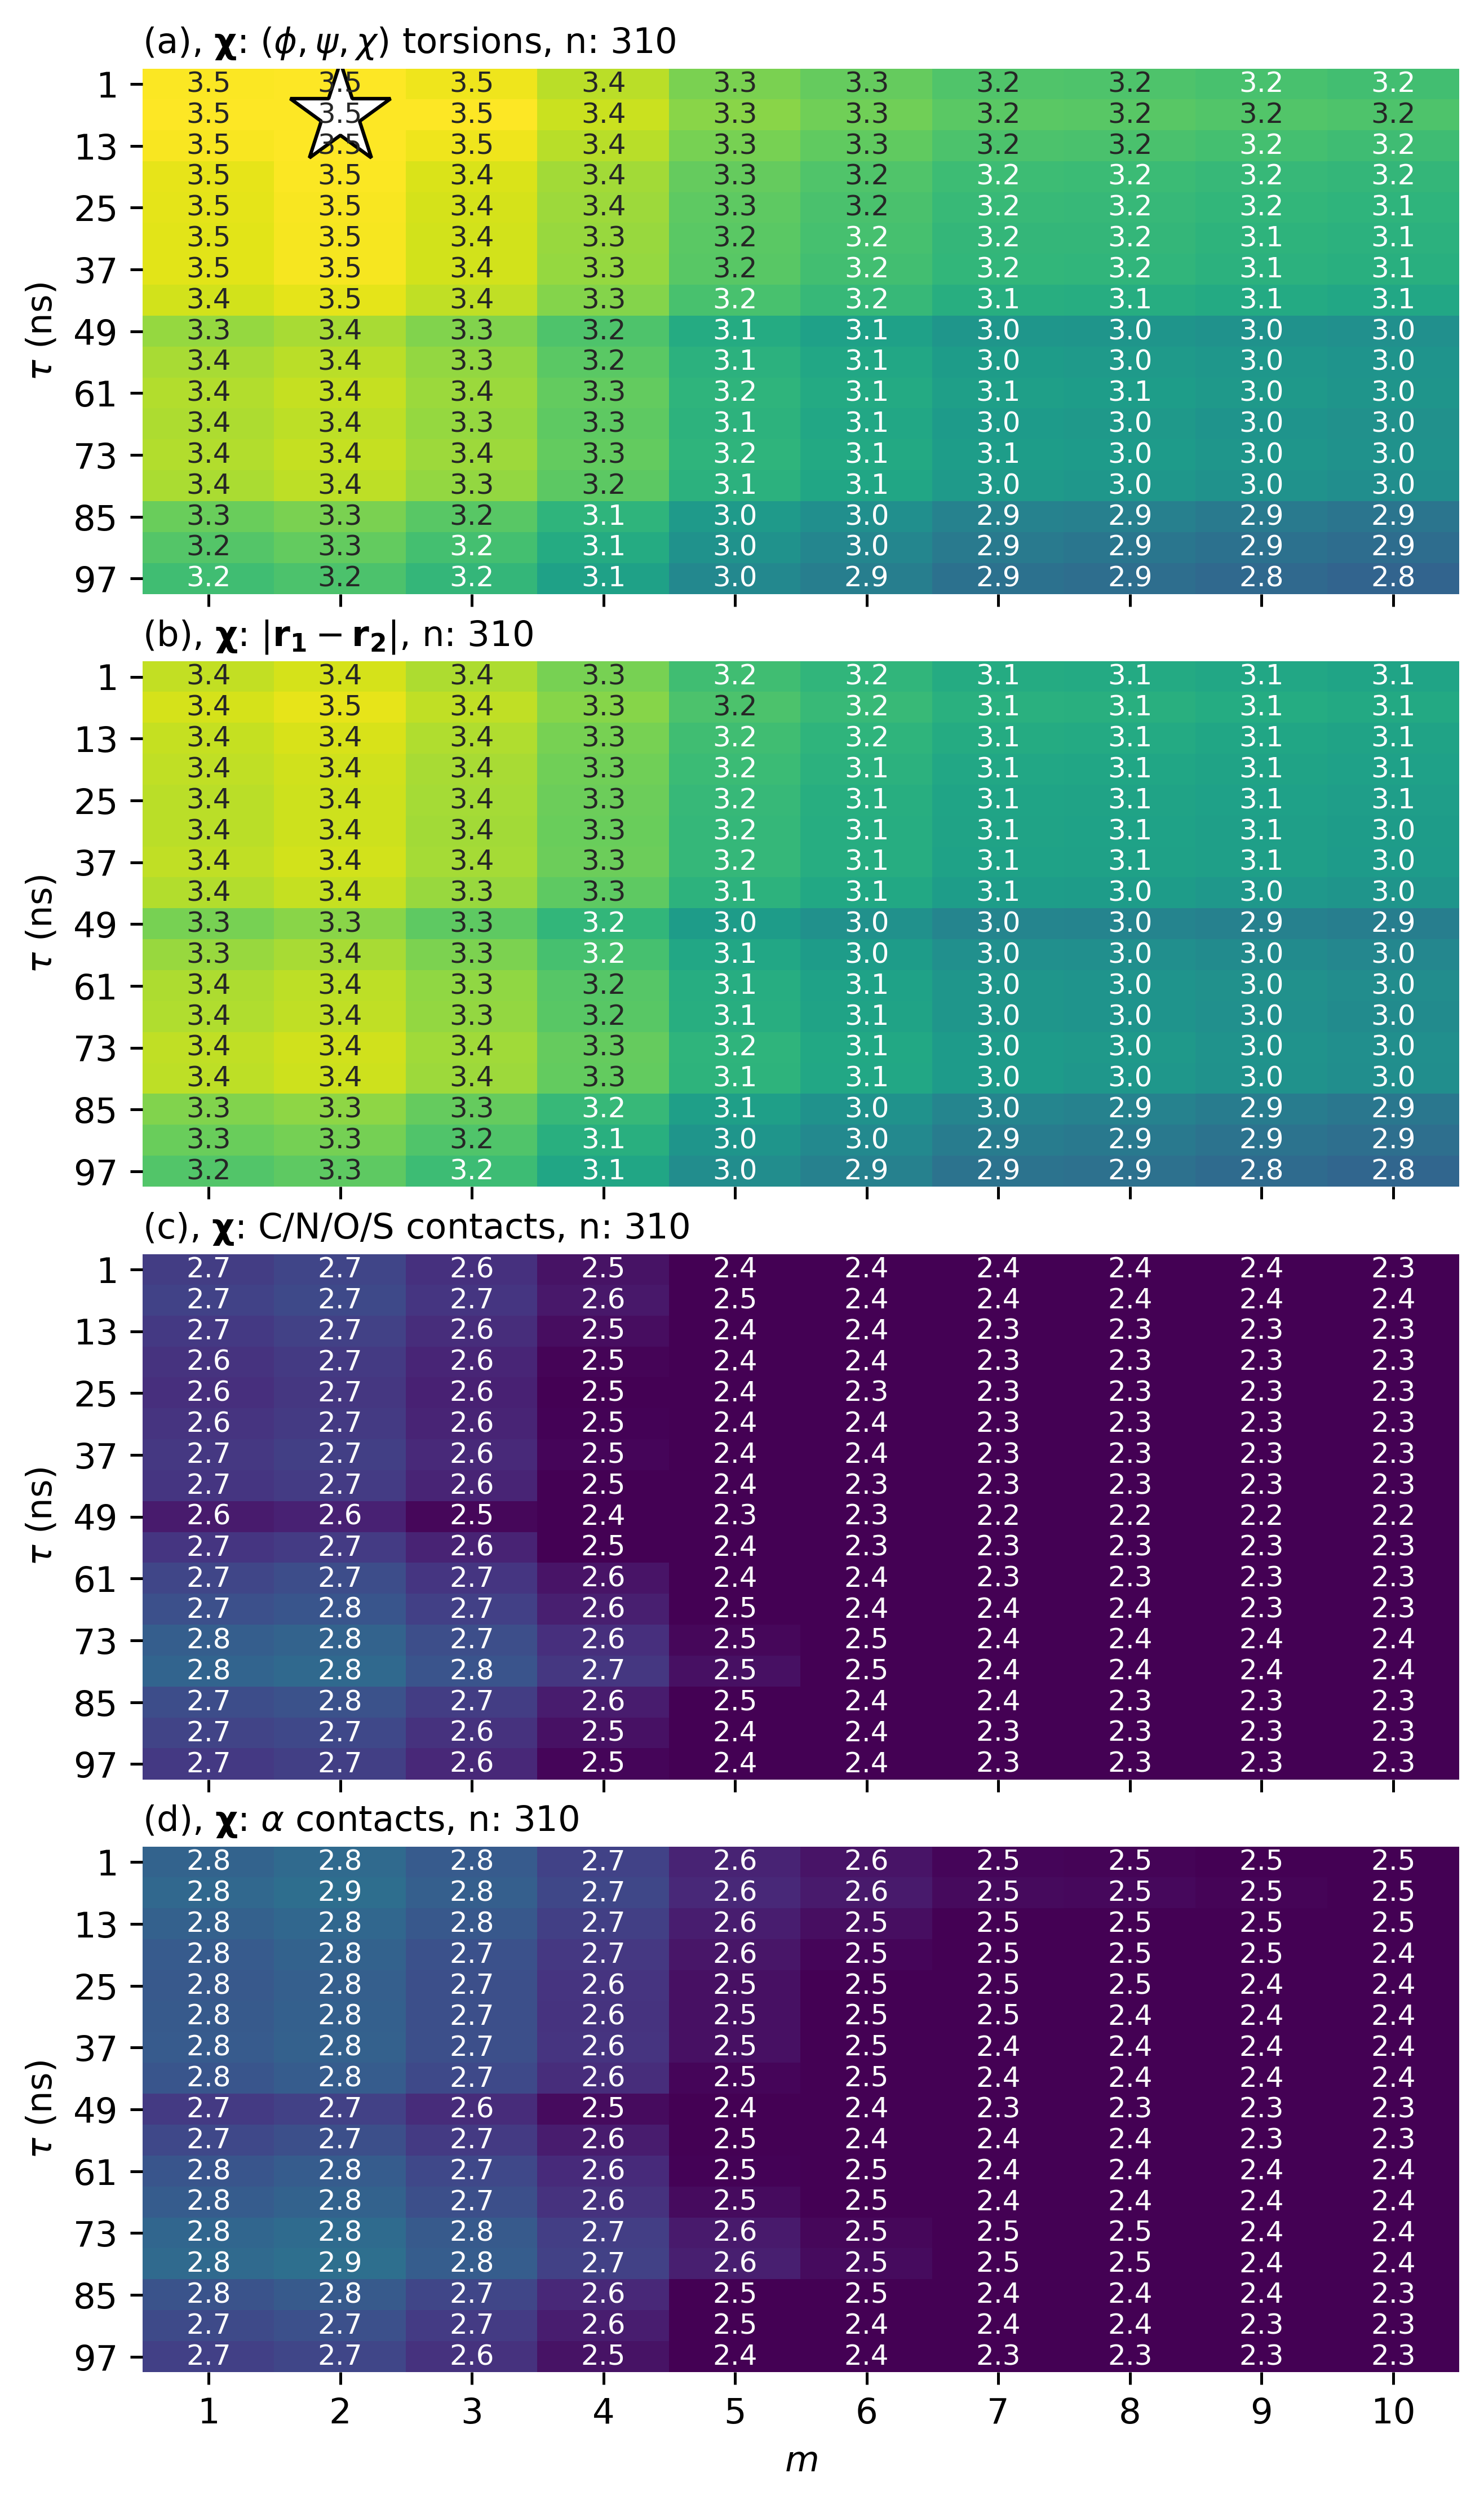
\includegraphics[width=0.8\textwidth]{chapters/msm_optimization/figures/aadh_response_surface_d_opt.png.png}
    \label{fig:aadh_rsm_opt}
\end{figure}



So far the response surface for AADH has been modelled and optimised with a combination of randomly sampling and Bayesian optimisation under two assumptions about the model specification: that $\tau^{MSM}$ and $k$, the number of eigenvalues in the VAMP-2 score, are correctly specified. To test this figure \ref{fig:aadh_its} shows the eigenvalue spectrum as a function of $\tau^{MSM}$ for the optimum hyperparameters. Panel (a) shows detail around the  $\tau^{MSM} \simeq 2$ which clearly shows the top three implied timescales \footnote{$k=4$ in the VAMP-2 score but this includes the trivial eigenvalue $\lambda = 1$} are increasing albeit slowly which suggests that $\tau^{MSM}$ is too small. Looking at the implied timescales on a longer timescale $1 < \tau^{MSM} < \SI{50}{\nano\second}$ (panel (b)) shows that the longest relaxation process never becomes independent of $\tau$, while the second longest process does become independent at around $\SI{20}{ns}$. 

At $\tau = \SI{2}{\nano\second}$ there is a clear separation of timescales between the fourth and and fifth timescales suggesting $k=5$ would be more appropriate. However at $\tau = \SI{20}{\nano\second}$ a there is a clear separation between the third and fourth timescale, suggesting the value used in the original specification, $k=4$, is appropriate.  The question of how many metastable states, corresponding to how many time scales can be considered dominant, will be investigated in chapter \ref{chap:hmm}. 

It is not clear whether changing the value of $\tau^{MSM}$ or $k$ in the VAMP-2 definition will change the optimum hyper-parameters. If the character of relaxation processes doesn't change then differences in $\tau^{MSM}$ are unlikely to change the optimum hyper-parameters, although the absolute values of the response surface will change. Given the discontinuity in the second relaxation process at $\SI{6}{\nano\second}$ this may not be apply here. Including additional fast relaxation processes, as has occurred here, in the definition of the response is again unlikely to affect the optimum, however the obverse is unlikely to be true.

Despite these limitations, knowledge of the response surface and of the eigenvalue spectrum suggests sensitivity analyses and further work to understand the validity of the MSM.  The goal of sensitivity analyses is to have faith that reasonable changes in model choices and hyper-parameters do not materially affect inferences from the model. Typically we are concerned with inferring relaxation timescales ($t_{i}$), the character of the relaxation process ($\Psi_{i}$) and the lumping of the microstates into metastable states. The VAMP-2 score has served as a proxy for the inferences required from the model but this is not sufficient  for a number of reasons.  First, as discussed above it will be sensitive to both the MSM lag time and the number of eigenfunctions used in the definition. Second, as figure \ref{fig:ala1_evcompare} has demonstrated, VAMP-2 is not sensitive to the discretisation error. Third, the phenomenon of the Rashomon effect \cite{BreimanStatisticalModeling} in statistical modelling, where  multiple \emph{different} statistical models result in the performance metric, could be at play here.

The standard validation check of MSMs, the Chapman-Kolmogorov test, relies on coarse graining transition matrix, which will be discussed in detail in chapter \ref{chap:hmm}. This discussion will center on the eigenvalue spectrum and qualitative aspects of the free energy surface and eigenfunctions.  For the optimal response surface, these are shown in figure \ref{fig:aadh_msm_best} and will serve as a base-case for the following sensitivity analyses informed by the response surface (figure \ref{fig:aadh_rsm_opt}) and eigenvalue spectrum (figure \ref{fig:aadh_its}).

\begin{figure}
    \centering
    \caption{MSM of AADH with optimum hyper-parameters: $\chi= (\phi, \psi, \chi)$ torsions, $\tau=\SI{10}{\nano\second}$, $m=2$ and $n=310$. Panels (a), (b) and (c) show the non-trivial eigenvectors used in the VAMP-2 score, the horizontal and vertical axes are the first two TICA components. Panel (d) are the first ten implied timescales, colored according to whether they were used in the VAMP-2 score. The error bars are the $\SI{95}{\percent}$ credible intervals.  Panel (e) is the free energy with the same axes as panels (a) - (c). The MSM was estimated using MCMC with 500 samples of the posterior.}
    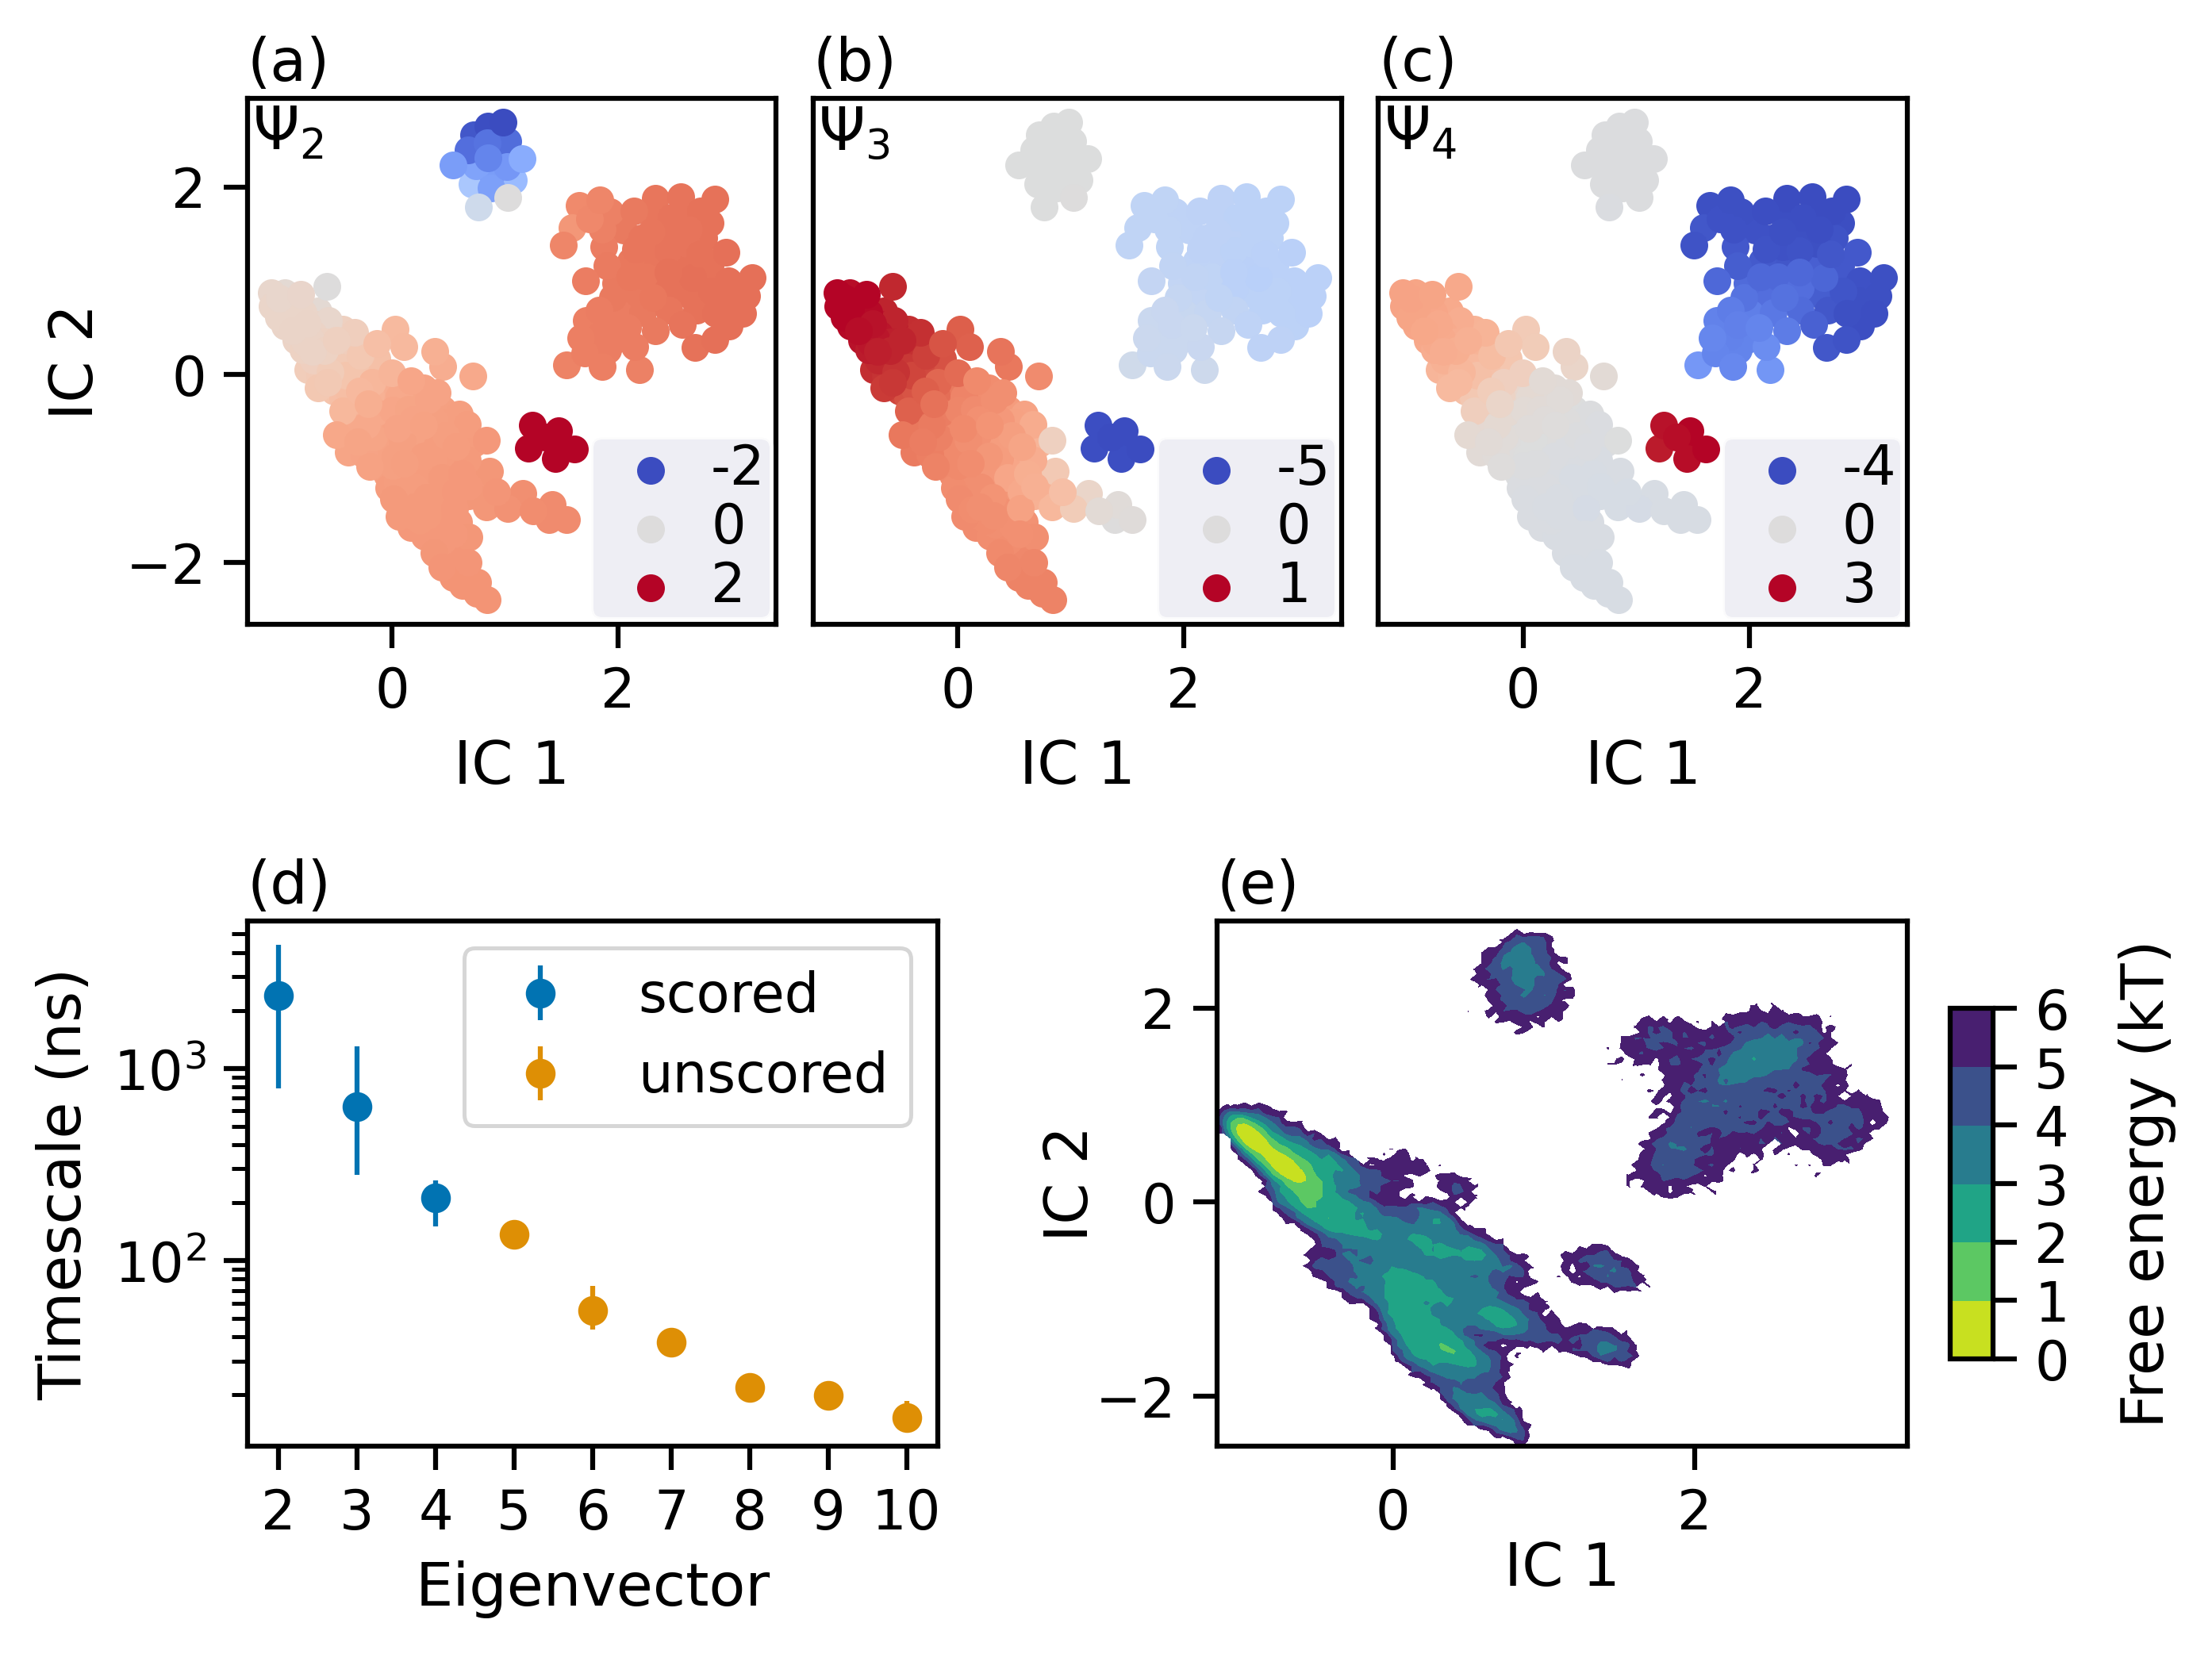
\includegraphics[width=0.8\textwidth]{chapters/msm_optimization/figures/aadh_msm_best.png}
    \label{fig:aadh_msm_best}
\end{figure}

Sensitivity 1, changed the MSM lag from $\SI{2}{\nano\second}$ to $\SI{20}{\nano\second}$ (figure xxx). This changed both the absolute and relative values of the three slowest implied timescales. For example in the base case $t_2/t_4 \simeq 10$ where as in sensitivity 1, $t_2/t_4 \simeq 100$. However, the sign structure of both $\Psi_{2}$ and $\Psi_{3}$ did not change which suggest that the implied metastable states are unlikely to be affected.  

\begin{figure}
    \centering
    \caption{MSM of AADH, sensitivity 1}
    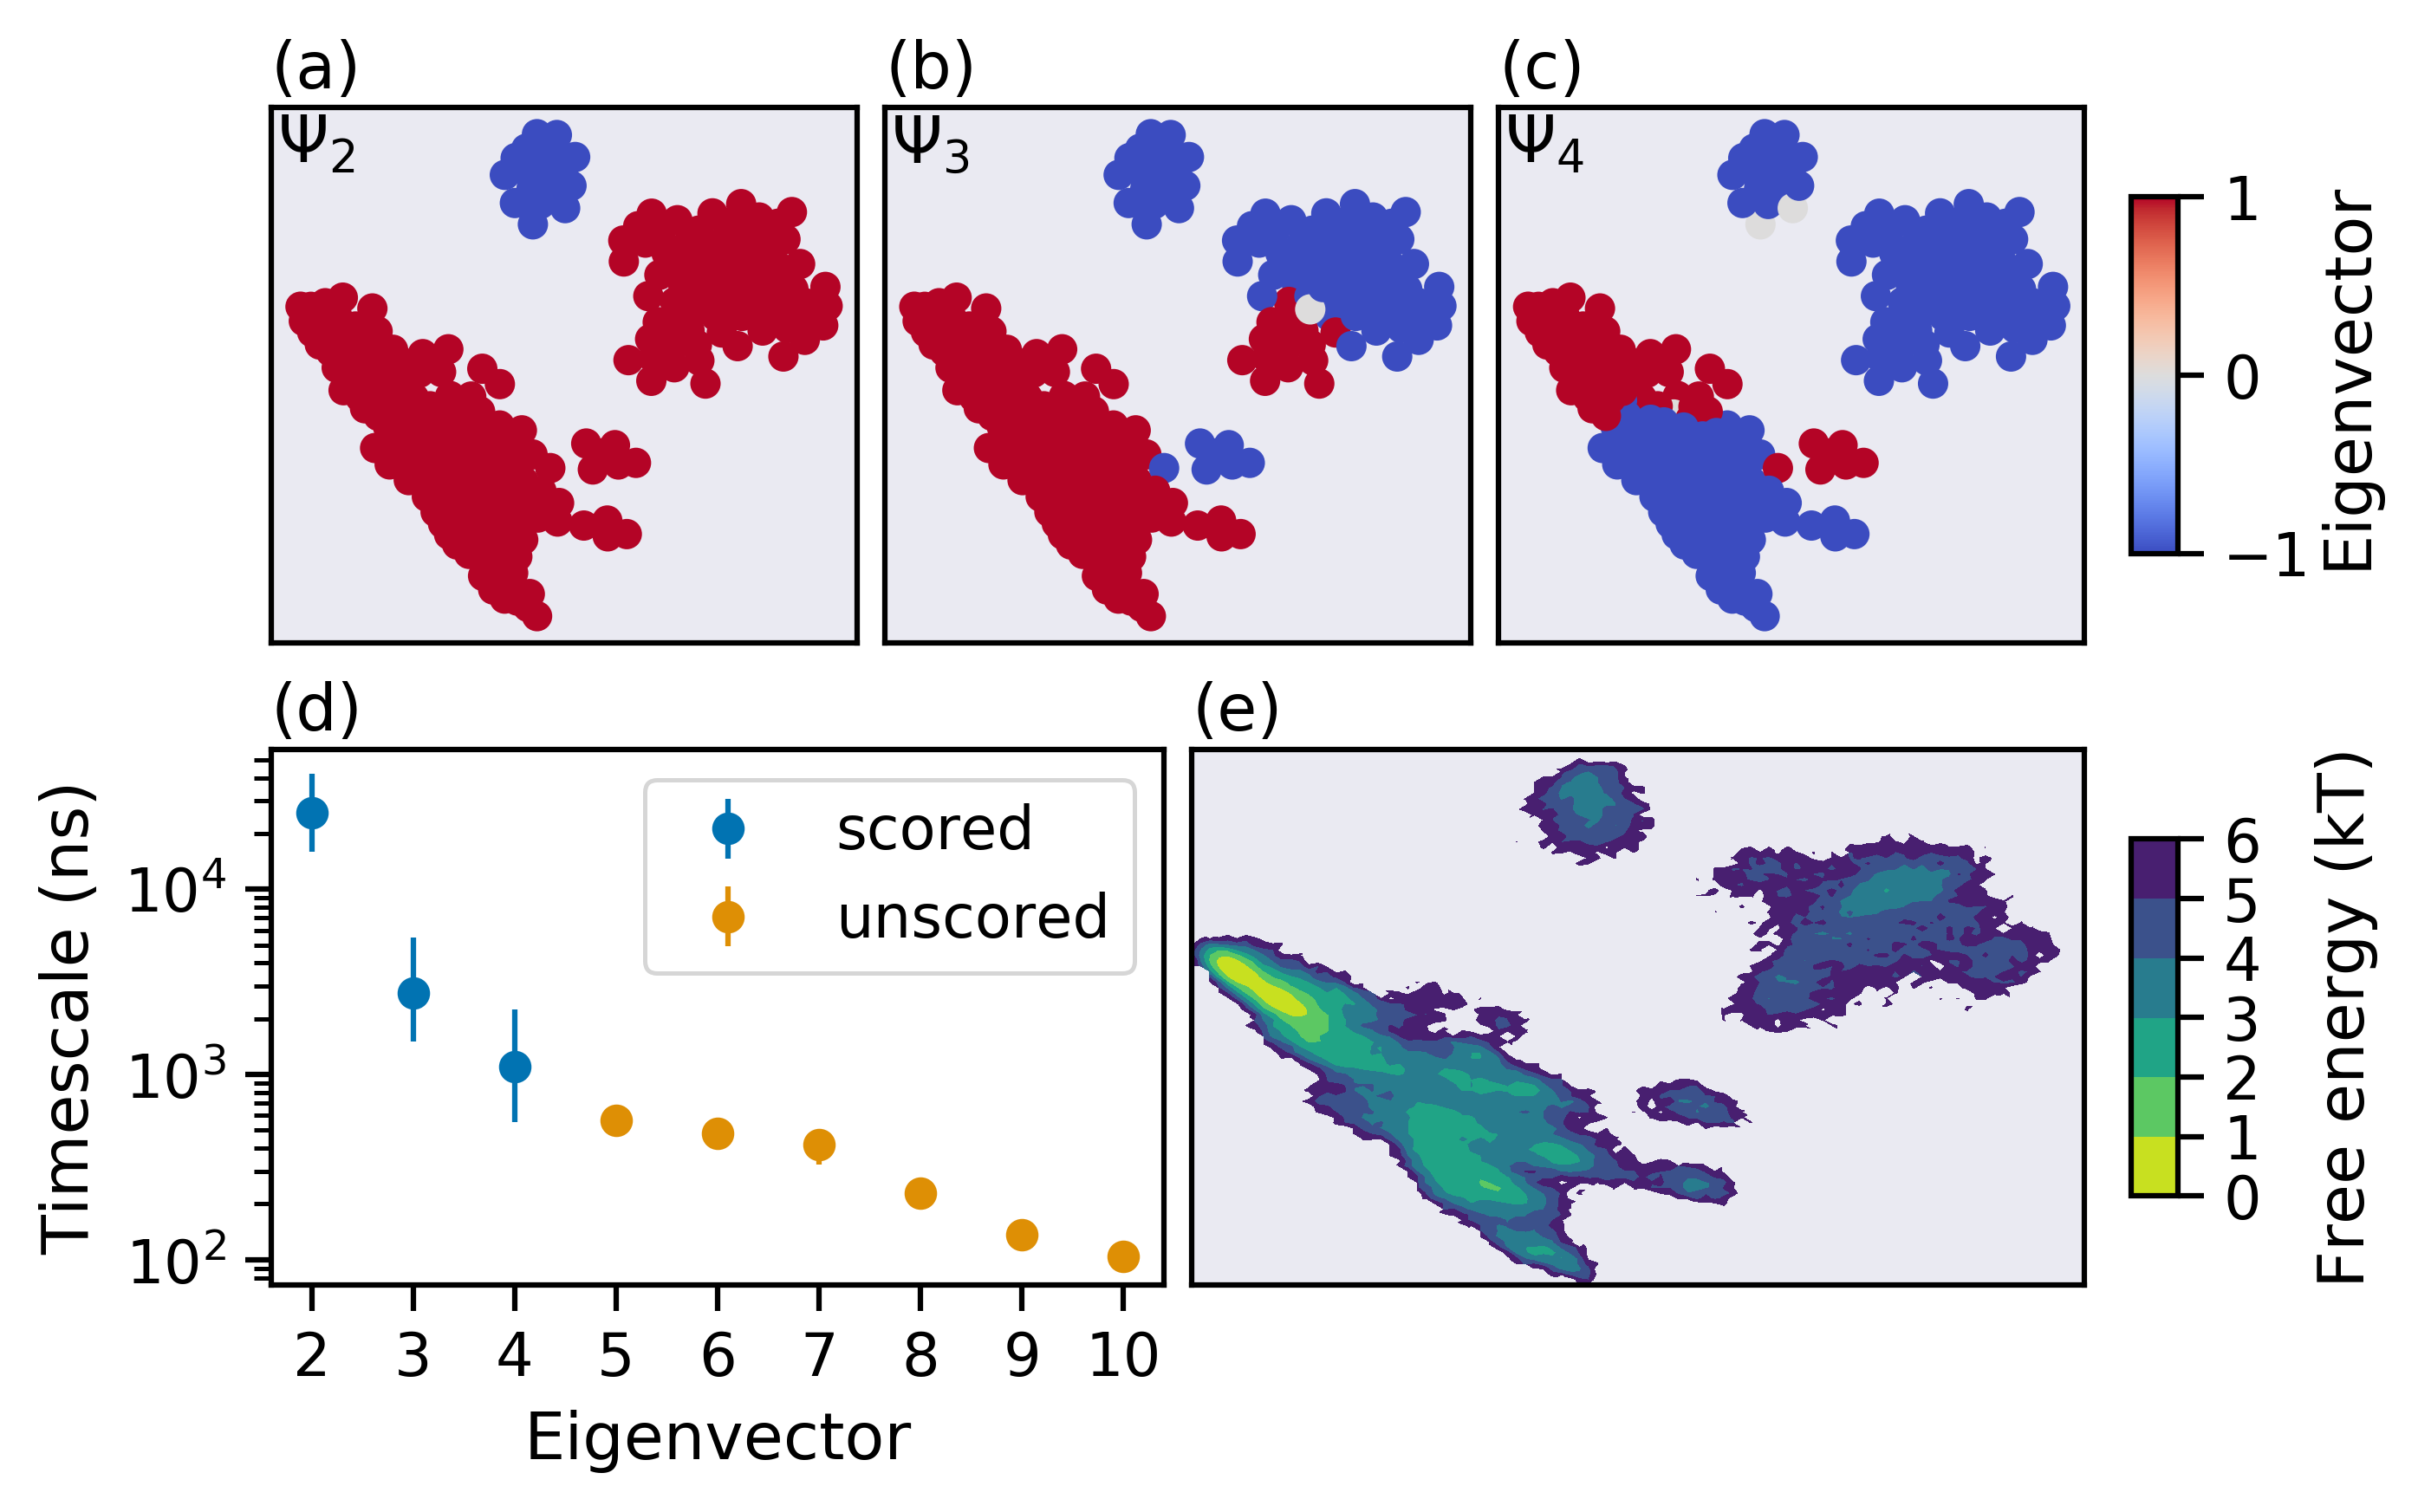
\includegraphics[width=0.8\textwidth]{chapters/msm_optimization/figures/aadh_msm_sens_1.png}
    \label{fig:aadh_msm_sens_1}
\end{figure}

Sensitivity 2, changed the hyper-parameters to the best performing set with the interatomic distances feature ($\tau = \SI{1}{\nano\second}, m=2, n=110$). This was justified because of the similarity in response values (incumbent: $\mu=3.56 \pm 0.18$, sensitivity 2: $\mu=3.44 \pm 0.35$). There is a clear similarity in the free energy surface and the sign structure of $\Psi_{2}$. There is a greater separation in timescales between $t_{2}$ and $t_{3}$ ($t_{2}/t_{3} \simeq 10$) than the base case ($t_{2}/t_{3} \simeq 3$) suggesting that $\Psi_{3}$ from the base case is not resolved by this feature. 
\begin{figure}
    \centering
    \caption{MSM of AADH, sensitivity 2}
    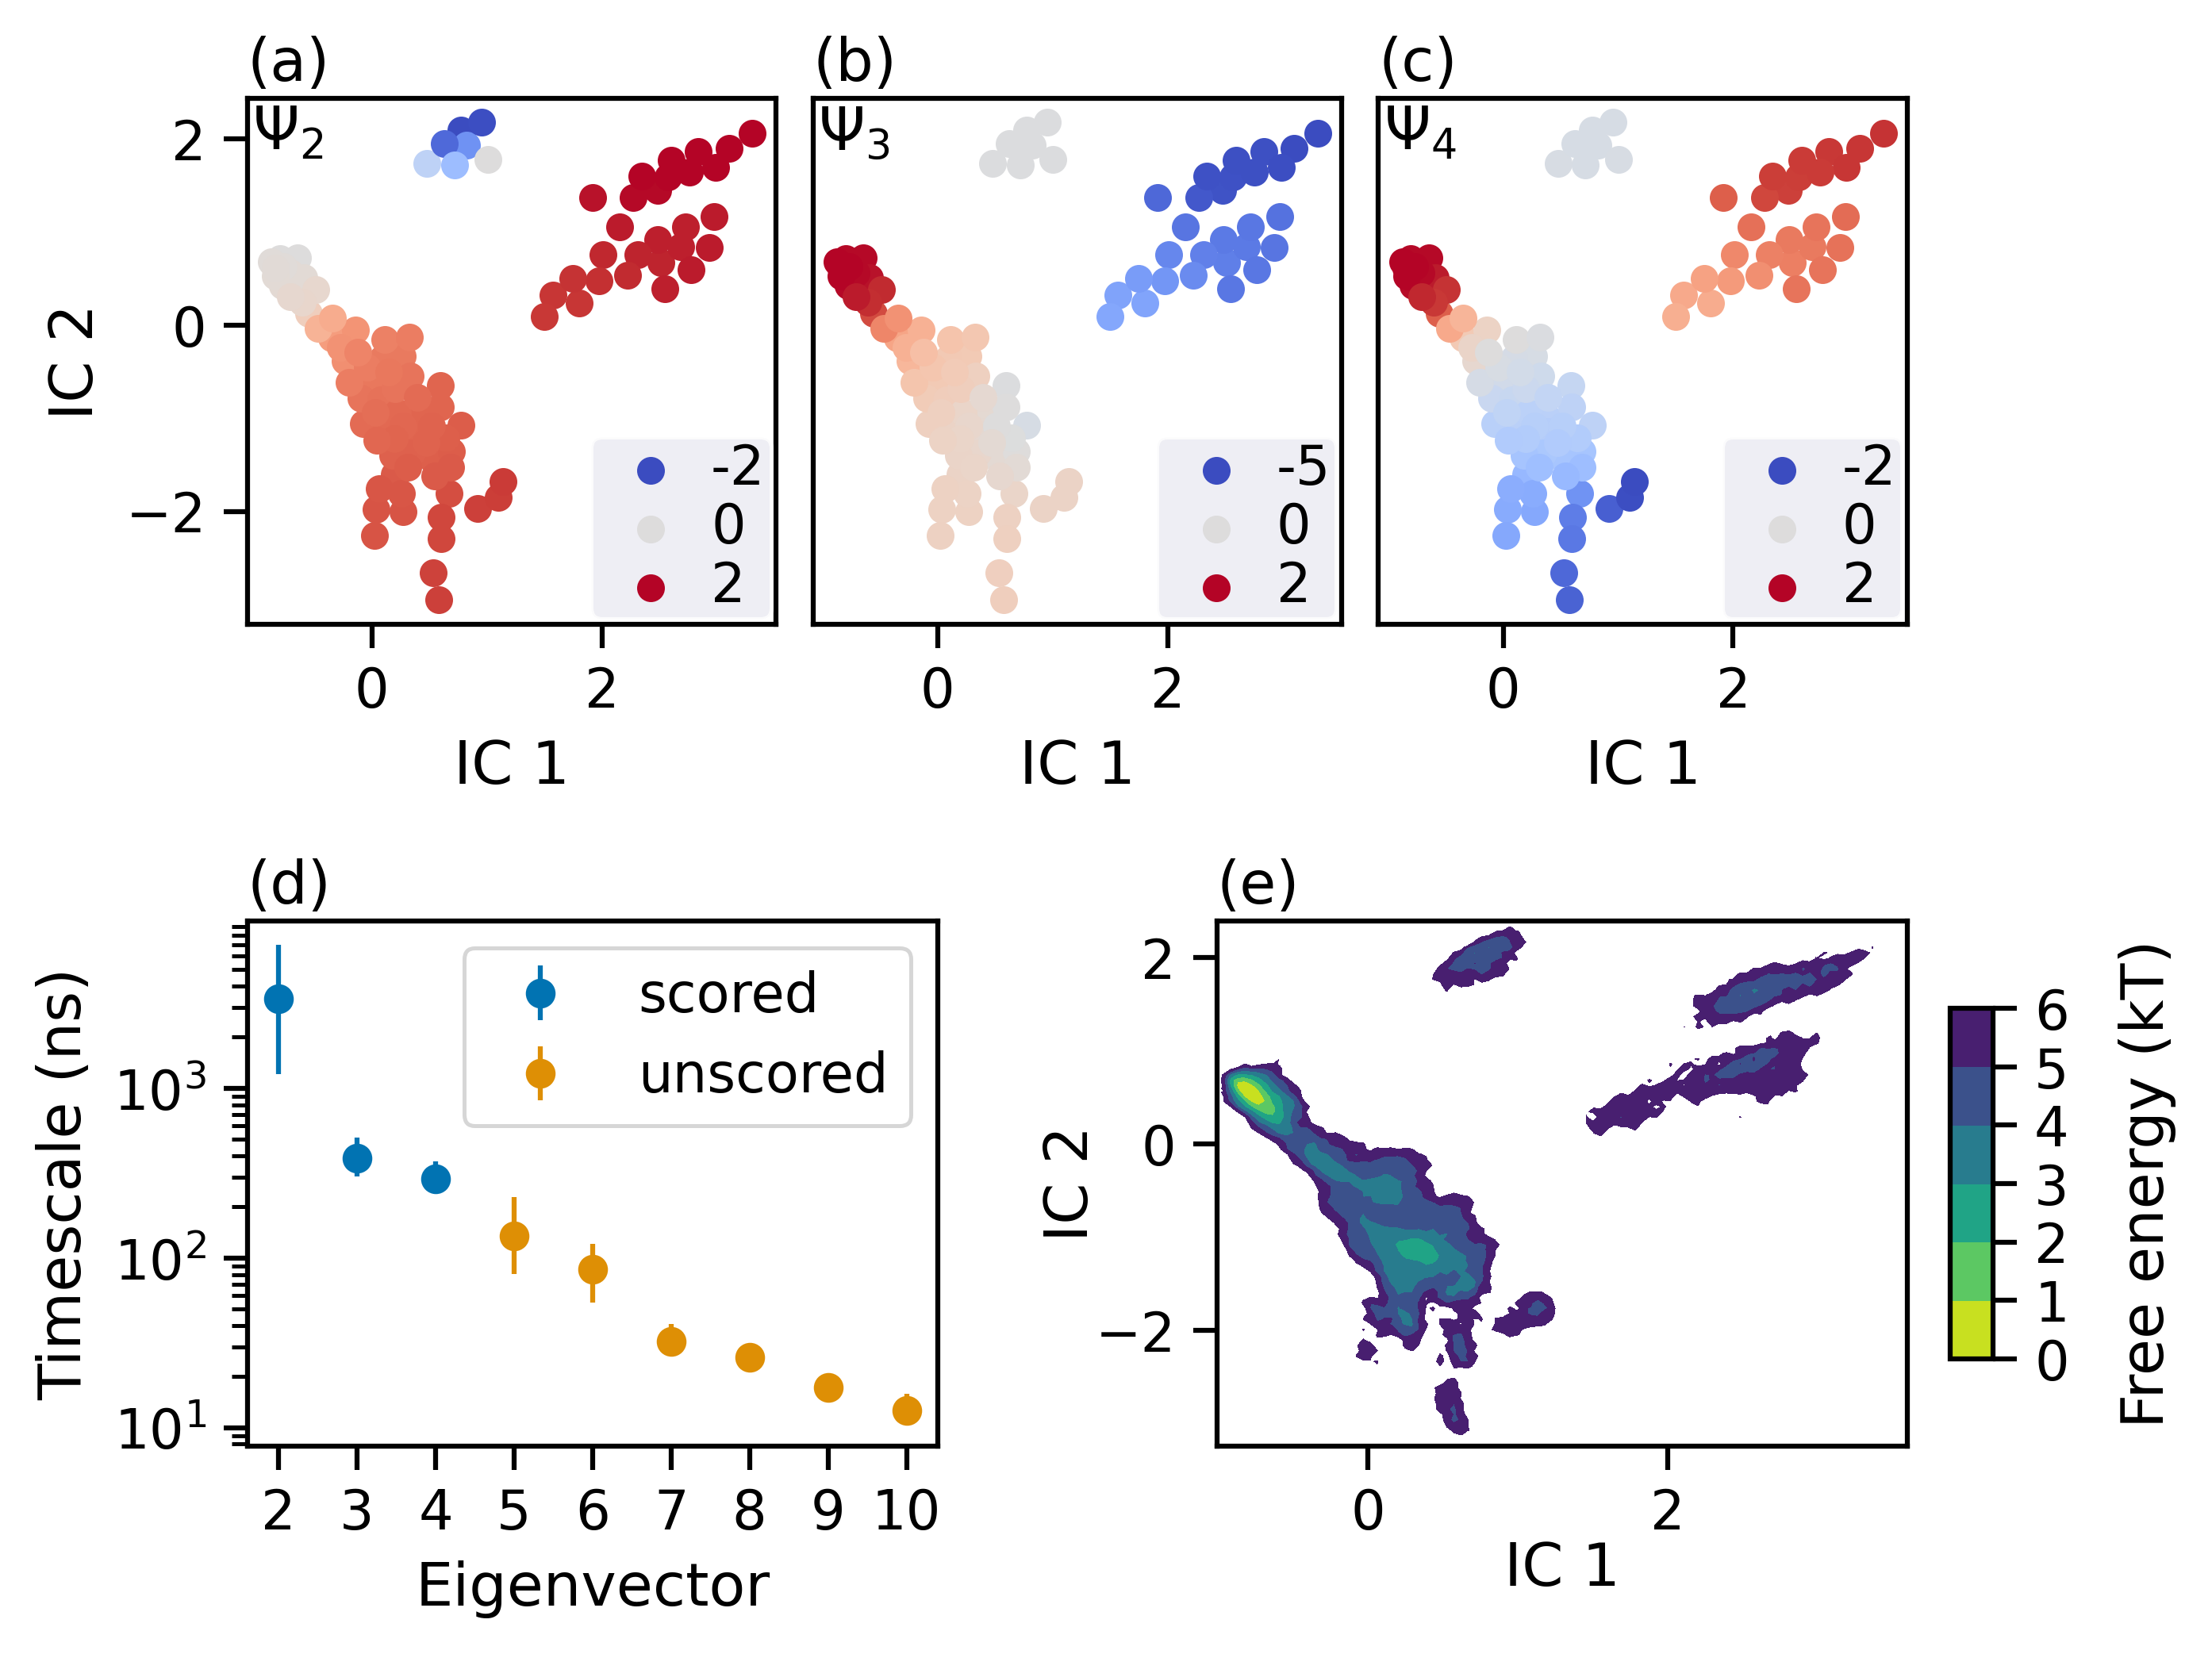
\includegraphics[width=0.8\textwidth]{chapters/msm_optimization/figures/aadh_msm_sens_2.png}
    \label{fig:aadh_msm_sens_2}
\end{figure}
Sensitivity 3, changed the value of $\tau$ to $\SI{85}{\nano\second}$ which is value of $\tau$ for which there is the smallest response values overlap with the incumbent (incumbent: $\mu=3.56 \pm 0.18$, sensitivity 3: $\mu=3.30 \pm 0.24$).  Here there is a distinct difference in the absolute values of the timescales and the free energy surface compared to the incumbent. The difference between the two TICA representations is significant: the normalized overlap between the two TICA components of the incumbent and sensitivity three is $0.63$ and $0.56$ and there are  differences in the weights attached to each feature shown in figure \ref{fig:aadh_msm_sens_3_tica}. 

\begin{figure}
    \centering
    \caption{MSM of AADH, sensitivity 3}
    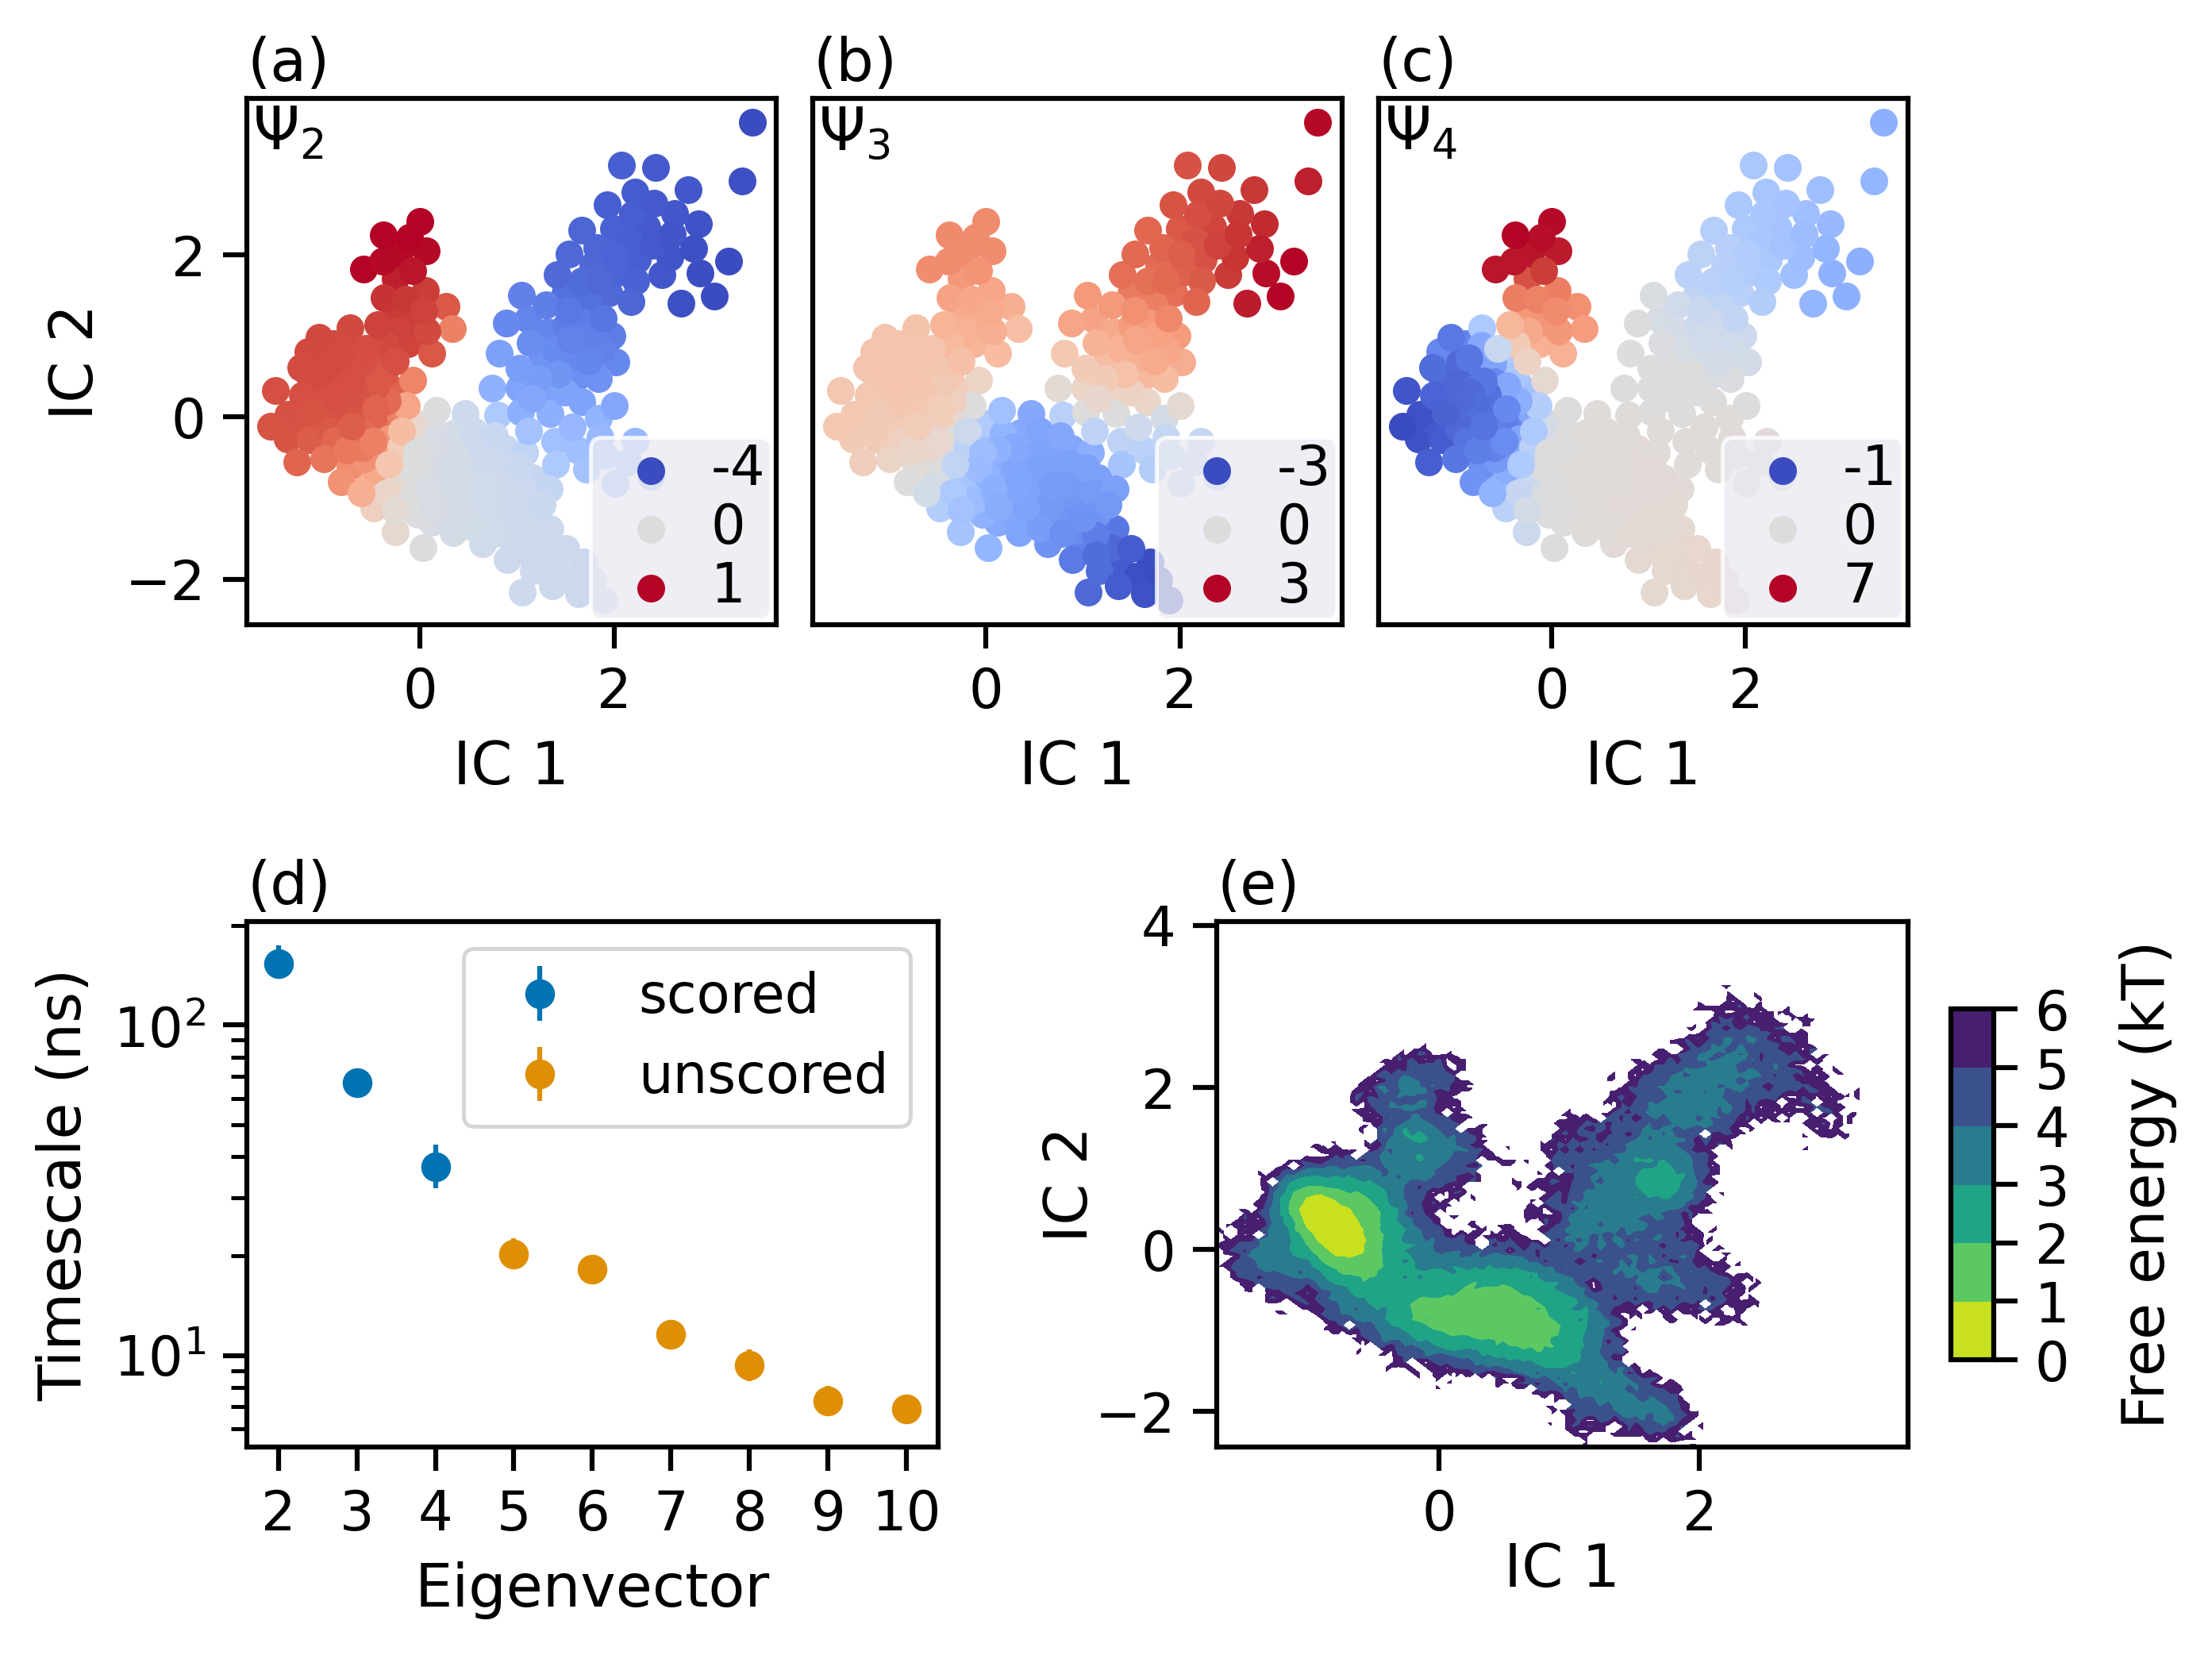
\includegraphics[width=0.8\textwidth]{chapters/msm_optimization/figures/aadh_msm_sens_3.png}
    \label{fig:aadh_msm_sens_3}
\end{figure}
\begin{figure}
    \centering
    \caption{Comparison of TICA eigenvectors between base case (blue) and sensitivity 3 (orange)}
    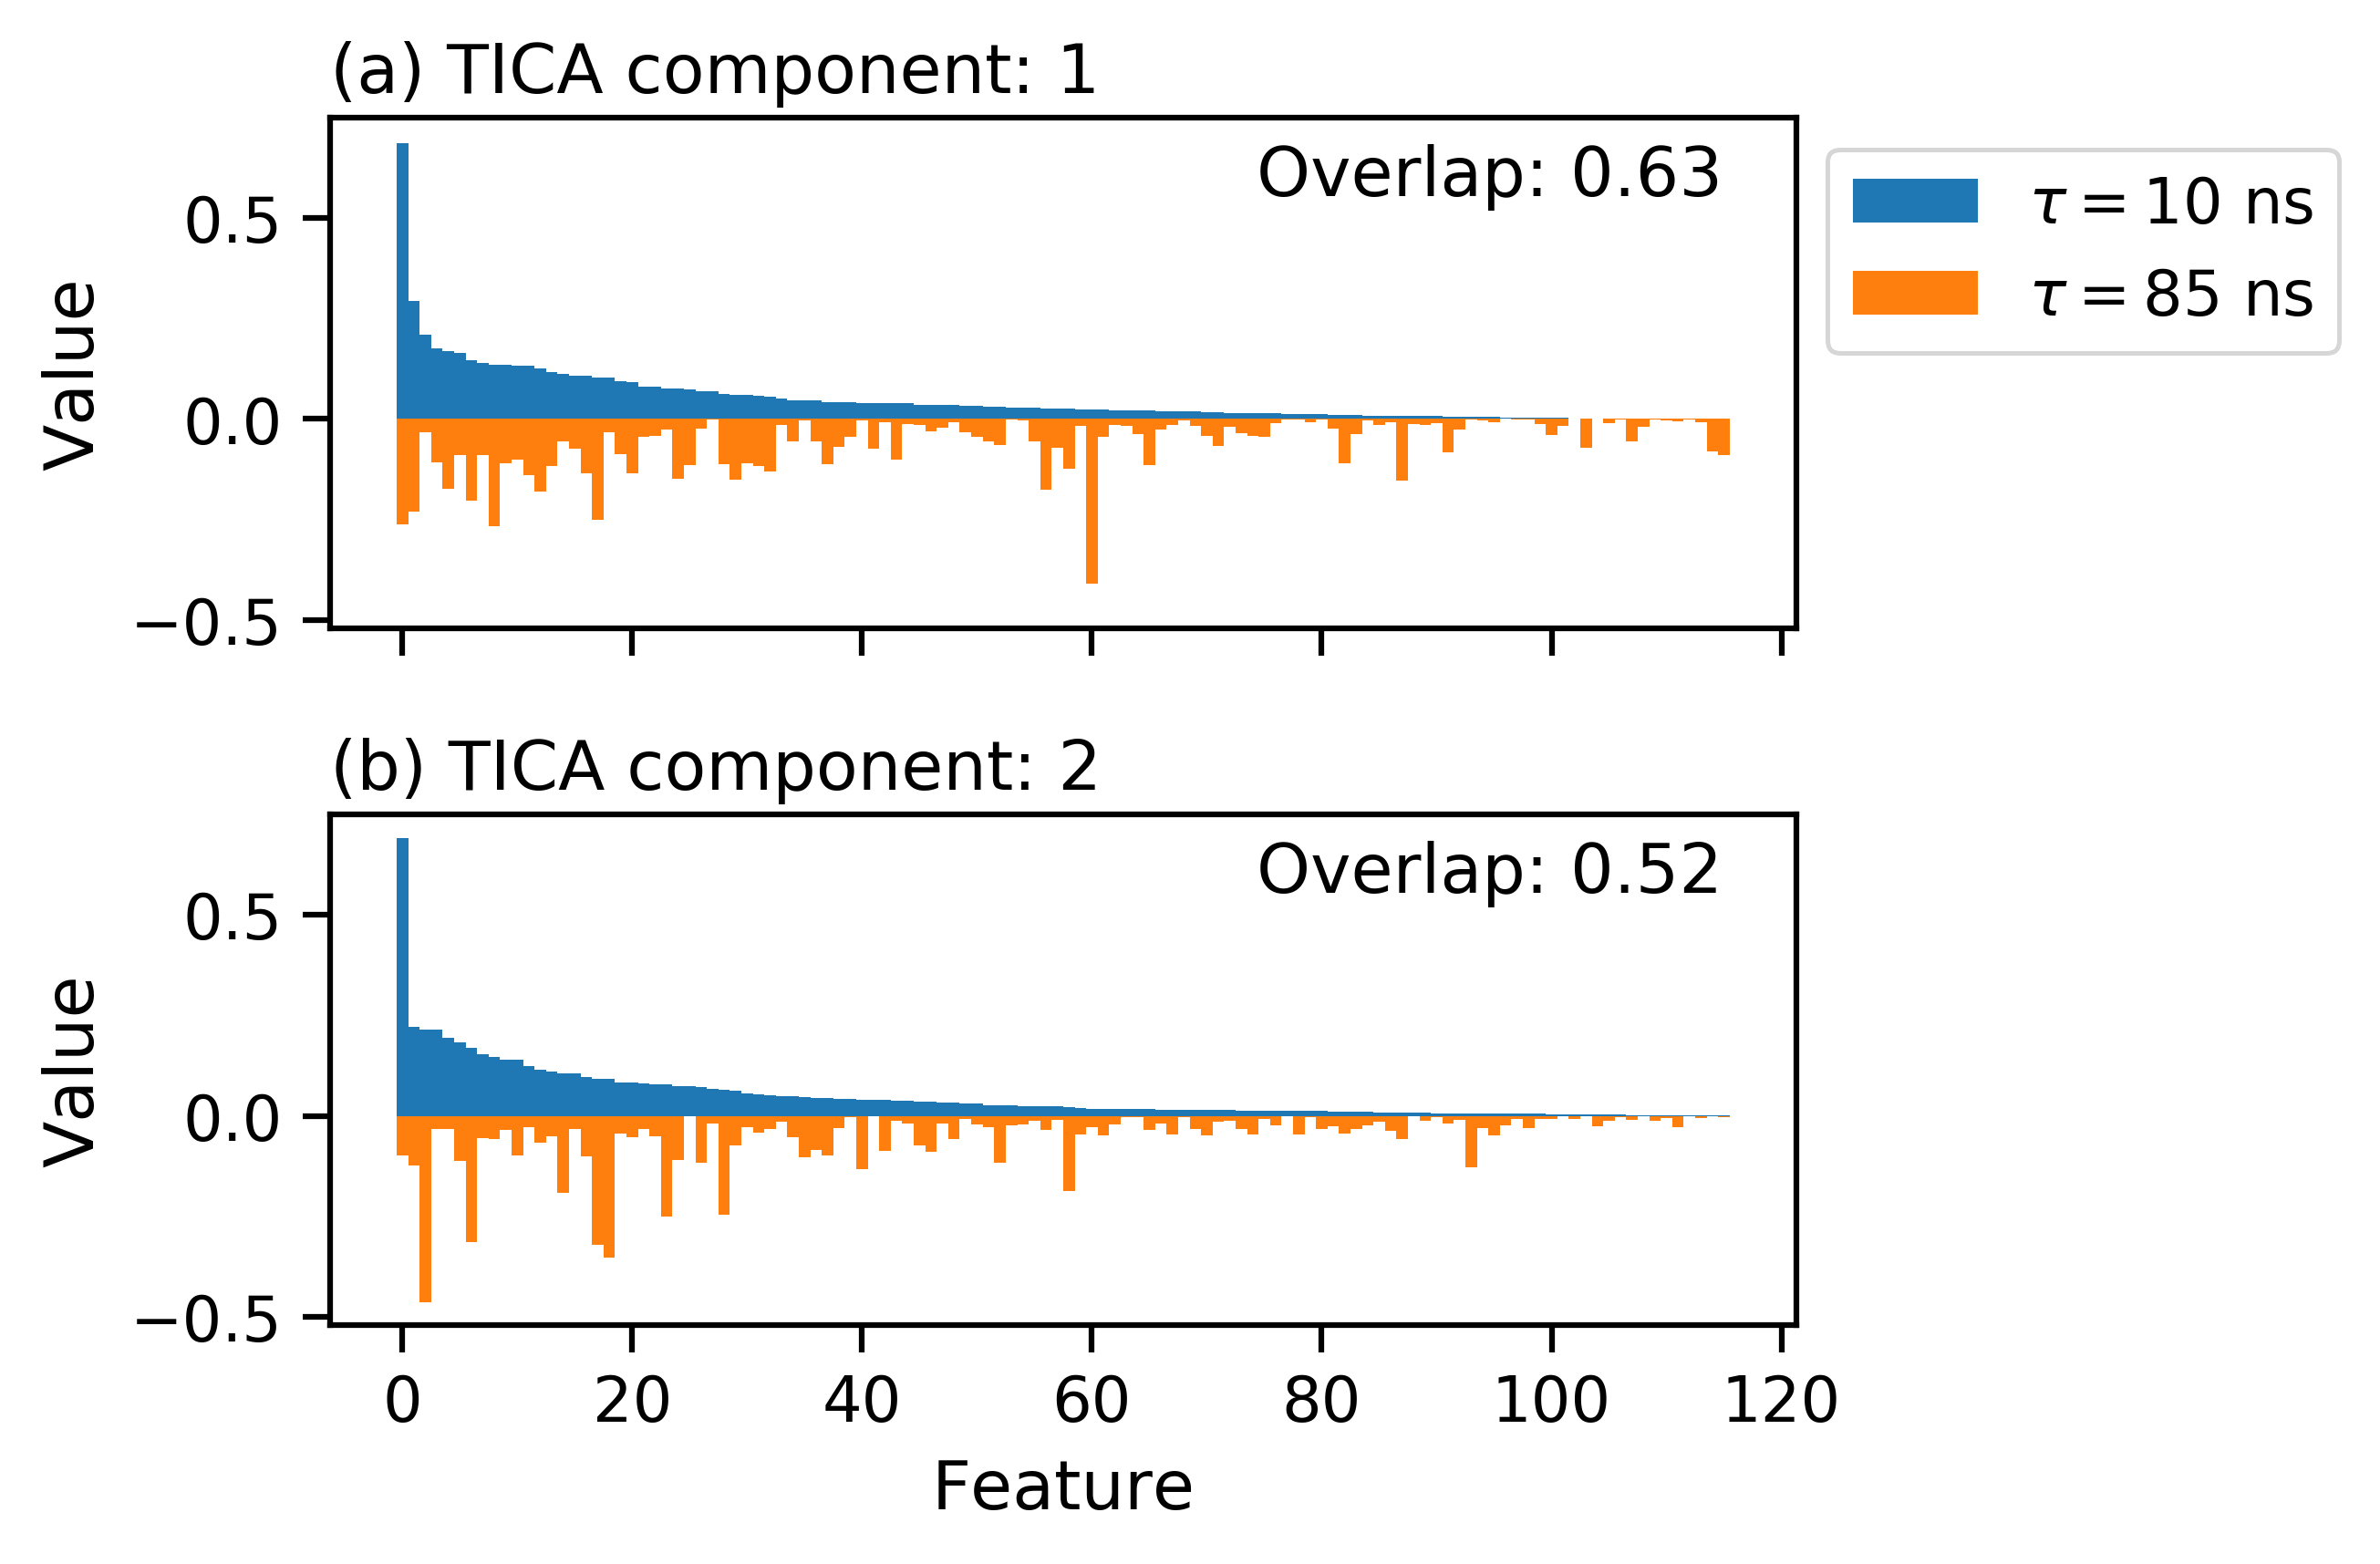
\includegraphics[width=0.8\textwidth]{chapters/msm_optimization/figures/aadh_msm_sens_3_tica.png}
    \label{fig:aadh_msm_sens_3_tica}
\end{figure}


\section{Conclusions}

This chapter demonstrated the use of response surfaces and Bayesian optimisation for understanding and optimizing the hyper-parameters of an MSMs with the following method. The response of an MSM to a randomly selected set of hyper-parameters was measured using standard the MSM metric, VAMP-2. These data were used with Gaussian process regression (GPR) to model the response surface of the MSM. Input warping and the type of kernel used in the  GPR were chosen using cross-validation of the standardised log loss and squared error metrics.  Bayesian optimisation was used to find the optimum of the response surface using the expected improvement as a hyper-parameter selection policy. Once the optimum had been found and the corresponding MSM was estimated, the response surface and eigenvalue spectrum was used to explore the robustness of the optimum hyper-parameters with a series of sensitivity tests. 

Parts of this method was first trialled on the case of alanine dipeptide with a two hyper-parameter response surface. Despite the non-stationary nature of the response surface a GPR with stationary kernels was able to fit the observed data well. The GPR fitting process was seen to be simple and computationally feasible, even with 100s of observations, using recently developed approximations to the full covariance matrix of the GP. The response surface was almost solely a function of the feature (with only a slight dependence on the number of microstates for the two best performing features) and the GP kernel hyper-parameters, the \emph{relevances} of the individual kernel functions, reflected this. The irrelevance of $n$ was suggested as being due to the small number of eigenvectors which were rapidly well approximated with approximately $100$ microstates. For large $n$ the large amount of simulation data meant over-fitting did not become a problem. These two features combined to render to a flat response of the MSM to values of $n$. 

Bayesian optimisation was also trialled on the alanine dipeptide system to determine a suitable number of observations per MSM hyper-parameter, $p$. The optimisation trials did not strongly suggest a particular value of $p$ as the response surface did not improve significantly on any optimisation run. This was due the irrelevance of $n$ and the two identical maxima (at $\chi=(\phi, \psi)$ torsions and the heavy atom positions).  This resulted in an overly simplistic surface which was easily optimized with just random trial data. Problems with fitting the GPR of such a surface in a low data case ($p=15$) were indicated as the incumbent actually decreased in some of the optimisation runs, as a result a value of $p=25$ was used. 

A response surface was fit






\section{Appendix}\label{app:msm_opt}

\subsection{Alanine Dipeptide}

\begin{figure}[h!]
    \centering
    \caption{The $\operatorname{VAMP-2}$ scores of the hyperparameter trials for MSMs of alanine dipeptide. The test response, $f^{test} = f(\chi, n; x^{test})$ is shown in blue, panels: a, c, e, g, i,  while the degree of over-fitting, $f^{train} - f^{test}$, is shown in orange, panels: b, d, f, h, j. Each row represents a different value of the feature ($\chi$) and the horizontal axis represent the number of clusters, ($n$). Each trial was scored with $20$ iterations of 50:50 shuffle split cross validation. The error bars represent the $25$th and $75$th quantiles of the cross-validation folds. 
    The features are ordered according to the mean of the their test scores.}
    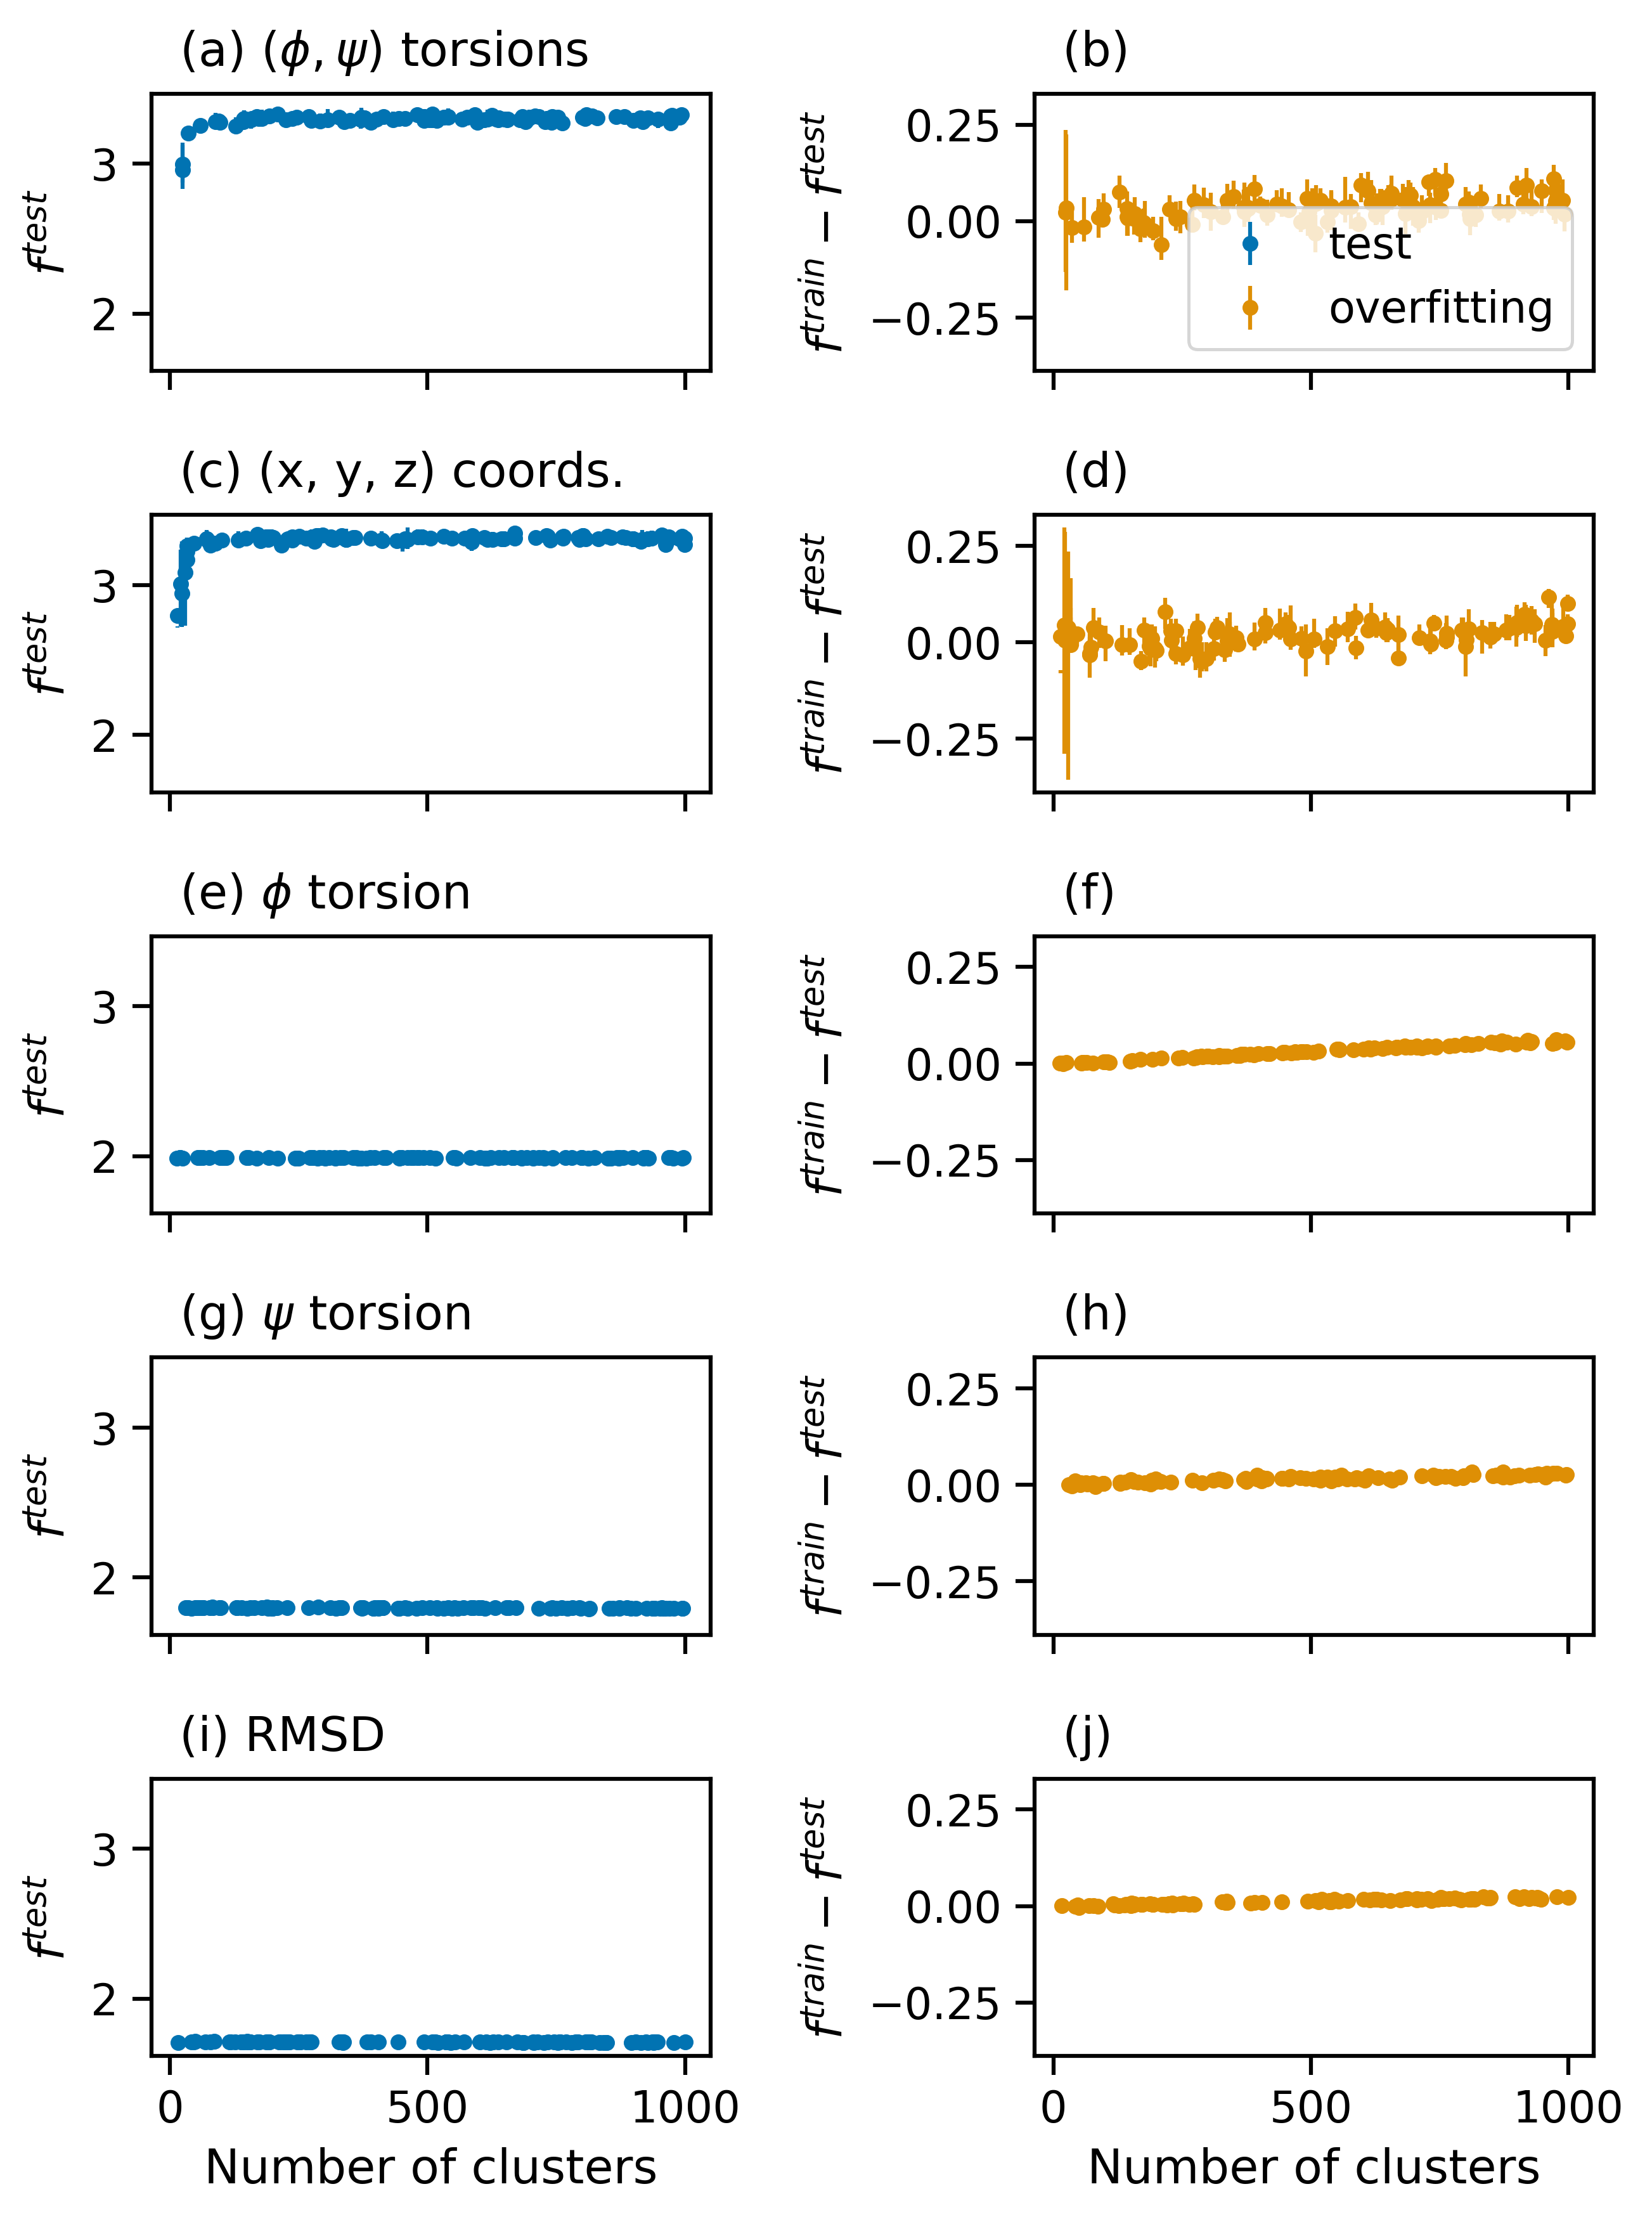
\includegraphics[height=0.8\textheight]{chapters/msm_optimization/figures/ala1_train_test_results.png}
    \label{fig:ala1_train_test}
\end{figure}

\begin{table}[h]
    \centering
    \caption{ Model selection metrics othe response surface of Alanine Dipeptide. Standardised mean square error (SMSE) and mean standardised log loss (MSLL) for GP models of the response surface of MSMs for alanine dipeptide, using different transformations of $n$ ($T(n)$) and different kernels. Each GP model used a mean prior of zero, and all other parameters were estimated by maximizing the marginal likelihood. All values were calculated using 10-fold cross-validation.}
    \begin{tabular}{|l|l|c|c|c|}
    \hline
    T(n) &       Name &  SMSE &    MSLL \\
    \hline\hline
     $\log{(n)}$ &  Exponential & 0.0012 & -3.9963 \\
      &  Mat{\'e}rn 3-2  & 0.0010 & -4.1712 \\
      &  Mat{\'e}rn 5-2  & 0.0007 & -4.2369 \\
      &  Gaussian & 0.0011 & -4.0892 \\
     $I(n)$ &  Exponential  & 0.0027 & -2.9733 \\
      &  Mat{\'e}rn 3-2  & 0.0025 & -3.4218 \\
      &  Mat{\'e}rn 5-2  & 0.0023 & -3.8172 \\
      &  Gaussian & 0.0032 & -4.1239 \\
    \hline
    \end{tabular}
    \label{tab:ala2_fit_results}
\end{table}

\begin{figure}
    \centering
    \caption{Caption}
    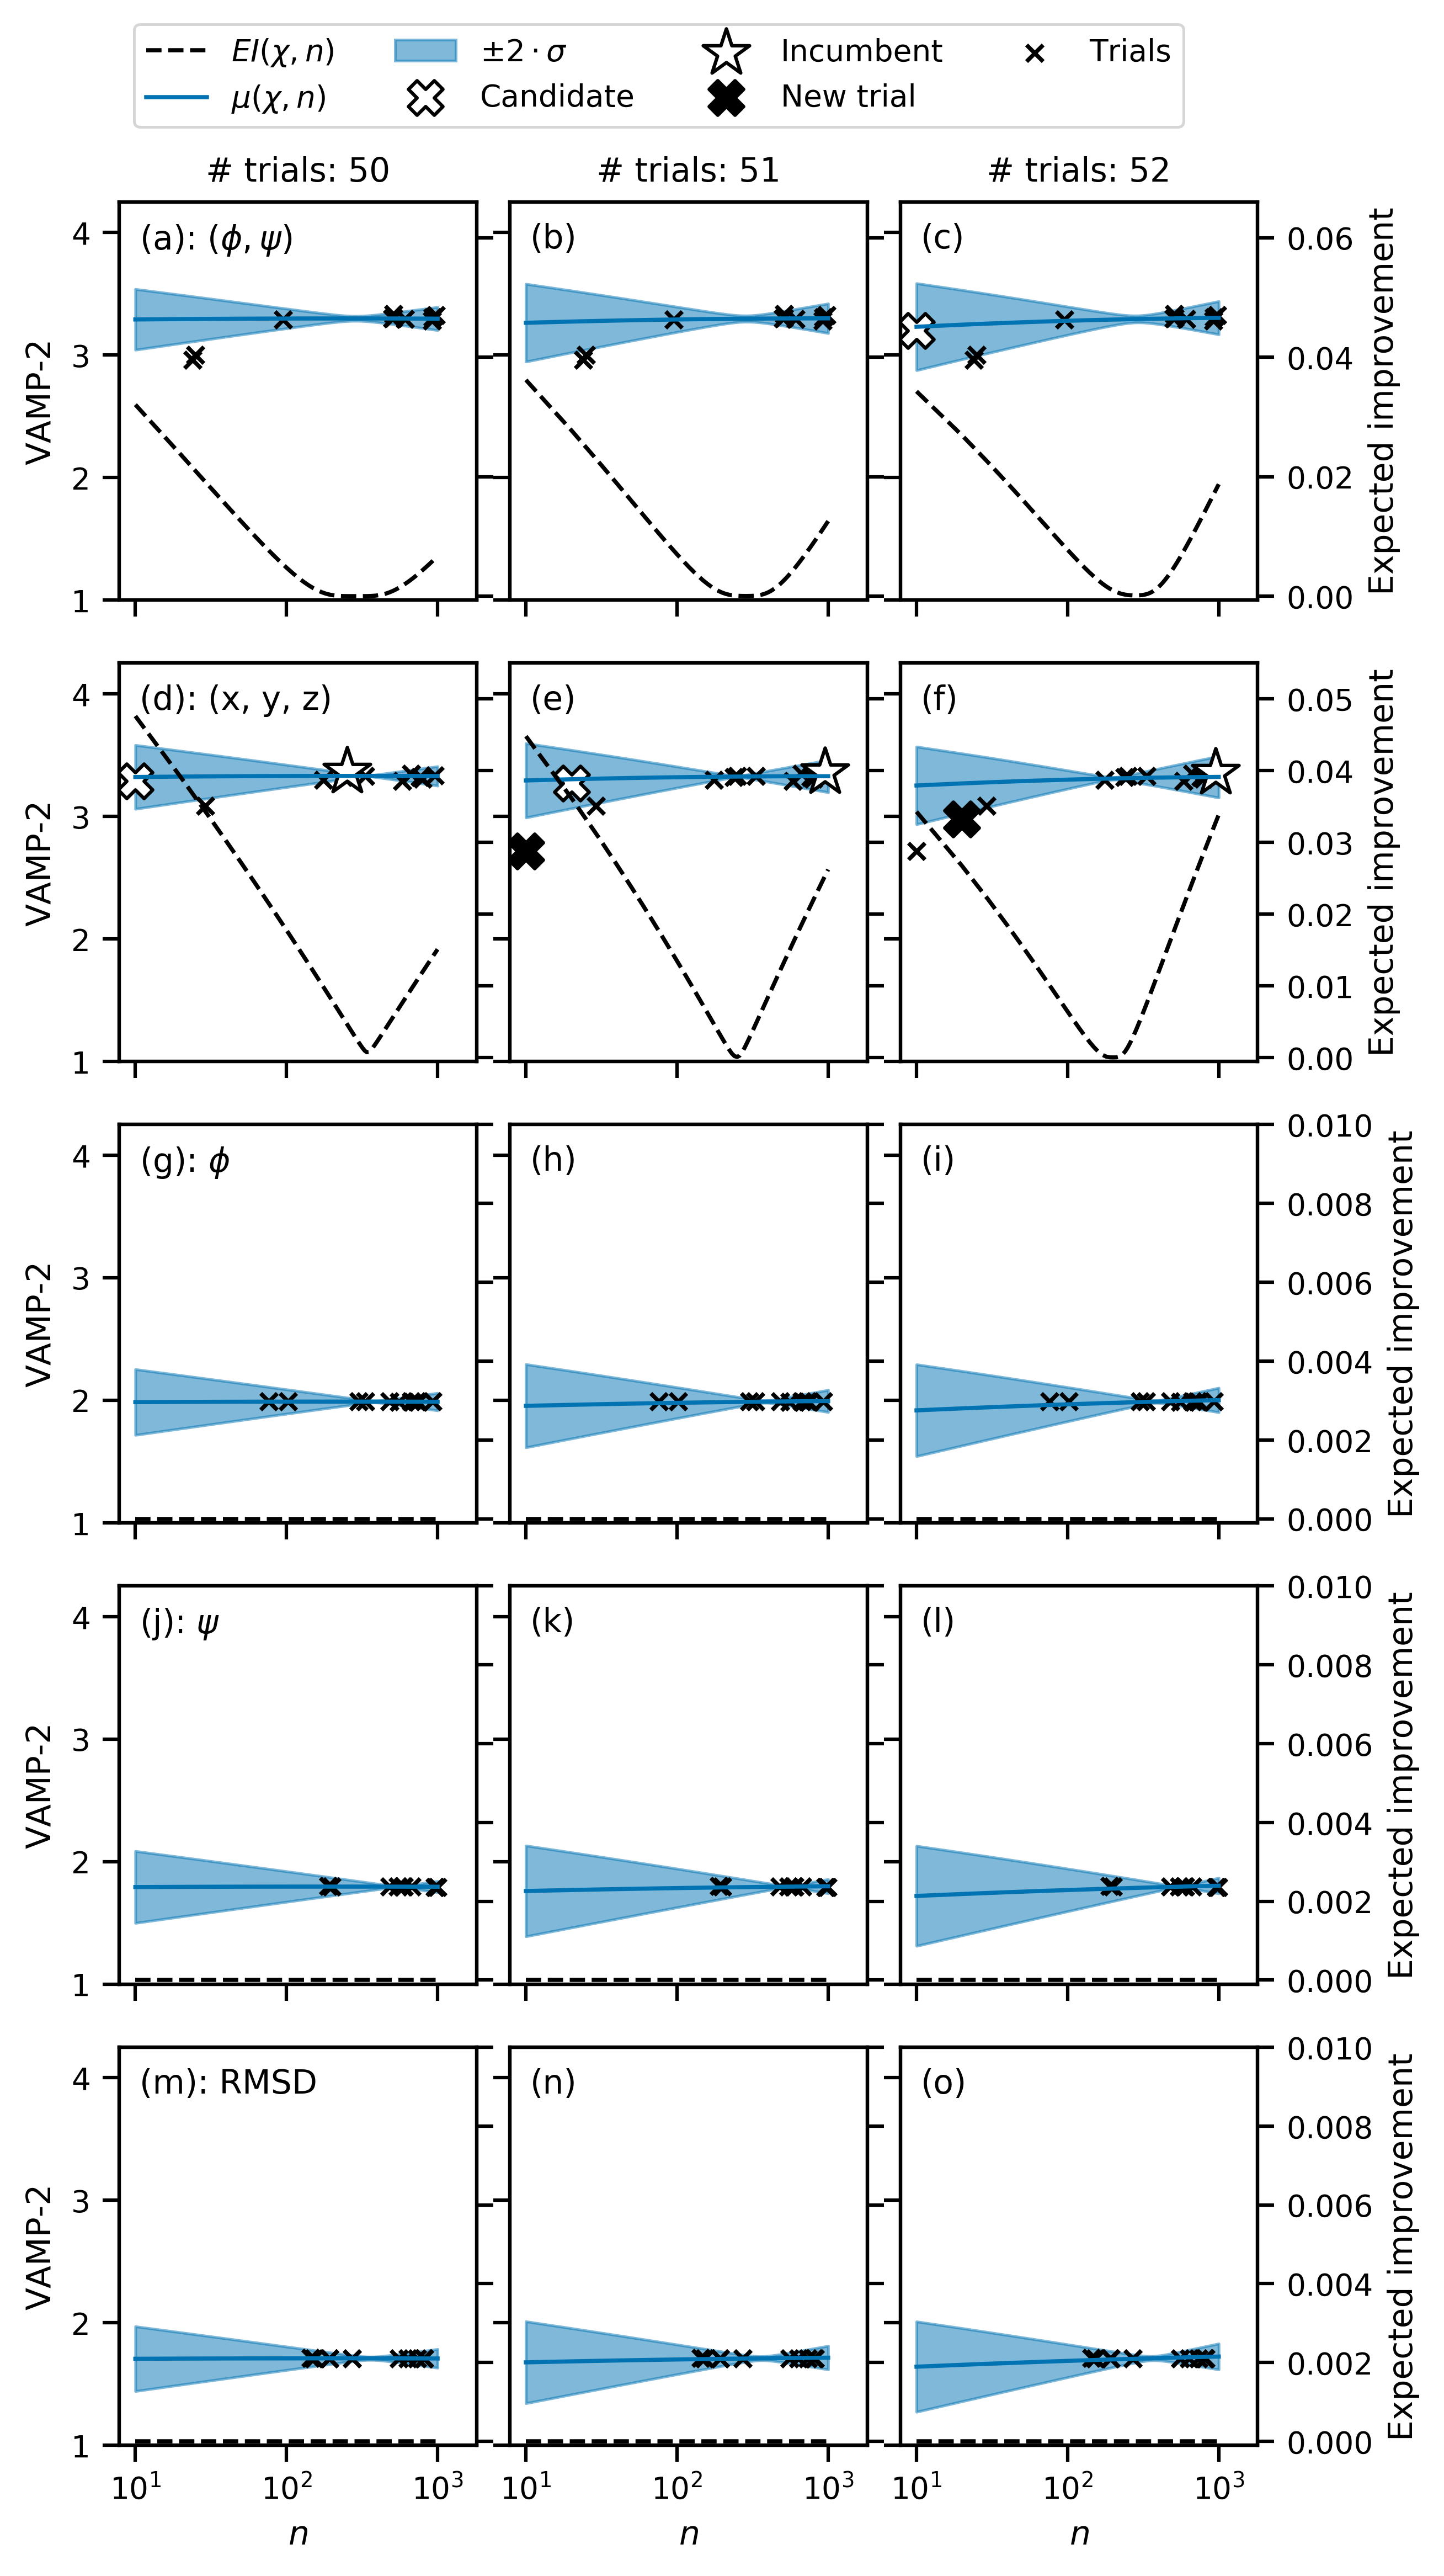
\includegraphics[height=0.8\textheight]{chapters/msm_optimization/figures/ala1_opt_explainer.png}
    \label{fig:ala1_opt_expl}
\end{figure}

\subsection{AADH}

\begin{figure}
    \centering
    \caption{The $\operatorname{VAMP-2}$ scores of the hyperparameter trials for MSMs of AADH with featurised with (a) the $\phi, \psi, \chi$ torsions, (b) all distances between heavy atoms, (c) alpha-Carbon contact distances, (d) heavy atom contact distances, (e) root mean square deviation of heavy atoms. The trials are scored on the test set (blue) and on the training set (orange) for the H active site. The horizontal axis is the rank of the trial according to the test score. Each trial was scored with 20 iterations of 50:50 shuffle split cross validation. The error bars represent the 25th and 75th quantiles of the cross-validation folds. The features are ordered according to the mean of the their test scores.}
    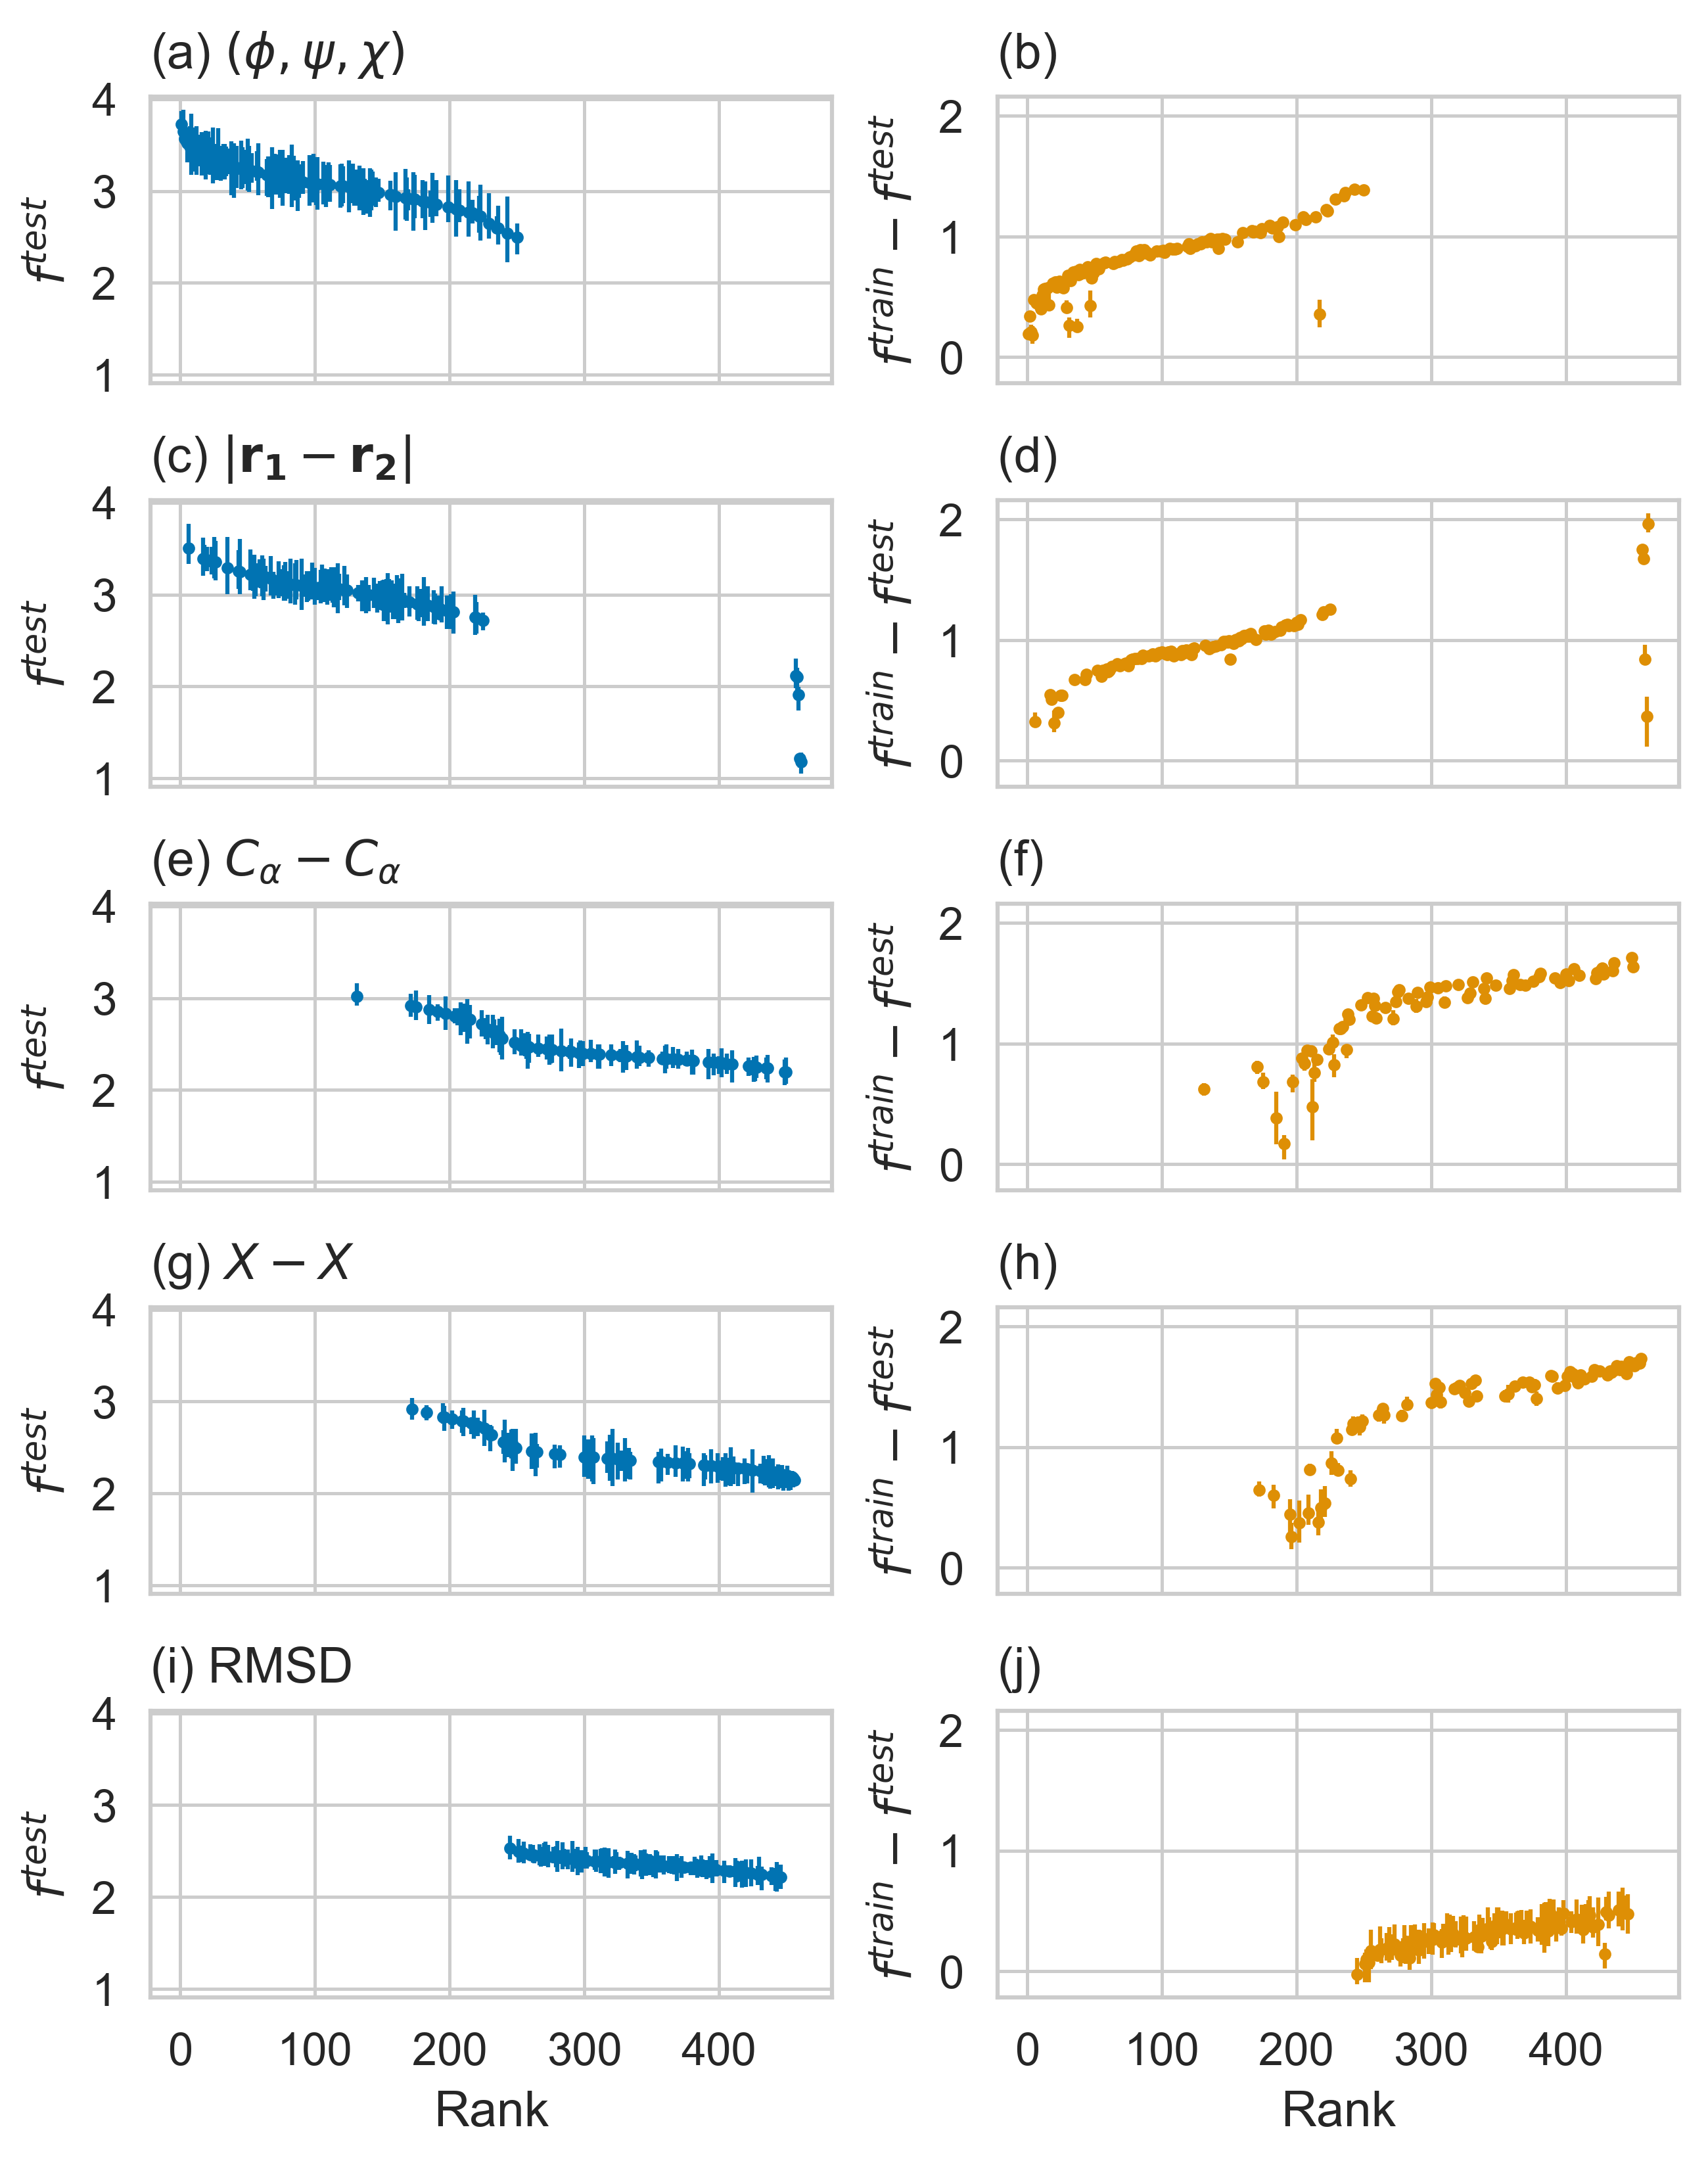
\includegraphics[width=0.8\textwidth]{chapters/msm_optimization/figures/aadh_train_test_results.png}
    \label{fig:aad_train_test}
\end{figure}



\begin{table}
    \centering
    \caption{Model selection metrics for the response surface of AADH using all hyperparameter trials ($N=361$, except those for $\chi=$RMSD). The Mean Standardised Log Loss (MSLL) and Standardised Mean Square Error (SMSE) where calculated using 10 fold cross validation. Only those models which had both $\mathrm{MSLL}<0$ and $\mathrm{SMSE}<1$ were ranked. The total rank is calculated as rank of $\sqrt{R_{MSLL}^{2}+R_{SMSE}^2}$. Where the overall rank was tied, the first model appearing in the table was ranked higher. }
    \label{tab:aadh_rsm_metrics_all_data}
    \begin{tabularx}{1\textwidth}{|llllrr >{\raggedright\arraybackslash}X>{\raggedright\arraybackslash}X>{\raggedright\arraybackslash}X|}
    \hline
    $T(\tau)$ & $T(m)$ & $T(n)$ & Kernel & MSLL &   SMSE & Rank (MSLL) & Rank (SMSE) & Rank (Total)\\
    \hline\hline
    $I({\tau})$ & $I({m})$ & $I({n})$ & Exponential & -0.1298 & 0.3087 &       1.0 &       1.0 &  1.0 \\
                   &             & $\log({n})$ & Exponential &  0.0050 & 0.2964 &         - &         - &    - \\
                   & $\log({m})$ & $I({n})$ & Exponential &  0.0521 & 0.3118 &         - &         - &    - \\
                   &             & $\log({n})$ & Exponential &  0.5633 & 0.3815 &         - &         - &    - \\
    $\log({\tau})$ & $I({m})$ & $I({n})$ & Exponential &  0.1967 & 0.3436 &         - &         - &    - \\
                   &             & $\log({n})$ & Exponential &  0.4959 & 0.3231 &         - &         - &    - \\
                   & $\log({m})$ & $I({n})$ & Exponential &  0.5128 & 0.4365 &         - &         - &    - \\
                   &             & $\log({n})$ & Exponential &  1.0267 & 0.4201 &         - &         - &    - \\
    $I({\tau})$ & $I({m})$ & $I({n})$ & M32 &  1.5680 & 0.2893 &         - &         - &    - \\
                   &             & $\log({n})$ & M32 &  1.9193 & 0.2960 &         - &         - &    - \\
                   & $\log({m})$ & $I({n})$ & M32 &  3.1385 & 0.2775 &         - &         - &    - \\
                   &             & $\log({n})$ & M32 &  2.0358 & 0.2818 &         - &         - &    - \\
    $\log({\tau})$ & $I({m})$ & $I({n})$ & M32 &  6.9015 & 0.3203 &         - &         - &    - \\
                   &             & $\log({n})$ & M32 &  7.7182 & 0.3406 &         - &         - &    - \\
                   & $\log({m})$ & $I({n})$ & M32 &  7.9209 & 0.3257 &         - &         - &    - \\
                   &             & $\log({n})$ & M32 &  3.0002 & 0.3472 &         - &         - &    - \\
    $I({\tau})$ & $I({m})$ & $I({n})$ & M52 &  3.6517 & 0.3029 &         - &         - &    - \\
                   &             & $\log({n})$ & M52 &  3.8316 & 0.3090 &         - &         - &    - \\
                   & $\log({m})$ & $I({n})$ & M52 &  8.6574 & 0.2991 &         - &         - &    - \\
                   &             & $\log({n})$ & M52 &  3.7354 & 0.3238 &         - &         - &    - \\
    $\log({\tau})$ & $I({m})$ & $I({n})$ & M52 &  8.9207 & 0.3679 &         - &         - &    - \\
                   &             & $\log({n})$ & M52 & 11.8753 & 0.4064 &         - &         - &    - \\
                   & $\log({m})$ & $I({n})$ & M52 & 12.7637 & 0.3722 &         - &         - &    - \\
                   &             & $\log({n})$ & M52 & 13.6735 & 0.3475 &         - &         - &    - \\
    $I({\tau})$ & $I({m})$ & $I({n})$ & RBF &     inf &    inf &         - &         - &    - \\
                   &             & $\log({n})$ & RBF &  9.3618 & 0.3256 &         - &         - &    - \\
                   & $\log({m})$ & $I({n})$ & RBF &  5.9123 & 0.3022 &         - &         - &    - \\
                   &             & $\log({n})$ & RBF &     inf &    inf &         - &         - &    - \\
    $\log({\tau})$ & $I({m})$ & $I({n})$ & RBF & 17.4786 & 0.4551 &         - &         - &    - \\
                   &             & $\log({n})$ & RBF & 16.7568 & 0.3556 &         - &         - &    - \\
                   & $\log({m})$ & $I({n})$ & RBF & 16.7412 & 0.5026 &         - &         - &    - \\
                   &             & $\log({n})$ & RBF & 24.3199 & 0.4986 &         - &         - &    - \\
    \hline
    \end{tabularx}
\end{table}

\begin{figure}[ht]
    \centering
    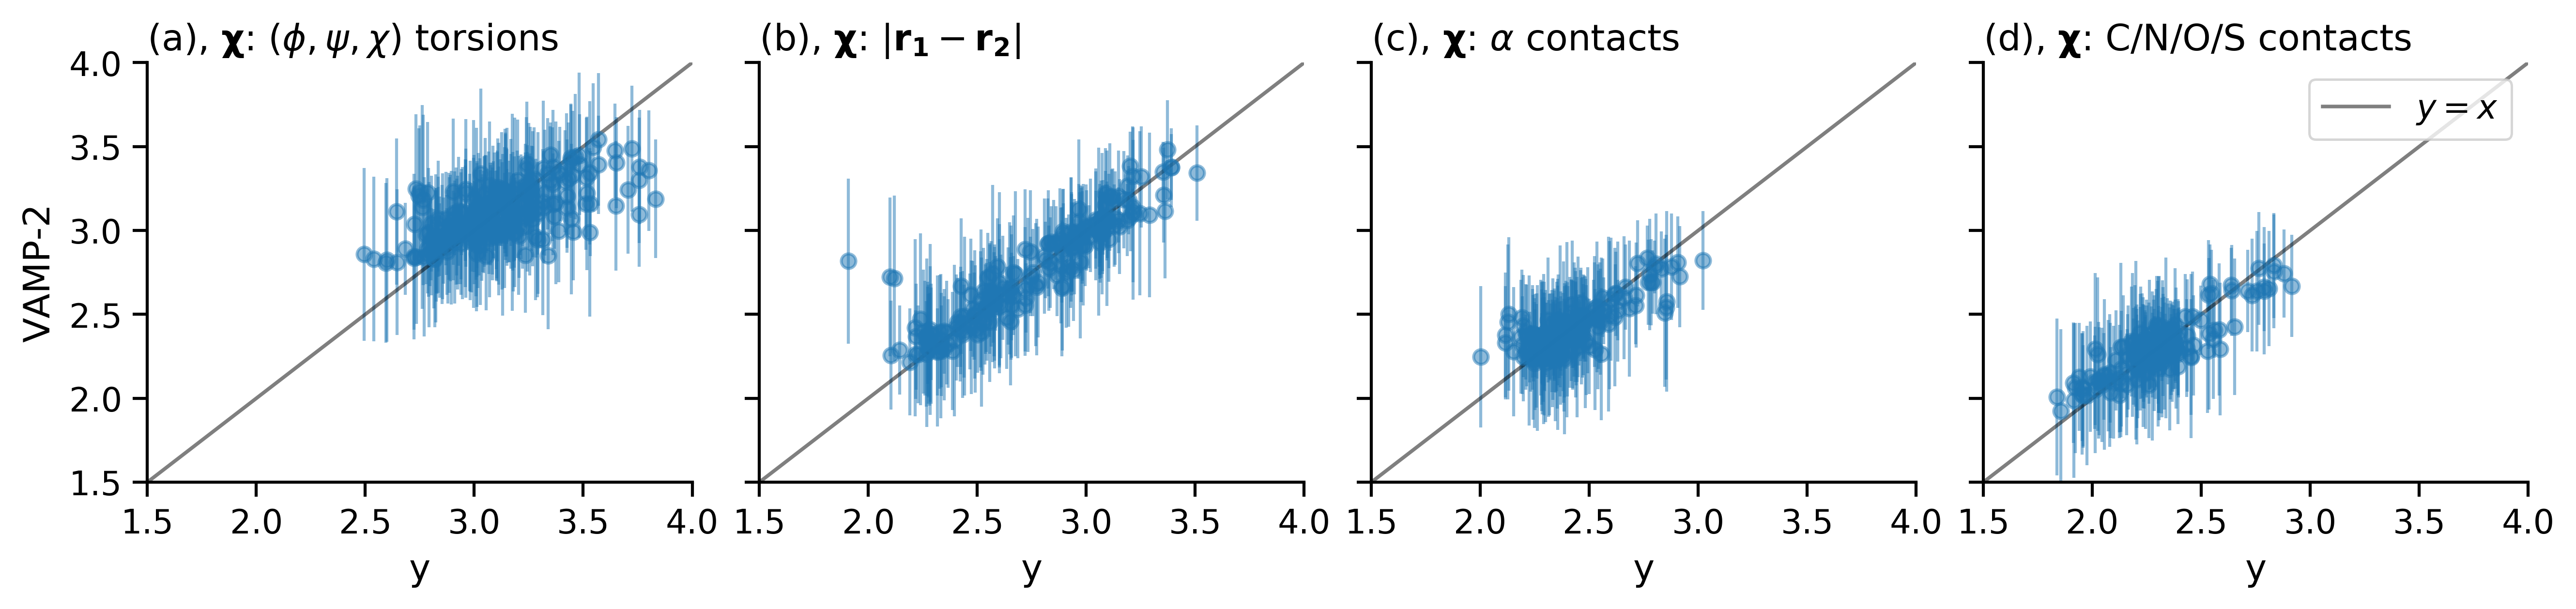
\includegraphics[width=0.8\textwidth]{chapters/msm_optimization/figures/aadh_response_surface_fit_d.png}
    \caption{Caption}
    \label{fig:aadh_rsm_fit}
\end{figure}


\begin{table}
    \centering
    \caption{Model selection metrics for the response surface of an MSM of AADH, data subset 1, $N=100$, except those for $\chi=$RMSD). The Mean Standardised Log Loss (MSLL) and Standardised Mean Square Error (SMSE) where calculated using 10 fold cross validation. Only those models which had both $\mathrm{MSLL}<0$ and $\mathrm{SMSE}<1$ were ranked. The total rank is calculated as rank of $\sqrt{R_{MSLL}^{2}+R_{SMSE}^2}$. Where the overall rank was tied, the first model appearing in the table was ranked higher. }
    \label{tab:aadh_rsm_metrics_iter_1}
    \begin{tabularx}{1\textwidth}{|llllrr >{\raggedright\arraybackslash}X>{\raggedright\arraybackslash}X>{\raggedright\arraybackslash}X|}
    \hline
    $T(\tau)$ & $T(m)$ & $T(n)$ & Kernel & MSLL &   SMSE & Rank (MSLL) & Rank (SMSE) & Rank (Total)\\
    \hline\hline
    $I({\tau})$ & $I({m})$ & $I({n})$ & Exponential & -0.3928 & 0.3412 &        10.0 &        14.0 &         13.0 \\
               &             & $\log({n})$ & Exponential & -0.2456 & 0.3443 &        15.0 &        15.0 &         16.0 \\
               & $\log({m})$ & $I({n})$ & Exponential & -0.6484 & 0.3169 &         6.0 &        12.0 &          7.0 \\
               &             & $\log({n})$ & Exponential & -0.5585 & 0.3487 &         7.0 &        17.0 &         14.0 \\
    $\log({\tau})$ & $I({m})$ & $I({n})$ & Exponential &  0.0598 & 0.3483 &           - &           - &            - \\
                   &             & $\log({n})$ & Exponential & -0.2195 & 0.3450 &        16.0 &        16.0 &         17.0 \\
                   & $\log({m})$ & $I({n})$ & Exponential & -0.3524 & 0.3084 &        13.0 &         9.0 &         10.0 \\
                   &             & $\log({n})$ & Exponential & -0.3944 & 0.3379 &         9.0 &        13.0 &         11.0 \\
    $I({\tau})$ & $I({m})$ & $I({n})$ & M32 & -0.3807 & 0.3167 &        12.0 &        11.0 &         12.0 \\
                   &             & $\log({n})$ & M32 & -0.2744 & 0.3053 &        14.0 &         7.0 &          9.0 \\
                   & $\log({m})$ & $I({n})$ & M32 & -0.8769 & 0.2779 &         1.0 &         4.0 &          3.0 \\
                   &             & $\log({n})$ & M32 & -0.7438 & 0.2785 &         5.0 &         5.0 &          5.0 \\
    $\log({\tau})$ & $I({m})$ & $I({n})$ & M32 &  0.3415 & 0.3721 &           - &           - &            - \\
                   &             & $\log({n})$ & M32 & -0.2023 & 0.3892 &        17.0 &        18.0 &         18.0 \\
                   & $\log({m})$ & $I({n})$ & M32 & -0.4758 & 0.3033 &         8.0 &         6.0 &          6.0 \\
                   &             & $\log({n})$ & M32 & -0.3892 & 0.3086 &        11.0 &        10.0 &          8.0 \\
    $I({\tau})$ & $I({m})$ & $I({n})$ & M52 &  0.3362 & 0.3149 &           - &           - &            - \\
                   &             & $\log({n})$ & M52 &  0.9964 & 0.2712 &           - &           - &            - \\
                   & $\log({m})$ & $I({n})$ & M52 & -0.8713 & 0.2685 &         2.0 &         2.0 &          1.0 \\
                   &             & $\log({n})$ & M52 & -0.7508 & 0.2700 &         4.0 &         3.0 &          4.0 \\
    $\log({\tau})$ & $I({m})$ & $I({n})$ & M52 &  6.4201 & 0.3503 &           - &           - &            - \\
                   &             & $\log({n})$ & M52 &  5.7695 & 0.3250 &           - &           - &            - \\
                   & $\log({m})$ & $I({n})$ & M52 &  3.9718 & 0.3153 &           - &           - &            - \\
                   &             & $\log({n})$ & M52 &     inf &    inf &           - &           - &            - \\
    $I({\tau})$ & $I({m})$ & $I({n})$ & RBF & -0.1677 & 0.3074 &        18.0 &         8.0 &         15.0 \\
                   &             & $\log({n})$ & RBF &  1.3068 & 0.2747 &           - &           - &            - \\
                   & $\log({m})$ & $I({n})$ & RBF & -0.7884 & 0.2675 &         3.0 &         1.0 &          2.0 \\
                   &             & $\log({n})$ & RBF &     inf &    inf &           - &           - &            - \\
    $\log({\tau})$ & $I({m})$ & $I({n})$ & RBF &  6.8541 & 0.3472 &           - &           - &            - \\
                   &             & $\log({n})$ & RBF &  6.2984 & 0.3074 &           - &           - &            - \\
                   & $\log({m})$ & $I({n})$ & RBF &  4.8742 & 0.4157 &           - &           - &            - \\
                   &             & $\log({n})$ & RBF &  7.6739 & 0.5531 &           - &           - &            - \\
    \hline
    \end{tabularx}
\end{table}

\begin{table}
    \centering
    \caption{Model selection metrics for the response surface of an MSM of AADH, data subset 2, $N=100$, except those for $\chi=$RMSD). The Mean Standardised Log Loss (MSLL) and Standardised Mean Square Error (SMSE) where calculated using 10 fold cross validation. Only those models which had both $\mathrm{MSLL}<0$ and $\mathrm{SMSE}<1$ were ranked. The total rank is calculated as rank of $\sqrt{R_{MSLL}^{2}+R_{SMSE}^2}$. Where the overall rank was tied, the first model appearing in the table was ranked higher. }
    \label{tab:aadh_rsm_metrics_iter_2}
    \begin{tabularx}{1\textwidth}{|llllrr >{\raggedright\arraybackslash}X>{\raggedright\arraybackslash}X>{\raggedright\arraybackslash}X|}
    \hline
    $T(\tau)$ & $T(m)$ & $T(n)$ & Kernel & MSLL &   SMSE & Rank (MSLL) & Rank (SMSE) & Rank (Total)\\
    \hline\hline
    $I({\tau})$ & $I({m})$ & $I({n})$ & Exponential & -0.3293 & 0.4262 &        13.0 &         9.0 &         11.0 \\
                   &             & $\log({n})$ & Exponential & -0.5222 & 0.4330 &         6.0 &        13.0 &          8.0 \\
                   & $\log({m})$ & $I({n})$ & Exponential & -0.6612 & 0.3890 &         1.0 &         2.0 &          1.0 \\
                   &             & $\log({n})$ & Exponential & -0.5843 & 0.4170 &         3.0 &         5.0 &          3.0 \\
    $\log({\tau})$ & $I({m})$ & $I({n})$ & Exponential & -0.3737 & 0.4590 &        11.0 &        15.0 &         15.0 \\
                   &             & $\log({n})$ & Exponential & -0.4162 & 0.4445 &         8.0 &        14.0 &         12.0 \\
                   & $\log({m})$ & $I({n})$ & Exponential & -0.3702 & 0.4281 &        12.0 &        10.0 &         10.0 \\
                   &             & $\log({n})$ & Exponential & -0.6242 & 0.4169 &         2.0 &         4.0 &          2.0 \\
    $I({\tau})$ & $I({m})$ & $I({n})$ & M32 & -0.5737 & 0.4218 &         4.0 &         7.0 &          5.0 \\
                   &             & $\log({n})$ & M32 &  0.1639 & 0.4432 &           - &           - &            - \\
                   & $\log({m})$ & $I({n})$ & M32 & -0.5479 & 0.4282 &         5.0 &        11.0 &          7.0 \\
                   &             & $\log({n})$ & M32 & -0.4595 & 0.3844 &         7.0 &         1.0 &          4.0 \\
    $\log({\tau})$ & $I({m})$ & $I({n})$ & M32 & -0.4077 & 0.4301 &         9.0 &        12.0 &          9.0 \\
                   &             & $\log({n})$ & M32 &     inf &    inf &           - &           - &            - \\
                   & $\log({m})$ & $I({n})$ & M32 &  1.0248 & 0.4609 &           - &           - &            - \\
                   &             & $\log({n})$ & M32 & -0.3902 & 0.3942 &        10.0 &         3.0 &          6.0 \\
    $I({\tau})$ & $I({m})$ & $I({n})$ & M52 &  1.3964 & 0.4033 &           - &           - &            - \\
                   &             & $\log({n})$ & M52 &  0.3681 & 0.4475 &           - &           - &            - \\
                   & $\log({m})$ & $I({n})$ & M52 & -0.1968 & 0.4237 &        14.0 &         8.0 &         13.0 \\
                   &             & $\log({n})$ & M52 &  2.3201 & 0.4400 &           - &           - &            - \\
    $\log({\tau})$ & $I({m})$ & $I({n})$ & M52 &  3.2132 & 0.4125 &           - &           - &            - \\
                   &             & $\log({n})$ & M52 &  0.5430 & 0.4473 &           - &           - &            - \\
                   & $\log({m})$ & $I({n})$ & M52 &  1.6455 & 0.4679 &           - &           - &            - \\
                   &             & $\log({n})$ & M52 &  0.7421 & 0.4378 &           - &           - &            - \\
    $I({\tau})$ & $I({m})$ & $I({n})$ & RBF &  2.3960 & 0.4042 &           - &           - &            - \\
                   &             & $\log({n})$ & RBF &  1.3825 & 0.4372 &           - &           - &            - \\
                   & $\log({m})$ & $I({n})$ & RBF & -0.1688 & 0.4197 &        15.0 &         6.0 &         14.0 \\
                   &             & $\log({n})$ & RBF &  3.8725 & 0.4652 &           - &           - &            - \\
    $\log({\tau})$ & $I({m})$ & $I({n})$ & RBF &  4.1994 & 0.4244 &           - &           - &            - \\
                   &             & $\log({n})$ & RBF &  2.3169 & 0.4305 &           - &           - &            - \\
                   & $\log({m})$ & $I({n})$ & RBF &  1.7600 & 0.4764 &           - &           - &            - \\
                   &             & $\log({n})$ & RBF &  1.6457 & 0.4517 &           - &           - &            - \\
    \hline
    \end{tabularx}
\end{table}


\begin{table}
    \centering
    \caption{Model selection metrics for the response surface of an MSM of AADH, data subset 3, $N=100$, except those for $\chi=$RMSD). The Mean Standardised Log Loss (MSLL) and Standardised Mean Square Error (SMSE) where calculated using 10 fold cross validation. Only those models which had both $\mathrm{MSLL}<0$ and $\mathrm{SMSE}<1$ were ranked. The total rank is calculated as rank of $\sqrt{R_{MSLL}^{2}+R_{SMSE}^2}$. Where the overall rank was tied, the first model appearing in the table was ranked higher. }
    \label{tab:aadh_rsm_metrics_iter_3}
    \begin{tabularx}{1\textwidth}{|llllrr >{\raggedright\arraybackslash}X>{\raggedright\arraybackslash}X>{\raggedright\arraybackslash}X|}
    \hline
    $T(\tau)$ & $T(m)$ & $T(n)$ & Kernel & MSLL &   SMSE & Rank (MSLL) & Rank (SMSE) & Rank (Total)\\
    \hline\hline
    $I({\tau})$ & $I({m})$ & $I({n})$ & Exponential & -0.4461 & 0.5415 &        14.0 &        15.0 &         13.0 \\
                   &             & $\log({n})$ & Exponential & -0.4350 & 0.5234 &        15.0 &         9.0 &         10.0 \\
                   & $\log({m})$ & $I({n})$ & Exponential & -0.6123 & 0.5074 &         6.0 &         5.0 &          3.0 \\
                   &             & $\log({n})$ & Exponential & -0.5378 & 0.5145 &         9.0 &         7.0 &          5.0 \\
    $\log({\tau})$ & $I({m})$ & $I({n})$ & Exponential & -0.3138 & 0.6006 &        21.0 &        25.0 &         24.0 \\
                   &             & $\log({n})$ & Exponential & -0.3559 & 0.5626 &        20.0 &        21.0 &         22.0 \\
                   & $\log({m})$ & $I({n})$ & Exponential & -0.4587 & 0.5449 &        13.0 &        17.0 &         14.0 \\
                   &             & $\log({n})$ & Exponential & -0.4276 & 0.5472 &        18.0 &        18.0 &         20.0 \\
    $I({\tau})$ & $I({m})$ & $I({n})$ & M32 & -0.6003 & 0.5234 &         7.0 &         8.0 &          4.0 \\
                   &             & $\log({n})$ & M32 & -0.6400 & 0.5376 &         5.0 &        12.0 &          8.0 \\
                   & $\log({m})$ & $I({n})$ & M32 & -0.8017 & 0.4885 &         2.0 &         1.0 &          1.0 \\
                   &             & $\log({n})$ & M32 & -0.8921 & 0.4892 &         1.0 &         2.0 &          2.0 \\
    $\log({\tau})$ & $I({m})$ & $I({n})$ & M32 & -0.1904 & 0.5933 &        24.0 &        24.0 &         25.0 \\
                   &             & $\log({n})$ & M32 & -0.4898 & 0.5711 &        11.0 &        22.0 &         18.0 \\
                   & $\log({m})$ & $I({n})$ & M32 & -0.4295 & 0.5379 &        17.0 &        13.0 &         15.0 \\
                   &             & $\log({n})$ & M32 & -0.6808 & 0.5350 &         4.0 &        11.0 &          6.0 \\
    $I({\tau})$ & $I({m})$ & $I({n})$ & M52 & -0.4328 & 0.5482 &        16.0 &        19.0 &         19.0 \\
                   &             & $\log({n})$ & M52 & -0.5392 & 0.5262 &         8.0 &        10.0 &          7.0 \\
                   & $\log({m})$ & $I({n})$ & M52 & -0.7498 & 0.5506 &         3.0 &        20.0 &         12.0 \\
                   &             & $\log({n})$ & M52 & -0.2438 & 0.5141 &        22.0 &         6.0 &         16.0 \\
    $\log({\tau})$ & $I({m})$ & $I({n})$ & M52 &  0.4797 & 0.6354 &           - &           - &            - \\
                   &             & $\log({n})$ & M52 & -0.3604 & 0.6100 &        19.0 &        26.0 &         23.0 \\
                   & $\log({m})$ & $I({n})$ & M52 & -0.1492 & 0.5818 &        25.0 &        23.0 &         26.0 \\
                   &             & $\log({n})$ & M52 &  0.1426 & 0.5263 &           - &           - &            - \\
    $I({\tau})$ & $I({m})$ & $I({n})$ & RBF & -0.5234 & 0.5412 &        10.0 &        14.0 &          9.0 \\
                   &             & $\log({n})$ & RBF & -0.4854 & 0.5436 &        12.0 &        16.0 &         11.0 \\
                   & $\log({m})$ & $I({n})$ & RBF &     inf &    inf &           - &           - &            - \\
                   &             & $\log({n})$ & RBF & -0.1291 & 0.5002 &        26.0 &         3.0 &         21.0 \\
    $\log({\tau})$ & $I({m})$ & $I({n})$ & RBF &  1.5339 & 0.5471 &           - &           - &            - \\
                   &             & $\log({n})$ & RBF & -0.0794 & 0.6378 &        27.0 &        27.0 &         27.0 \\
                   & $\log({m})$ & $I({n})$ & RBF & -0.2000 & 0.5068 &        23.0 &         4.0 &         17.0 \\
                   &             & $\log({n})$ & RBF &  0.1399 & 0.4935 &           - &           - &            - \\
    \hline
    \end{tabularx}
\end{table}


\begin{table}
    \centering
    \caption{Model selection metrics for the response surface of an MSM of AADH, data subset 4, $N=100$, except those for $\chi=$RMSD). The Mean Standardised Log Loss (MSLL) and Standardised Mean Square Error (SMSE) where calculated using 10 fold cross validation. Only those models which had both $\mathrm{MSLL}<0$ and $\mathrm{SMSE}<1$ were ranked. The total rank is calculated as rank of $\sqrt{R_{MSLL}^{2}+R_{SMSE}^2}$. Where the overall rank was tied, the first model appearing in the table was ranked higher. }
    \label{tab:aadh_rsm_metrics_iter_4}
    \begin{tabularx}{1\textwidth}{|llllrr >{\raggedright\arraybackslash}X>{\raggedright\arraybackslash}X>{\raggedright\arraybackslash}X|}
    \hline
    $T(\tau)$ & $T(m)$ & $T(n)$ & Kernel & MSLL &   SMSE & Rank (MSLL) & Rank (SMSE) & Rank (Total)\\
    \hline\hline
    $I({\tau})$ & $I({m})$ & $I({n})$ & Exponential & -0.7560 & 0.2203 &         8.0 &        16.0 &         16.0 \\
                   &             & $\log({n})$ & Exponential & -0.7875 & 0.2181 &         7.0 &        15.0 &         15.0 \\
                   & $\log({m})$ & $I({n})$ & Exponential & -0.9947 & 0.1510 &         3.0 &        10.0 &          4.0 \\
                   &             & $\log({n})$ & Exponential & -0.9846 & 0.1449 &         4.0 &         9.0 &          3.0 \\
    $\log({\tau})$ & $I({m})$ & $I({n})$ & Exponential & -0.8015 & 0.2132 &         6.0 &        14.0 &         12.0 \\
                   &             & $\log({n})$ & Exponential & -0.8752 & 0.1825 &         5.0 &        13.0 &          7.0 \\
                   & $\log({m})$ & $I({n})$ & Exponential & -1.0363 & 0.1442 &         1.0 &         8.0 &          2.0 \\
                   &             & $\log({n})$ & Exponential & -1.0279 & 0.1327 &         2.0 &         6.0 &          1.0 \\
    $I({\tau})$ & $I({m})$ & $I({n})$ & M32 &     inf &    inf &           - &           - &            - \\
                   &             & $\log({n})$ & M32 & -0.5648 & 0.1809 &        10.0 &        12.0 &         13.0 \\
                   & $\log({m})$ & $I({n})$ & M32 & -0.4921 & 6.5461 &           - &           - &            - \\
                   &             & $\log({n})$ & M32 & -0.5509 & 0.1001 &        11.0 &         1.0 &          5.0 \\
    $\log({\tau})$ & $I({m})$ & $I({n})$ & M32 & 17.1108 & 4.4912 &           - &           - &            - \\
                   &             & $\log({n})$ & M32 & -0.2896 & 0.1322 &        13.0 &         5.0 &          8.0 \\
                   & $\log({m})$ & $I({n})$ & M32 &  0.8341 & 6.6805 &           - &           - &            - \\
                   &             & $\log({n})$ & M32 & -0.6497 & 0.1530 &         9.0 &        11.0 &          9.0 \\
    $I({\tau})$ & $I({m})$ & $I({n})$ & M52 &  0.0998 & 0.1507 &           - &           - &            - \\
                   &             & $\log({n})$ & M52 &  0.2457 & 0.1419 &           - &           - &            - \\
                   & $\log({m})$ & $I({n})$ & M52 & -0.2353 & 0.1103 &        15.0 &         2.0 &         11.0 \\
                   &             & $\log({n})$ & M52 &  0.1854 & 0.0885 &           - &           - &            - \\
    $\log({\tau})$ & $I({m})$ & $I({n})$ & M52 &  0.1737 & 0.1471 &           - &           - &            - \\
                   &             & $\log({n})$ & M52 &  0.1300 & 0.1468 &           - &           - &            - \\
                   & $\log({m})$ & $I({n})$ & M52 & -0.2515 & 0.1228 &        14.0 &         4.0 &         10.0 \\
                   &             & $\log({n})$ & M52 & -0.3690 & 0.1335 &        12.0 &         7.0 &          6.0 \\
    $I({\tau})$ & $I({m})$ & $I({n})$ & RBF &  0.4745 & 0.1570 &           - &           - &            - \\
                   &             & $\log({n})$ & RBF &  0.3424 & 0.1426 &           - &           - &            - \\
                   & $\log({m})$ & $I({n})$ & RBF & -0.0644 & 0.1120 &        16.0 &         3.0 &         14.0 \\
                   &             & $\log({n})$ & RBF &  0.6375 & 0.0887 &           - &           - &            - \\
    $\log({\tau})$ & $I({m})$ & $I({n})$ & RBF &  0.5639 & 0.1596 &           - &           - &            - \\
                   &             & $\log({n})$ & RBF &  0.9161 & 0.1642 &           - &           - &            - \\
                   & $\log({m})$ & $I({n})$ & RBF &  0.2483 & 0.1132 &           - &           - &            - \\
                   &             & $\log({n})$ & RBF &  0.1566 & 0.1366 &           - &           - &            - \\
    \hline
    \end{tabularx}
\end{table}

\begin{table}
    \centering
    \caption{Model selection metrics for the response surface of an MSM of AADH, data subset 5, $N=100$, except those for $\chi=$RMSD). The Mean Standardised Log Loss (MSLL) and Standardised Mean Square Error (SMSE) where calculated using 10 fold cross validation. Only those models which had both $\mathrm{MSLL}<0$ and $\mathrm{SMSE}<1$ were ranked. The total rank is calculated as rank of $\sqrt{R_{MSLL}^{2}+R_{SMSE}^2}$. Where the overall rank was tied, the first model appearing in the table was ranked higher. }
    \label{tab:aadh_rsm_metrics_iter_5}
    \begin{tabularx}{1\textwidth}{|llllrr >{\raggedright\arraybackslash}X>{\raggedright\arraybackslash}X>{\raggedright\arraybackslash}X|}
    \hline
    $T(\tau)$ & $T(m)$ & $T(n)$ & Kernel & MSLL &   SMSE & Rank (MSLL) & Rank (SMSE) & Rank (Total)\\
    \hline\hline
    $I({\tau})$ & $I({m})$ & $I({n})$ & Exponential & -0.4560 & 0.3075 &         4.0 &        16.0 &         11.0 \\
                   &             & $\log({n})$ & Exponential & -0.3903 & 0.3240 &         8.0 &        19.0 &         18.0 \\
                   & $\log({m})$ & $I({n})$ & Exponential & -0.2797 & 0.3010 &        13.0 &        15.0 &         15.0 \\
                   &             & $\log({n})$ & Exponential & -0.4260 & 0.2957 &         5.0 &        14.0 &          8.0 \\
    $\log({\tau})$ & $I({m})$ & $I({n})$ & Exponential & -0.3979 & 0.3182 &         7.0 &        18.0 &         12.0 \\
                   &             & $\log({n})$ & Exponential & -0.3533 & 0.3126 &        10.0 &        17.0 &         13.0 \\
                   & $\log({m})$ & $I({n})$ & Exponential & -0.2961 & 0.2828 &        12.0 &        11.0 &         10.0 \\
                   &             & $\log({n})$ & Exponential & -0.1504 & 0.2821 &        17.0 &        10.0 &         14.0 \\
    $I({\tau})$ & $I({m})$ & $I({n})$ & M32 & -0.2251 & 0.2832 &        16.0 &        12.0 &         17.0 \\
                   &             & $\log({n})$ & M32 & -0.4864 & 0.2769 &         3.0 &         9.0 &          4.0 \\
                   & $\log({m})$ & $I({n})$ & M32 & -0.3340 & 0.2395 &        11.0 &         2.0 &          5.0 \\
                   &             & $\log({n})$ & M32 & -0.2605 & 0.2408 &        14.0 &         4.0 &          7.0 \\
    $\log({\tau})$ & $I({m})$ & $I({n})$ & M32 &  0.6857 & 0.2878 &           - &           - &            - \\
                   &             & $\log({n})$ & M32 &  0.6788 & 0.2833 &           - &           - &            - \\
                   & $\log({m})$ & $I({n})$ & M32 & -0.0028 & 0.2589 &        19.0 &         6.0 &         16.0 \\
                   &             & $\log({n})$ & M32 &  2.5955 & 0.2787 &           - &           - &            - \\
    $I({\tau})$ & $I({m})$ & $I({n})$ & M52 & -0.0040 & 0.2865 &        18.0 &        13.0 &         19.0 \\
                   &             & $\log({n})$ & M52 & -0.3897 & 0.2747 &         9.0 &         8.0 &          6.0 \\
                   & $\log({m})$ & $I({n})$ & M52 & -0.7173 & 0.2285 &         1.0 &         1.0 &          1.0 \\
                   &             & $\log({n})$ & M52 & -0.6388 & 0.2406 &         2.0 &         3.0 &          2.0 \\
    $\log({\tau})$ & $I({m})$ & $I({n})$ & M52 &  0.3359 & 0.2922 &           - &           - &            - \\
                   &             & $\log({n})$ & M52 &  1.9673 & 0.2817 &           - &           - &            - \\
                   & $\log({m})$ & $I({n})$ & M52 & -0.2367 & 0.2533 &        15.0 &         5.0 &          9.0 \\
                   &             & $\log({n})$ & M52 &  2.4714 & 0.2870 &           - &           - &            - \\
    $I({\tau})$ & $I({m})$ & $I({n})$ & RBF &  2.5656 & 0.2672 &           - &           - &            - \\
                   &             & $\log({n})$ & RBF & -0.4234 & 0.2669 &         6.0 &         7.0 &          3.0 \\
                   & $\log({m})$ & $I({n})$ & RBF &  1.0865 & 0.2423 &           - &           - &            - \\
                   &             & $\log({n})$ & RBF &  0.2375 & 0.2507 &           - &           - &            - \\
    $\log({\tau})$ & $I({m})$ & $I({n})$ & RBF &  3.6181 & 0.2821 &           - &           - &            - \\
                   &             & $\log({n})$ & RBF &  1.8240 & 0.2790 &           - &           - &            - \\
                   & $\log({m})$ & $I({n})$ & RBF &  0.3803 & 0.2535 &           - &           - &            - \\
                   &             & $\log({n})$ & RBF &  6.8263 & 0.2731 &           - &           - &            - \\
    \hline
    \end{tabularx}
\end{table}